

We enter now the core topic of the thesis. Most of the efforts during this PhD have been dedicated to the study of the Phase Problem 
for Bragg Coherent Diffraction Imaging using DL based approaches. Here I will discuss the main steps of this
journey, starting off from the analysis of the most relevant works in literature and concluding with our final version
of a DL model for highly strained particles. The latter has become the subject of an article, currently in preparation, 
entitled ``\textit{Phase Retrieval of Highly Strained Bragg Coherent Diffraction Patterns with Supervised Convolutional 
Neural Network}''. The process that led to the final version of the model will be unraveled, and particular attention
 will be given to elucidating the key steps and the critical issues encountered along the way. 

\section{State of the art}\label{chp:phasing_stateart}
In this paragraph I will focus on the state of the art for what concerns the Phase Retrieval of BCDI diffraction patterns with
deep-learning, tensor-computation and automatic differentiation methods. Conventional phase retrieval iterative algorithms 
are discussed in the introduction chapter as well as other approaches. \\
Given the relatively new development of neural networks and more specifically even more recent for BCDI phase retrieval, I will try
to give a chronological broad overview over many of the main works in the literature pointing out strengths and weaknesses.
The first work pioneering the field is ``Real-time coherent diffraction inversion using deep generative networks'' published
by Cherukara \textit{et. al} in 2018 \cite{cherukara_real-time_2018}. The paper presents two CNNs for the phase retrieval of small ($32\times32$ pixels) 2D 
simulated BCDI patterns, one predicting the support and the other the phase. A U-Net like architecture with 
encoder-decoder was implemented, and the model was trained for just 10 epochs in a supervised fashion with a cross-entropy loss function (see Appendix).
The results showed an excellent agreement between prediction and ground truth also in presence of relatively strong phases. 
The potential of this new approach for phase retrieval becomes immediately clear when considering the drastic reduction of
computational time and resources needed for the model inference. Once the model is trained, the reconstruction can be obtained
within few milliseconds on a desktop machine. In 2020 Scheinker and Pokharel proposed another approach \cite{scheinker_adaptive_2020}
that employs a CNN model for 3D diffraction patterns. The fundamental difference is that the object's support was defined 
by its surface only, as it is assumed to be \textit{compact} and \textit{homogeneous} inside. Moreover, the surface was
parametrized by spherical harmonics and the DL model was trained to predict 28 of the first even coefficients of the spherical
harmonics. The model architecture was therefore essentially different since, while the encoder is just transposed to a 3D 
one, the decoder is replaced by a flattening and dense layer with 28 different classes as output. The model showed good performance
on both simulated and experimental data, marking the first DL-based approach capable of real 3D BCDI phase retrieval.
In the same year, Wu and coauthors, \cite{Wu2021}, opted for an architecture made of a single encoder and two identical decoders for the prediction of 
amplitude and phase of single crystals from the central slice of the BCDI pattern. They conducted the study on simulated 
data and tested it on one experimental case as well. What is evident from their work is the winning combination of DL prediction
and iterative refinement. The speed and generalization capabilities of the CNN allows for fast and good estimations of the 
object's support and phase. In addition, the precise and well established iterative methods can bring this initial guess to a 
more polished and accurate solution in fewer cycles than without DL prediction. This successful combined approach has been 
later adopted in other works, ours included. In 2021 two important works were published. First, Chan \textit{et al.} in 
\cite{chan_rapid_2021} extended the encoder/2-decoders architecture to the 3D case. In their work they first created a 
``physics-informed'' training set obtained building particles by clipping planes from a cubic FCC structure of atomic 
positions, relaxing them with LAMMPS software for molecular dynamics and computing the BCDI pattern around the (111) Bragg 
peak. The procedure is very similar to the one adopted by Lim \textit{et al.} in \cite{lim_convolutional_2021} and described
above in Section \ref{sec:dataset_creation3D}. Training the CNN on a restricted set of such created BCDI patterns biases 
the predictions towards physically meaningful particles. Moreover, it is interesting to notice that the training of the model 
was conducted in a sort of unsupervised fashion as the loss function calculates the differences between the target diffracted
intensity and the intensity obtained by the kinematic sum over the lattice sites of the predicted complex object.
Although the authors managed to successfully test their model on
an experimental BCDI pattern, the small size ($32\times32\times32$ pixels) of the images accepted by the CNN was not yet 
enough for proper experimental use. It's with the work of Wu \textit{et al.} \cite{wu_three-dimensional_2021} published 
in the same year, which lifted the size to 64 pixel-sided cubes, that the model can be tested on several experimental cases. 
Their CNN model maintained the encoder/2-decoders architecture for a simultaneous prediction of the object's amplitude and phase 
and explores for the first time the unsupervised training for refinement as well. The authors claimed that this approach is 
able to achieve better reconstruction quality with respect to current state-of-the-art iterative algorithms in use. 
The year after, Yao and coauthors published AutoPhaseNN \cite{yao_autophasenn_2022}, again an encoder/2-decoders architecture
that completely trained in an unsupervised manner. This approach is beneficial as it doesn't require datasets labeled with 
a ground truth, which means that experimental data can be directly used in the training set. Another advantage is that it 
overcomes the limitation of simulating an enough diverse population of samples, capable of constituting a comprehensive 
distribution of real cases. AutoPhaseNN was trained to predict an object the diffracted intensity of which matches the observed
one according to a normalized Mean Absolute Error metric. The model showed to work on simulated data as well as on experimental 
data and once more the winning method lies in the combination of DL prediction and iterative refinement. 
AutoPhaseNN has marked a milestone in the BCDI data analysis, attaining 10X to 100X phase retrieval speed up with reduced efforts 
for the model training. 
Although of different nature, it is worth mentioning the work of Zhuang and coauthors \cite{Zhuang2022PracticalPR} in which 
two CNNs are used in the ``deep image prior'' (DIP) framework. DIP \cite{Ulyanov_2020} typically implies the use of a CNN for 
an enhanced representation of an image, often to solve inverse problems like super-resolution, denoising and inpainting. 
However, it differs from classical deep learning as there is no training dataset but a fit of the target problem exploiting
the parameters of the convolutional layers and the efficient gradient descent provided by the automatic differentiation. 
In their work, Zhuang \textit{et al.} formulated the more general far-field phase retrieval problem as an optimization problem 
and considered the phase symmetries that affect this class of solutions (see Introduction chapter). Their work employs two 
DIPs, one for the modulus and one for the phase, and successfully manages to reconstruct simulated objects even in presence 
of strong phases. 
A last interesting contribution is the work of Yu and \textit{et al.} \cite{yu_ultrafast_2024}. In this paper the authors
proposed a DL model that computes complex convolutions, handling real and imaginary parts of the complex tensor in a single
passage through the convolutional block. Complex convolutional layers are claimed to be better at preserving the physical connection between real and imaginary parts  
inside the complex object. Moreover, the authors made use of \textit{skip connections} between encoder and decoder to 
enhance the training. This is a rather peculiar as this kind of residual links are typically used, in convolutional 
encoder-decoder networks, for tasks in which the input and output images are visually similar (i.e. segmentation, denoising, inpainting), 
thus, where it is more evident the information flow from the two blocks of the network. 
The model was used for the phase retrieval of experimental 2D diffraction patterns, for which an 
unsupervised refinement was used as well. \\
Before proceeding with our study, Table \ref{table:models} summarizes the key features of the works from the two 
leading BCDI research groups at Brookhaven and Argonne National Laboratories, highlighting similarities and 
differences to guide the development of our model.

\begin{table}[ht]
    \centering
    % \small
    \scriptsize
    % \renewcommand{\arraystretch}{0.9}
    \begin{tabular}{l|P{3.2cm}|P{2.2cm}|P{4.3cm}|P{3cm}}
    \textbf{} & \textbf{Architecture} & \textbf{Last Activation Layer} & \textbf{Loss Function} & \textbf{Refinement} \\
    \hline
    Cherukara - 2018 \cite{cherukara_real-time_2018} & Two different UNets & Sigmoids & Cross Entropy & - \\
    Wu - 2020 \cite{Wu2021} & Encoder / 2 Decoders & ReLU & MSE on mod and phase + PCC on magnitudes & Iterative \\
    Chan - 2021 \cite{chan_rapid_2021} & Encoder / 2 Decoders & ReLU & MAE on normalized magnitudes & Automatic Differentiation \\
    Wu - 2021 \cite{wu_three-dimensional_2021} & Encoder / 2 Decoders & LeakyReLU & MSE on mod and phase + PCC on magnitudes & Transfer learning + unsupervised training \\
    Yao - 2022 \cite{yao_autophasenn_2022} & Encoder / 2 Decoders & Sigmoid and Tanh & MAE on normalized magnitudes & Iterative (50 ER) \\
    Yu - 2024 \cite{yu_ultrafast_2024} & Complex encoder-decoder + skip connections & ReLU & MAE on real + MAE on imaginary & Transfer learning + unsupervised training
    \end{tabular}
    \caption{Comparison of deep learning-based phase retrieval approaches.}
    \label{table:models}
\end{table}
    
First, it is interesting to notice that the architecture's choice, from treating the object's modulus and phase separately 
with two different detached networks, moved over the years to a single ``standard'' U-Net that accounts for the complex 
nature of the data. Second, I noticed that the choice of the last activation layers, which are the ones producing the 
modulus and phase outputs, in their final value range, is not uniform throughout the articles. While ReLU and sigmoid
ensure real positive outputs, thus normally appropriate for real positive quantities like the modulus, LeakyReLU and Tanh  
allow for negative values as well, making them valid options for the phase array. Nevertheless, it seems that their impact is marginal 
since in some cases the model is able to predict correct moduli from LeakyReLUs and correct phases from ReLUs and sigmoids. 
Regarding this point, it is worth mentioning that a global offset of the phase that shifts the whole range to the real positive 
axis does not physically alter the solution. This would mean that a ReLU can still correctly yield a phase array, just shifted 
by a positive constant. The same holds for the sigmoid, as long as the phase span fits in the range of the activation function. 
\\
The most important component of the model is the loss function. Except the first work that employs a cross entropy loss, normally 
used for classification tasks, other works opt for MAE and MSE, of standard use for regression and PCC as well. Typically, 
when the loss is calculated between intensities the MAE and the PCC are used as they are more suitable for the high dynamic 
range of the diffraction patterns. MSE in fact, ``would overly de-emphasize errors in mid-intensity regions of the images''
\cite{chan_rapid_2021}.
Lastly, I have listed the different ways used to refine the DL predictions. Here we can notice that very soon GPU accelerated
gradient descent methods have been used in replacement of conventional iterative algorithms. The unsupervised training
allows to easily switch from inference to refinement using the same model in the same GPU optimized 
computing environment guaranteed by machine learning libraries like PyTorch and Tensorflow. 

\section{Reciprocal space phasing}\label{chp:phasing}

From the study of the literature I have started to delineate our approach, taking inspiration from these works but 
significantly changing the perspective. In particular, we have decided to predict the ``reciprocal space'' phase (RSP) that is 
lost during the measurement of the BCDI pattern rather than the complex object in real space.
The main, intuitive, reason behind this choice is that there is a visual 
similarity between the morphology of the diffraction pattern and its corresponding RSP. 
Furthermore, it is common that many samples studied with BCDI have facets that happen to be, to some degree, parallel with each other, 
thus interfering like a double-slit with the typical fringes of intensity that correspond to constructive interferences, 
interspersed with dark regions arising from destructive interferences. In these specific cases, the RSP shows a regular 
pattern in which there is always a $\pi$ shift between two crests of the fringes. (add something in the introduction)
Once retrieved the RSP one can then recompose the full complex diffracted wave-function and obtain the complex object via 
inverse Fourier transform.\\

\begin{figure}[H]
    \centering
    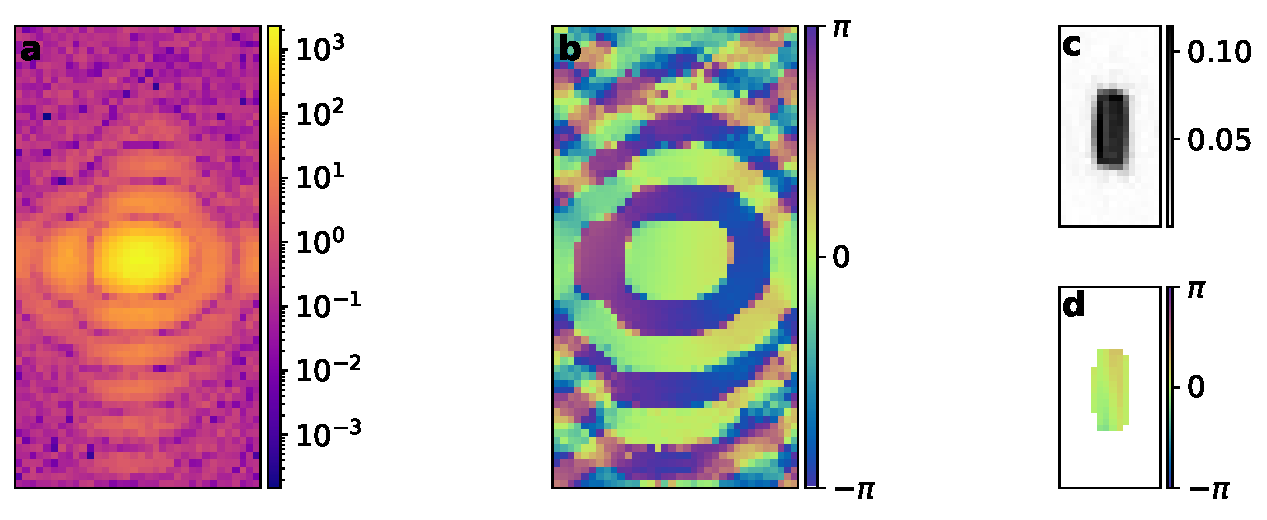
\includegraphics[width=.8\textwidth]{figures/Phasing/rec_space_phase.pdf}
    \caption{Central slice of a typical BCDI pattern (\textbf{a}) with the corresponding RSP (\textbf{b}) obtained after a 
    successful reconstruction of the object (modulus and phase in \textbf{c - d} respectively). It is clear the structural similarity between the diffracted intensity 
    in logarithmic scale and the RSP. Moreover, one can notice that in this case of low strain faceted particle, 
     the RSP varies regularly between 0 and $\pi$ (or $-\pi$) in correspondence of the intensity fringes. }
    \label{fig:rec_space_phase}
\end{figure}

Moreover, given this ``simple'' law of constructive-destructive interferences, we hypothesized the possibility to predict patches 
of this RSP given a portion of diffraction pattern and then, similarly to the inpainting case, stitch together them together
and obtain the full RSP. This entails a number of complications related to the so-called phase symmetries that I have encountered
during the development of the algorithms and that will be discussed in the next sections. \\
Ultimately, the goal of this DL model for phasing is to facilitate the reconstruction of highly strained particles. While 
other works in literature have mostly leveraged the gain in computing time, here the model aims at tackling those reconstructions for which 
conventional algorithms struggle to find convergence because of the high strain in the particle.   
However, in this case, the aforementioned RSP $\pi$-shifts in between two fringes is much more complicated since the 
strong and extended displacement fields inside the crystal alter the Bragg peak, merging and spreading the fringes 
into an irregularly distributed intensity pattern. I anticipate that this is what actually prevents the DL model 
from functioning on patches, for the high-strain case. It is however reported in this manuscript as it can help with the 
understanding of this complex problem and maybe serve in the future for further studies. 
% al punto che non si e' in grado di stabilire, a occhio, se l'informazione necessaria per costruire la mappa I-phi e' racchiusa in una porzione 
\section{Dataset creation} 

I have trained our model in a supervised manner, meaning, in this case, that the training was always conducted on simulated data 
only, as the RSP is never experimentally detectable. 
For this reason, I have simulated the training dataset following the same procedure described in Sections 
\ref{sec:dataset_creation2D} and \ref{sec:dataset_creation3D} for the 2D and 3D cases, respectively. However, in this
case, the dataset size was reduced to $64\times64\times64$ pixels, and no gap was applied. Additionally, I have used the 
calculated RSP as the ground truth label for training instead of the masked diffraction pattern.\\

I will anticipate here that for the high strain case I created a dedicated training set simulating the strain by applying 
an artificial ``strong'' phase to the particles. In order to have a diverse population of strain distributions I have 
simulated each object's phase using different functions and parameters, namely: with the sum of two Gaussian functions,
with the sum of two cosine functions and using a random Gaussian distribution. In each case, amplitudes, variances, 
frequencies, and correlation lengths were randomly chosen to ensure a phase variation within the particle ranging between 
$2\pi$ and $5\pi$. By doing this, I could obtain strongly distorted BCDI patterns, similar to experimental high-strain ones. 
In particular, the two Gaussian functions phase can closely emulate the effect of the substrate induced strain inside Winterbottom 
particles. 

\section{2D case low strain}\label{chp:2d_nostrain}
% MODEL 2D CASE NO STRAIN: SHOW THE MODEL PREDICTING THE PHASE AND USE A LOSS ON THE FOURIER TRANSFORM 
Alike the inpainting case, I have first conducted some preliminary studies in 2D, on noise-less low strain data. Here I will 
briefly show the model's architecture, the loss function and the results. 
\subsection{Model structure}
The architecture that I used has a U-Net like structure with an encoder and a decoder. 
The encoder is composed of six convolutional blocks through which the input diffracted intensity is progressively 
reduced from the 64 pixel-side squares to a 1D flattened vector. Each convolutional block is composed of a convolutional 
layer, a LeakyReLU activation function and a MaxPooling layer that halves the feature's map dimensions. (illustrate the 
parameters later). \\
At the end of the encoder the so-called bottleneck composed of a convolutional layer followed by a LeakyReLU activation 
processes the feature map before passing it to the decoder which, by means of transposed convolutions, LeakyReLU activations 
and UpSampling layers, brings back the feature map to the input's size. Skip connections between encoder and decoder blocks 
are employed as well. The output tensor is the result of a last single-channeled convolutional layer with no activation function. 
In this way we let the model predict unbounded tensors to account for the phase symmetries (see Intro). 

\subsection{Input preprocessing} 

Similarly to the inpainting case, the BCDI patterns have been transformed into logarithmic scale and normalized between 
0 and 1. Batches of 32 images at the time were used. 

\subsection{Loss function}
The choice of the loss function was firstly based on what was used in literature. 
A sum of the MSE computed on the objects' amplitudes and one on the phases has thus been used (Eq. \ref{eq:loss}). The ground truth 
objects were indeed available from the simulated data while the predicted objects have been first calculated with a 2D  
inverse Fourier transform from the diffracted amplitude and the predicted RSP (Eq. \ref{eq:ft_2D}). 
\begin{equation}
    \hat{o}(\mathbf{r})
    \;=\;
    \mathcal{F}^{-1}\!\bigl\{\sqrt{I(\mathbf{q})}\,e^{\,i\,\varphi_{\mathrm{pred}}(\mathbf{q})}\bigr\}(\mathbf{r})
    \quad,
    \label{eq:ft_2D}
\end{equation}

\begin{equation}
    \mathcal{L}
    \;=\;
    \frac{1}{N}\sum_{\mathbf{r}}
    \Bigl(\bigl|\hat{o}(\mathbf{r})\bigr|
        \;-\;\bigl|o(\mathbf{r})\bigr|\Bigr)^{2}
    \;+\;
    \frac{1}{N}\sum_{\mathbf{r}}
    \Bigl(\phi(\mathbf{r})
        \;-\;\phi_{\mathrm{gt}}(\mathbf{r})\Bigr)^{2}
    \quad,
    \label{eq:loss}
\end{equation}

\subsection{Results}
The training of the model was conducted on 8500 simulated BCDI patterns over 30 epochs with a learning rate of 0.0003
and monitored both training and validation loss. Here, Fig.\ref{fig:loss_2mse_nosymm} shows the model's loss during the 
30 epoch long training. However, despite the good decaying trend, typical of proper training, the model does not 
perform optimally when tested on new data. 

\begin{figure}[H]
    \centering
    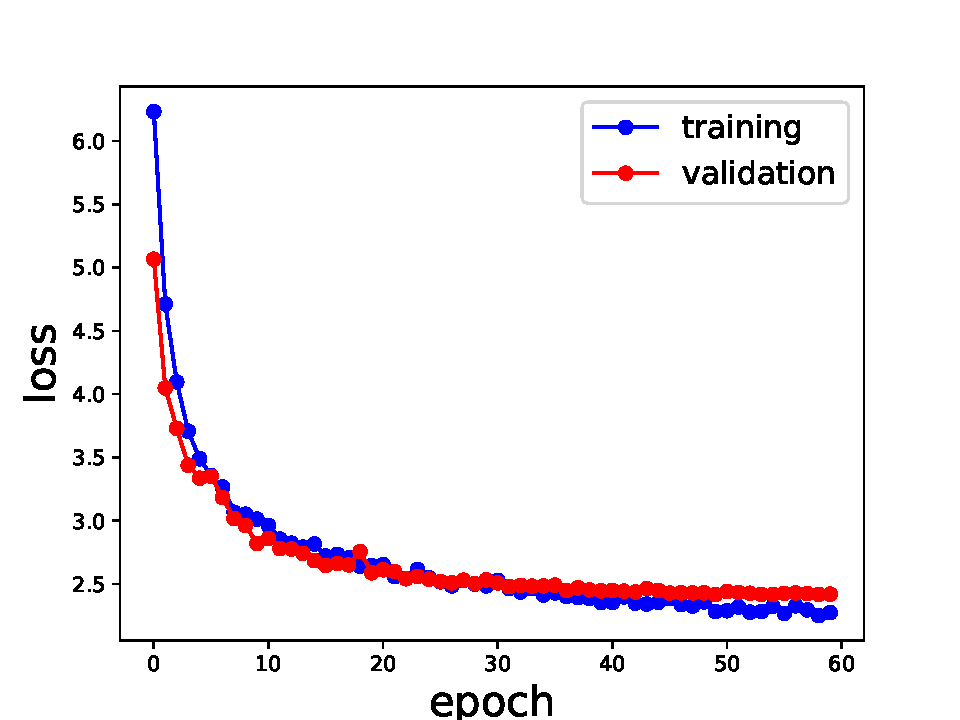
\includegraphics[width=.8\textwidth]{figures/Phasing/loss_low_strain_noiseless_doubleMSE_nosymm.pdf}
    \caption{Training and validation loss over 30 epochs. The curve suggests a proper learning with no overfitting as 
    both losses are decreasing reaching a plateau and the validation loss follows the same trend of the training loss.}
    \label{fig:loss_2mse_nosymm}
\end{figure}

Fig.\ref{fig:RSP_lowStrain_doubleMSE} illustrates the results of the predicted RSP of some test simulated BCDI patterns. 
Note that the displayed predicted RSP has been wrapped between 0 and 2$\pi$ for better comparison with the ground truth 
but the raw output of the model is in fact an ``unwrapped'' array. This is expected since no activation layer was applied 
to the last convolutional layer, meaning that the last operation is the multiplication of the last feature map with the 
real values inside the convolutional kernel, hence linear. \\
When comparing the reconstructed objects obtained from the predicted RSP with the ground truth ones (Fig. \ref{fig:obj_lowStrain_doubleMSE})
one can draw some interesting conclusions about the model's learning performances. 
First it can be observed that the model learns the approximate shape and size of the particle, it produces indeed images 
that resemble reasonable particles, sometimes similar to the ground truth ones. The amplitude is concentrated inside 
the support with little noise outside and the phase is overall correct around zero. However, when looking more carefully, 
it is clear that the shape is not quite correct, especially for highly non-centrosymmetric objects. For instance, if we 
consider the object in Fig. \ref{fig:obj_lowStrain_doubleMSE} \textbf{c}, we see that the predicted shape seems to be 
deriving from the incorrect superposition of the correct shape and its twin, as well correct. More in general it seems 
that the model tends to predict centrosymmetric objects. According to Sicairos \textit{et al.} \cite{guizar-sicairos_understanding_2012}, 
if we name $\varphi(\vec{q})$ the correct RSP, this phenomenon is originated by a predicted RSP phase $\phi$ composed 
of $\varphi(\vec{q})$ in some regions of the $q$-space and $-\varphi(\vec{q})$ elsewhere. In other words, the model is not 
fully able to break the sign symmetry. This subject was recently studied by Zhang and coauthors in \cite{zhang_what_2024}. 
In their study, the authors show that if not broken in the dataset, meaning that during the 
training the model is exposed to both cases ($\varphi(\vec{q})$ and $-\varphi(\vec{q})$) indistinctly, the model is deceived 
to a mix of the two, since the sign information cannot be recovered from the input intensity. The authors conclude that 
in order prevent this detrimental effect, one should break the symmetry in the dataset to bias the model towards one 
preferred sign. 

\begin{figure}[H]
    \centering
    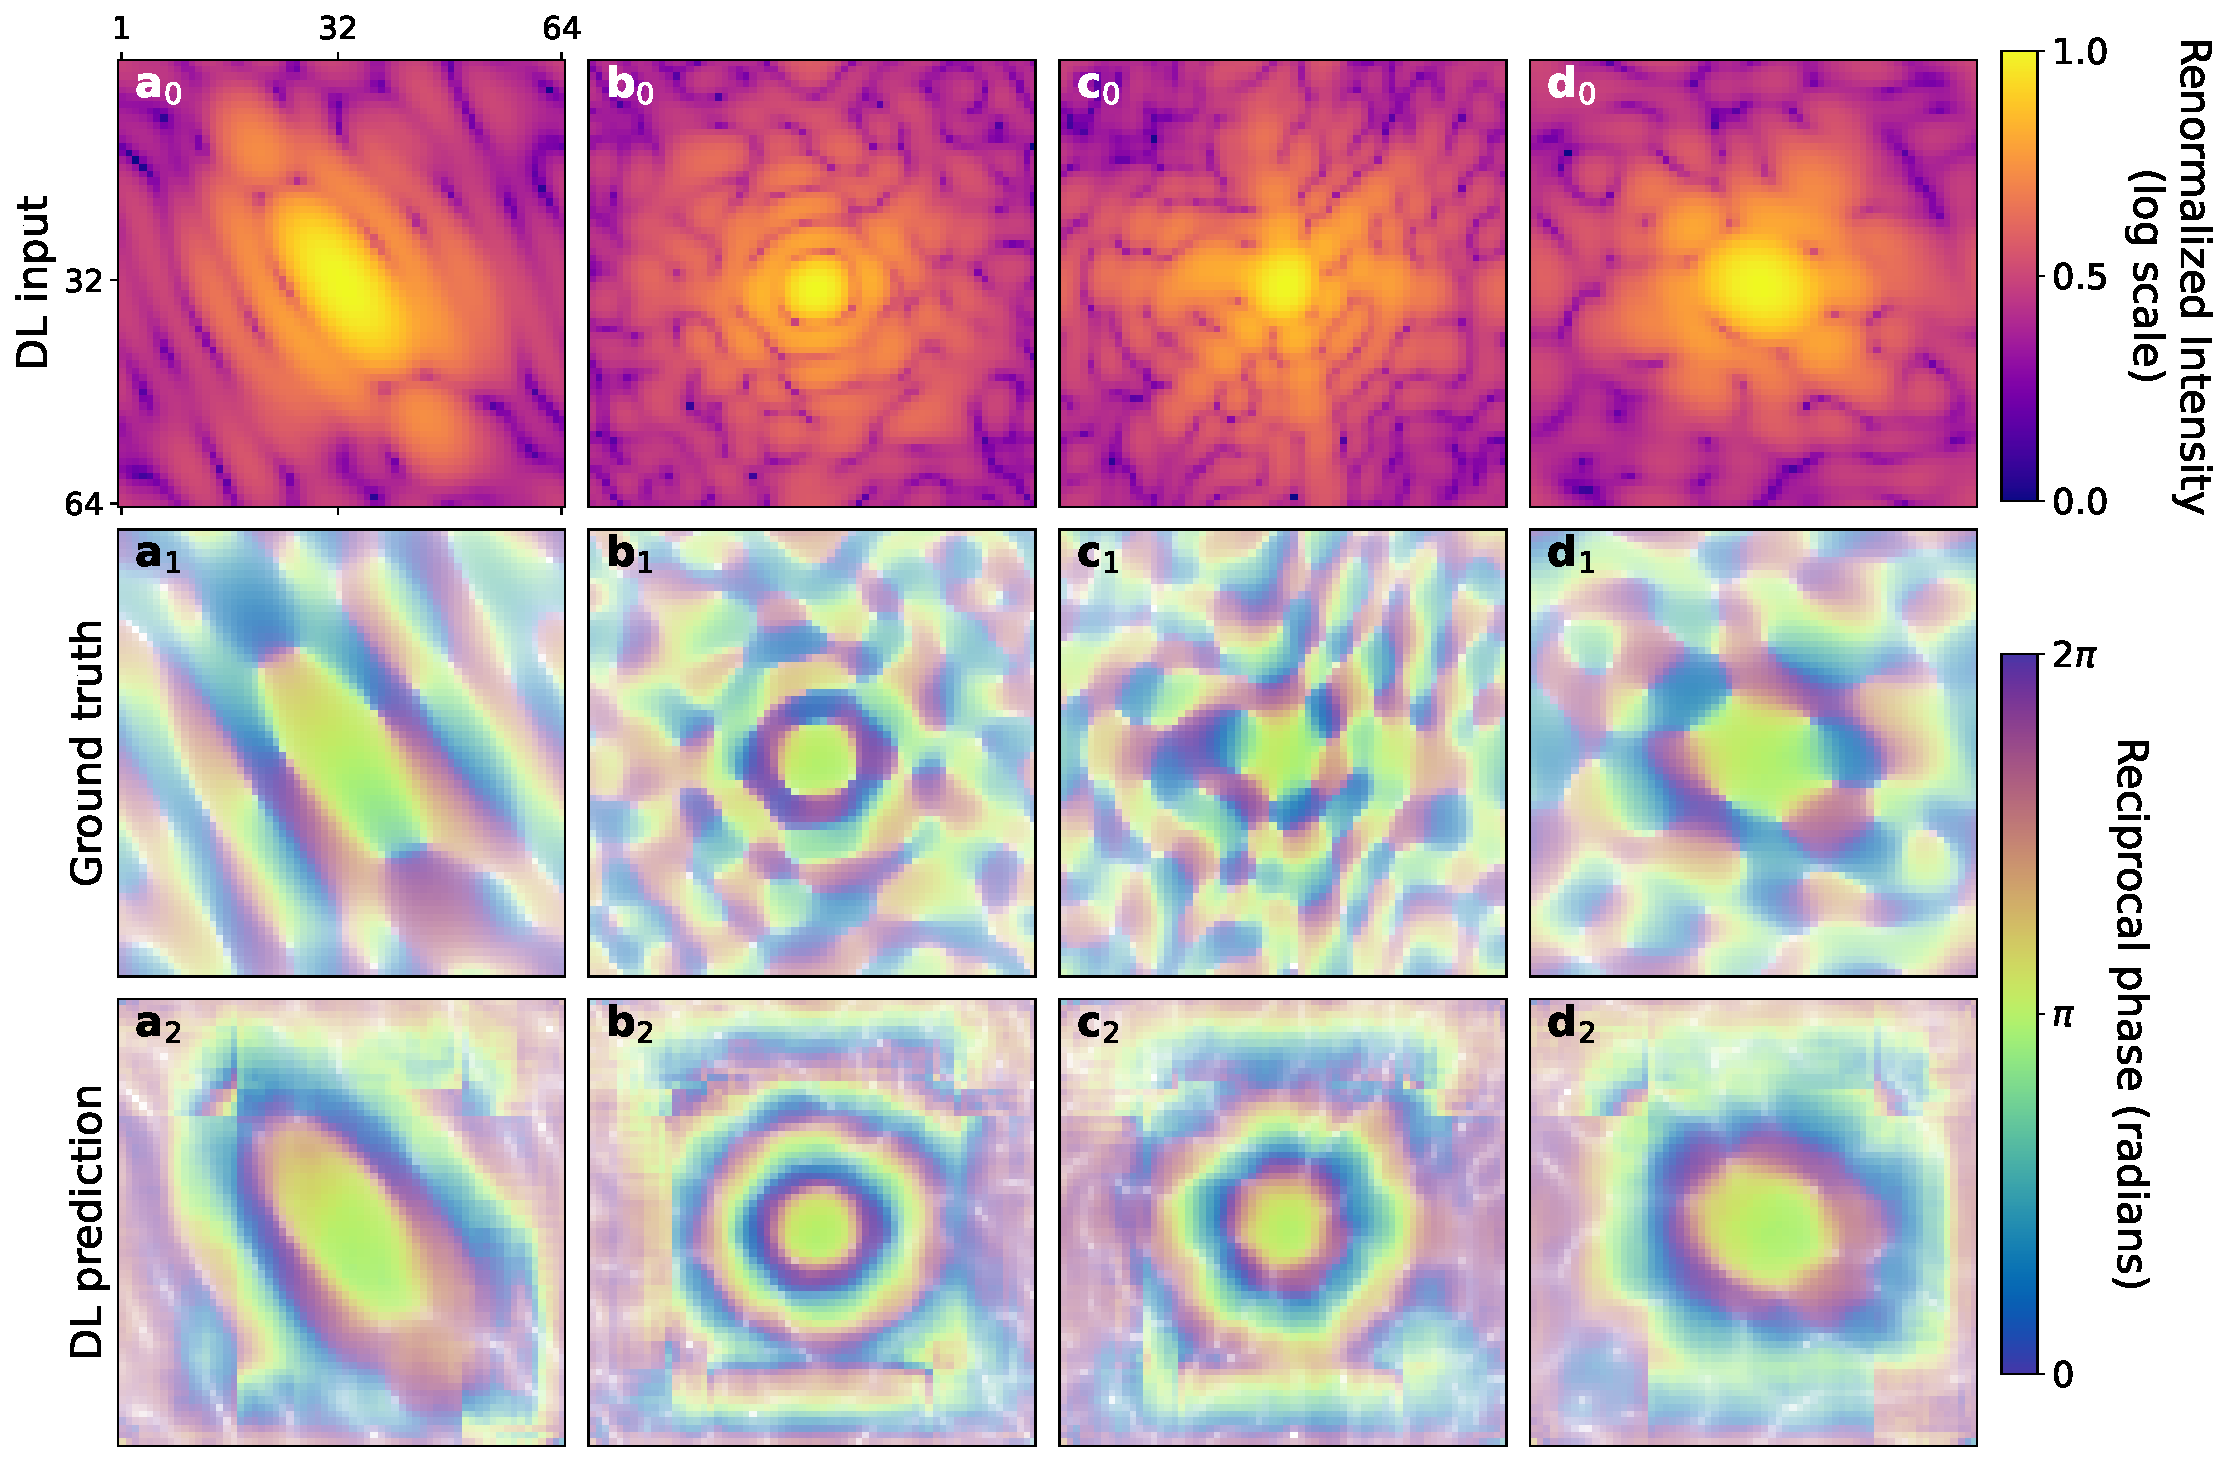
\includegraphics[width=.8\textwidth]{figures/Phasing/RSP_low_strain_doubleMSE.pdf}
    \caption{\textbf{Model testing on new 2D data using MSE loss function}. First row shows four simulated BCDI patterns, second row the ground truth RSP 
    corresponding to the pattern and last row the DL prediction }
    \label{fig:RSP_lowStrain_doubleMSE}
\end{figure}
\begin{figure}[H]
    \centering
    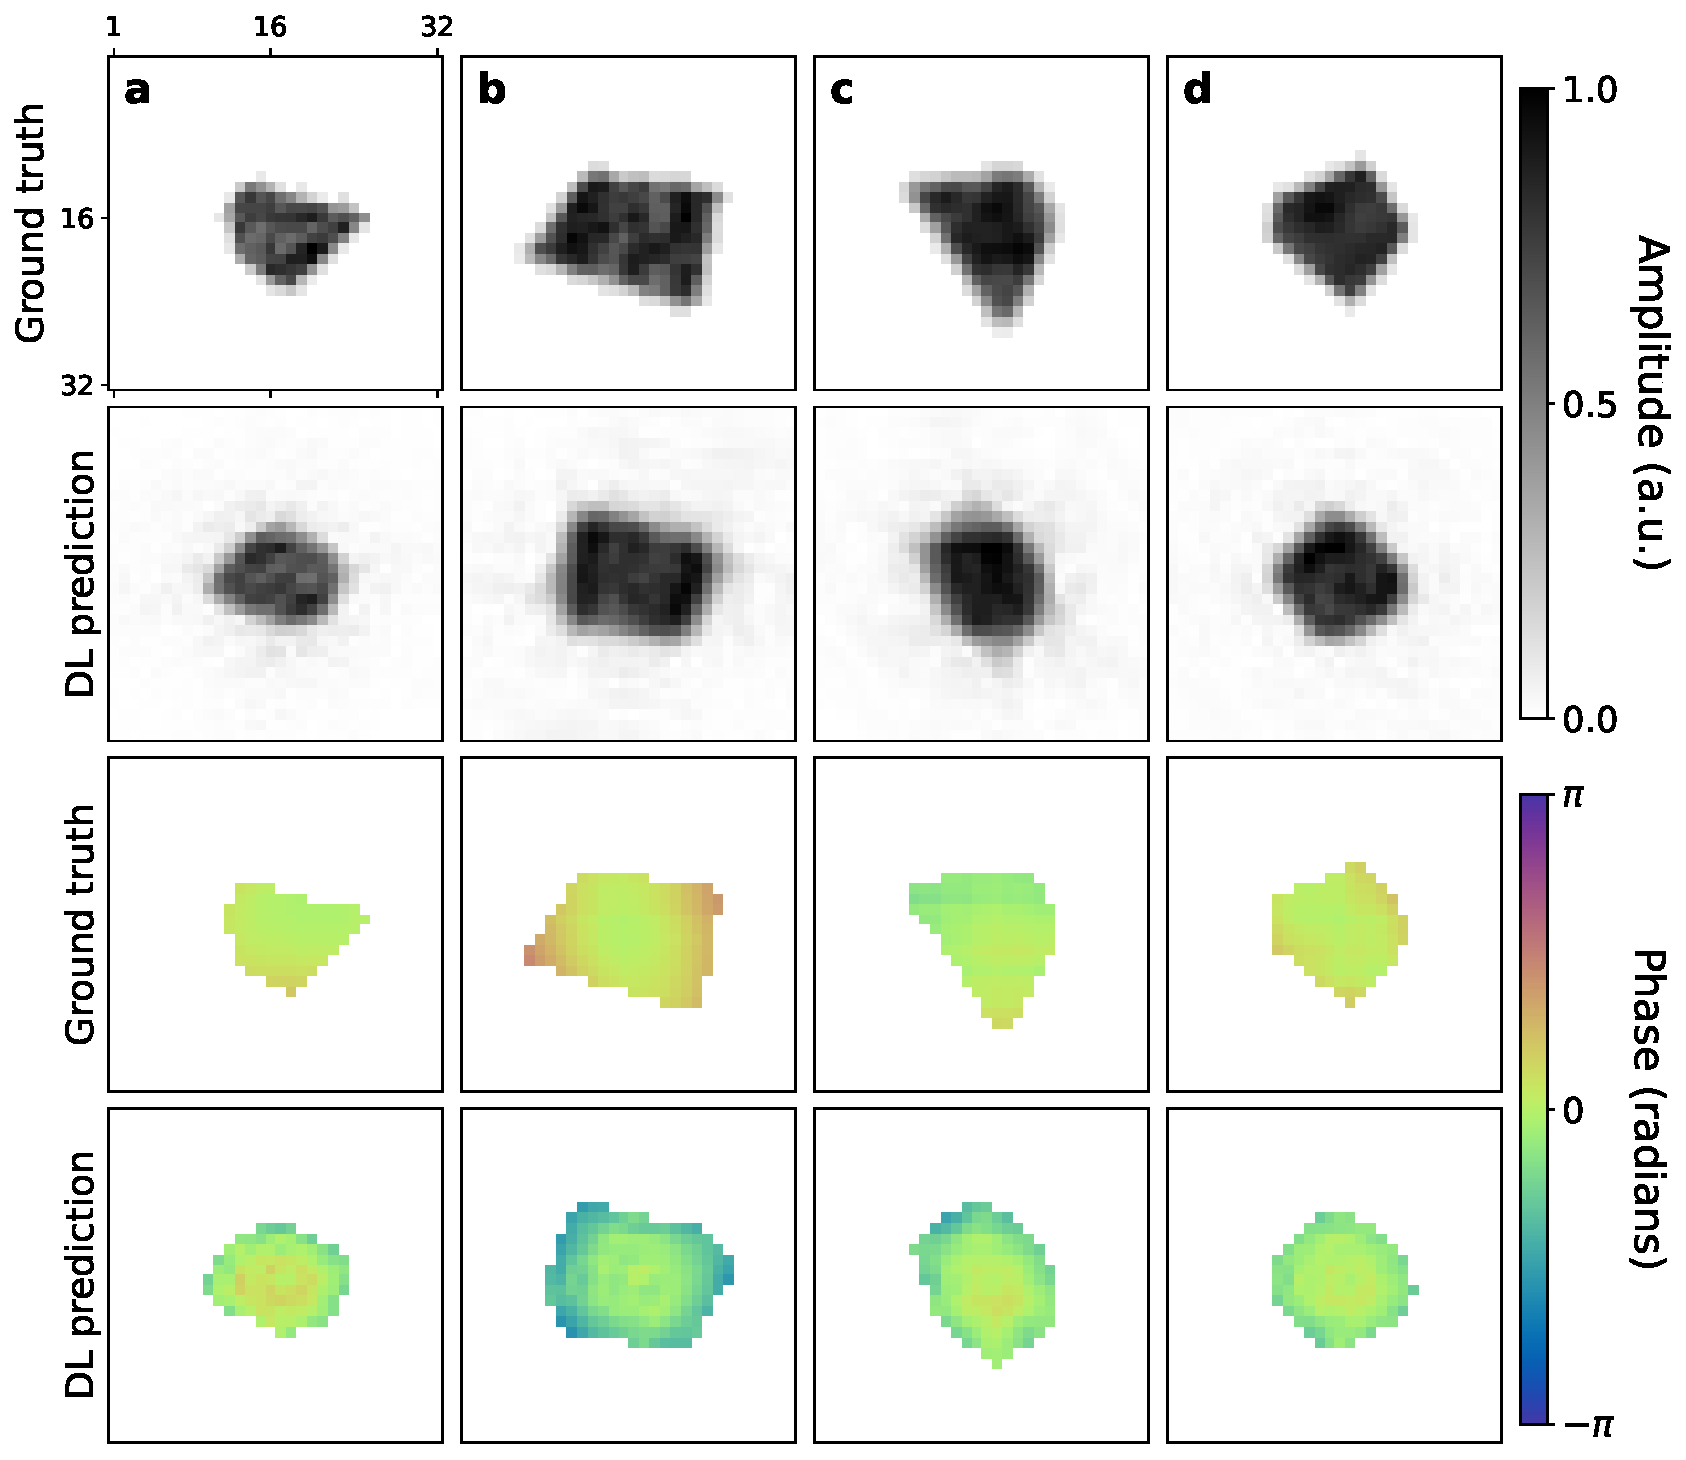
\includegraphics[width=.8\textwidth]{figures/Phasing/obj_low_strain_doubleMSE.pdf}
    \caption{\textbf{Corresponding reconstructed objects}. Ground truth and predicted objects' amplitudes (first two rows 
    respectively) and ground truth and predicted objects' phases (first two rows respectively)}
    \label{fig:obj_lowStrain_doubleMSE}
\end{figure}


The procedure presented in the article for the removal of the phase symmetries consists in: (i) the centering of all the 
objects in real space (phase ramp removal), (ii) the shift of the RSP such that the zero value in the same array position 
across the dataset (phase offset removal), and lastly, (iii) they flip the sign of the RSP when its value in corresponding 
to a fixed position across the dataset is negative. In our case the phase ramp symmetry was already broken by simulating 
particles with the center of mass in the center of the array. In this way the model is already biased towards the prediction 
of RSPs that yield centered objects. For the offset and the sign, the method proposed by Zhang \textit{et al.} has been 
implemented in the model and the results are shown in Fig. \ref{fig:RSP_lowStrain_doubleMSE_JuSun} for the RSP and 
Fig. \ref{fig:obj_lowStrain_doubleMSE_JuSun} for the reconstructed objects. 

\begin{figure}[H]
    \centering
    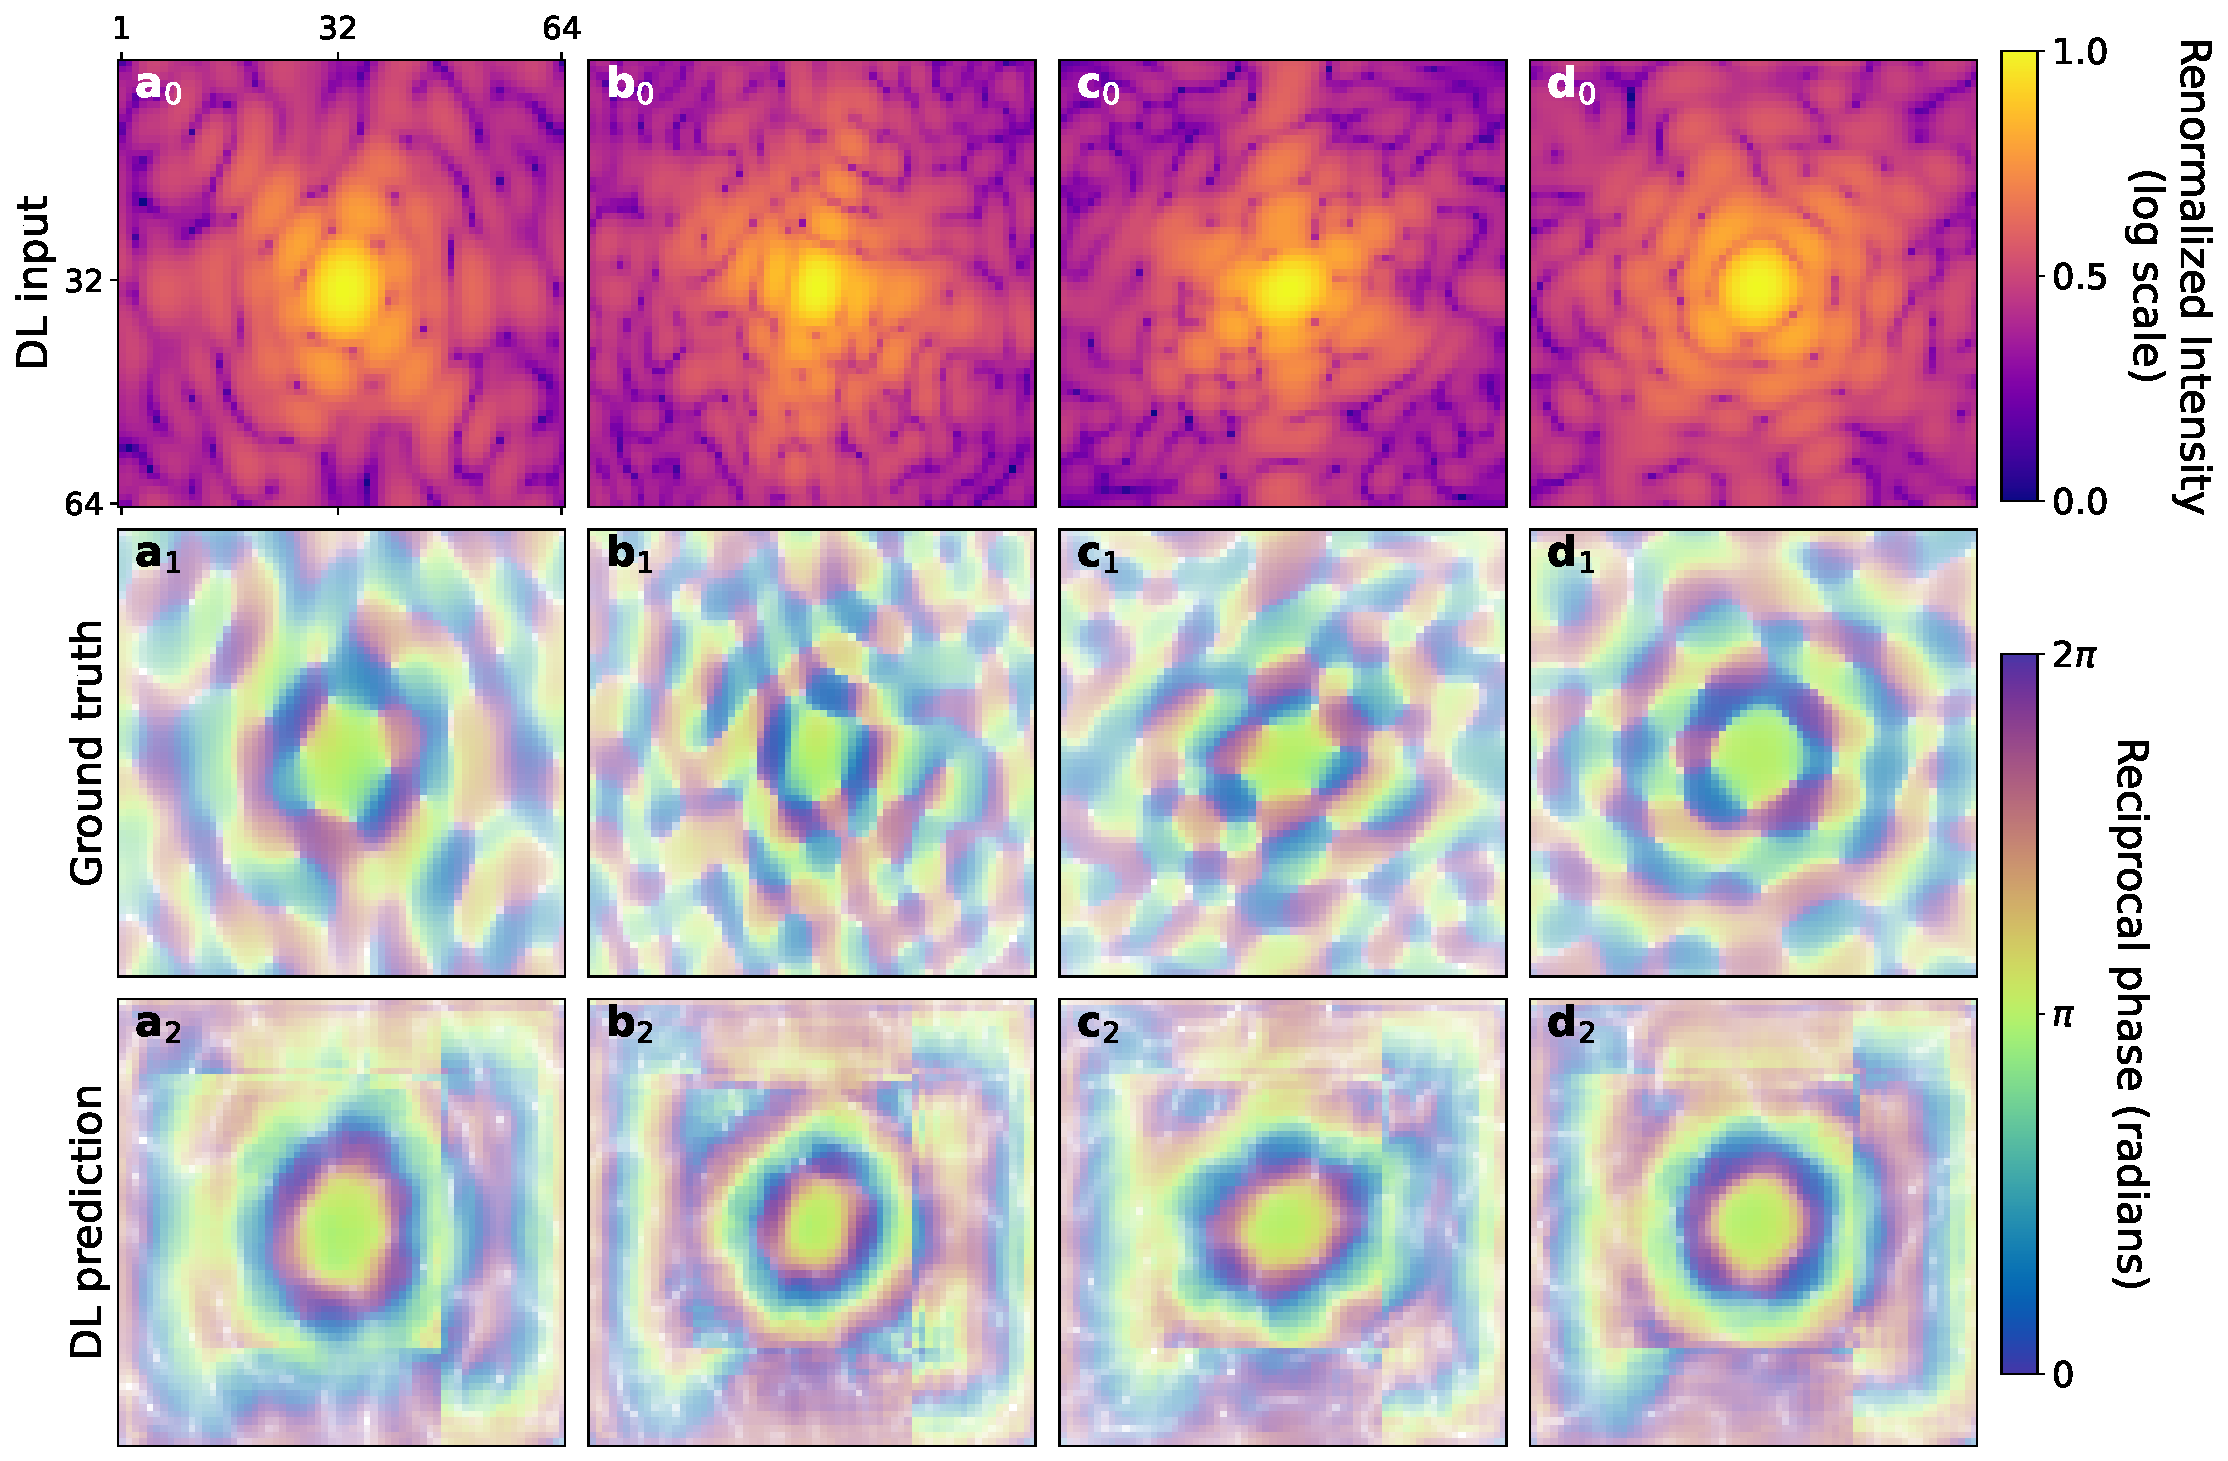
\includegraphics[width=.8\textwidth]{figures/Phasing/RSP_low_strain_doubleMSE_symmJuSun.pdf}
    \caption{\textbf{Model testing using MSE loss function and biased dataset}. First row shows four simulated BCDI patterns, second row the ground truth RSP 
    corresponding to the pattern and last row the DL prediction }
    \label{fig:RSP_lowStrain_doubleMSE_JuSun}
\end{figure}

\begin{figure}[H]
    \centering
    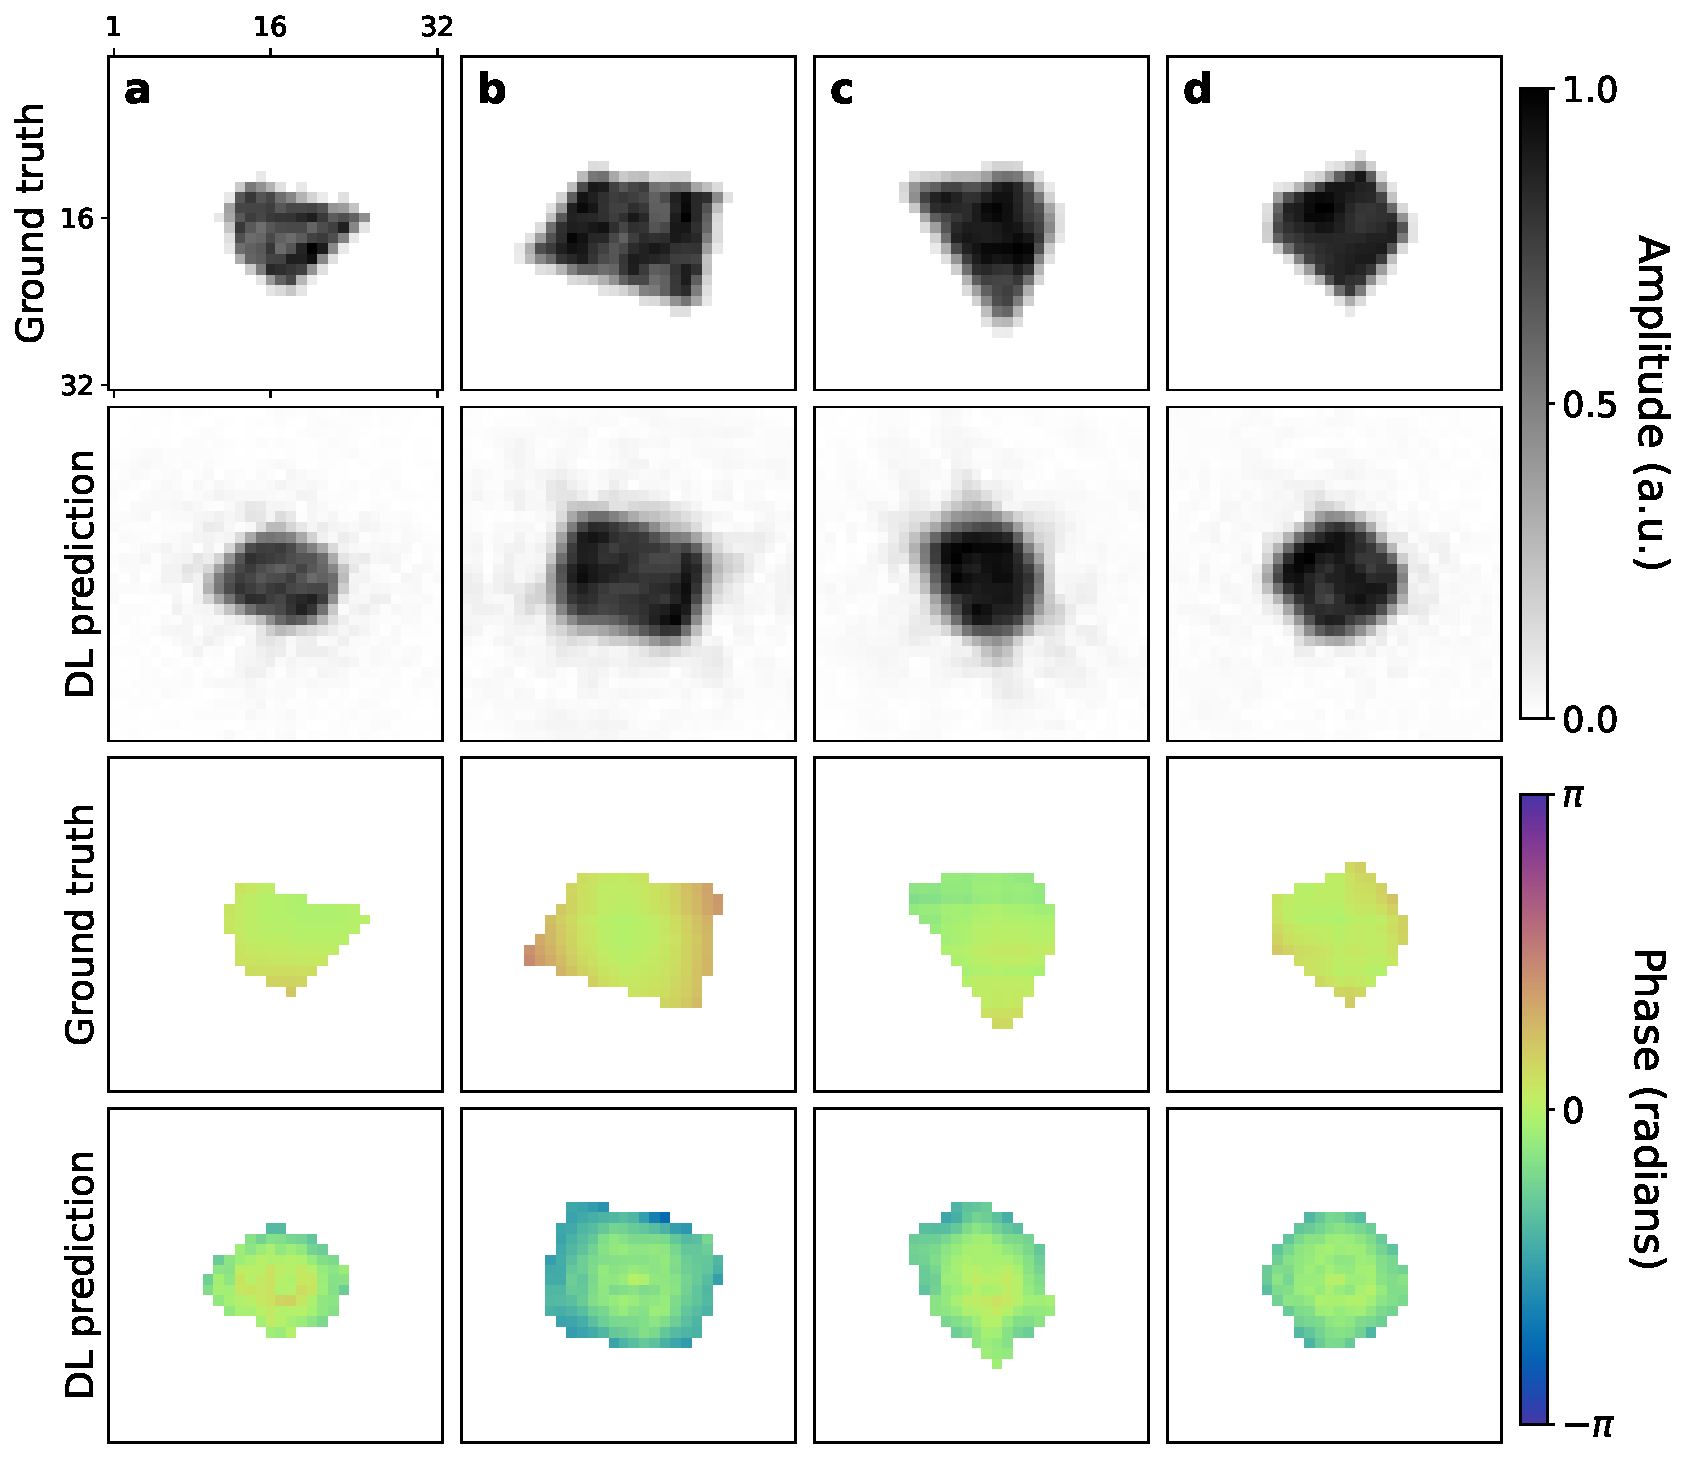
\includegraphics[width=.8\textwidth]{figures/Phasing/obj_low_strain_doubleMSE_symmJuSun.pdf}
    \caption{\textbf{Corresponding reconstructed objects}. Ground truth and predicted objects' amplitudes (first two rows 
    respectively) and ground truth and predicted objects' phases (first two rows respectively). No significant improvement 
    can be observed after the adopted sing-symmetry breaking procedure.}
    \label{fig:obj_lowStrain_doubleMSE_JuSun}
\end{figure}

Unfortunately, the proposed method did not seem to solve the sign ambiguity of the RSP. The model is still unable to 
discriminate between the plus/minus sign of the RSP and the result is the incorrect overlap of the object with its twin
obtained by the inversion symmetry. The phase, though small for this case, is also showing a kind of centro-symmetry 
as its variations tend to spread radially from the center of the array. 

\subsection{The Weighted Coherent Average loss function}
At this point in the study, and in anticipation of applying the model to portions of the RSP, it became necessary to 
consider a loss function that would operate directly on the phase, without requiring transformations into real space. 
However, the main challenges were posed by the symmetries inherent to the phase. Upon further reflection, it was concluded
that a Mean Squared Error (MSE) is not an appropriate metric for comparing the phases of complex functions. Indeed, MSE 
fails to account for the 2$\pi$ periodicity and the possibility of a global phase offset. One could argue that 2$\pi$ wraps 
can be fixed with a modulo 2$\pi$ operation and the offset can be removed by shifting the tensor by a constant. However, 
the modulo wrapping function jumps abruptly by 2$\pi$ every time phase crosses an integer multiple of 2$\pi$, meaning that 
the gradients are infinite thus not advised for gradient-based optimizations. Moreover, the MSE (or MAE and other 
\textit{divergent} metrics) will have problems at the 0-2$\pi$ boundary. In fact, when considering the phase mapped in the
0-2$\pi$ range, if we suppose a $\varphi_{pred}^0 = -0.1$ where $\varphi_{G.T.}^0 = 0$, the wrap will move the $\varphi_{pred}^0$ to the value 
$2\pi - 0.1 = 6.183$ amplifying the error ( $\Delta )$ from $0.1^2$ to $6.183^2$ improperly.
\\
In order to bypass these shortcomings a new loss function was designed. Here it follows the reasoning process that leads
to the mathematical expression of the loss. \\
The best way to account for the periodicity and the wrap without discontinuities 
and error unbalances, is to evaluate the ground truth - predicted phase differences ($\Delta_k$) on the unit circle. 
To do such, it's necessary to express $\Delta_k$ as angles of a complex exponential. This means that if $\varphi_{pred}$ is an array of 
random values, each complex number $ z_k = e^{(i\Delta_k)}$, when represented on the Argand plane, can be seen as a 
vector pointing at a random coordinate on the unit circle. Now, the goal of the optimization is not to minimize $\Delta_k$ 
for all $k$ but to have the same $\Delta_k$ throughout $k$. In fact, for $\varphi_{pred} \Leftrightarrow \varphi_{G.T.}$ each 
vector $z_k$ points in the same direction, but it does not necessarily lie on the x-axis ($\Delta_k = 0 $ condition). 
Therefore, the loss function should ultimately drive all the $z_k$ from randomly distributed to coherently aligned along a common 
direction. A helpful quantity in this case can be the complex average vector $\langle z \rangle = \sum_{k=1}^{N}z_k = \sum_{k=1}^{N}e^{(i\Delta_k)}$
where $k$ runs over all the $N$ pixels. In particular the length of $\langle z \rangle$ , represented by the modulus $|\langle z \rangle|$,
is an efficient metric for the measurement of the degree of ``coherence'' among all the complex phase differences. 
In fact, $|\langle z \rangle|$ scores 0 for randomly oriented $z_k$, as opposite contributions cancel out each other because 
incoherent, while it scores 1 for perfectly aligned ones. It follows that one wants to maximize $|\langle z \rangle|$ during the 
optimization. Moreover, given the natural normalization between 0 and 1 of this metric, it follows naturally that the loss 
function can be expressed as $ L =  1 - |\langle z \rangle| $. \\
Additionally, an importance mask can be applied during the averaging process. In particular, we know that the brightest 
pixels of the BCDI pattern are the ones contributing the most to the object's reconstruction. For this reason one could 
weigh the complex average multiplying by the input magnitudes. The effect of this operation is to ``give a direction'' to the 
optimization, meaning that the $\langle \Delta \rangle $ the model will tend to converge to, will be mostly steered close to 
the $\Delta_k$ of the brightest $k$ pixels. 
The loss can now be expressed as: 

\begin{equation}
    L = 1 - \left|\frac{1}{N}\sum_{k=1}^{N} \sqrt{I_{k}}\exp\left(i(\varphi_{\text{GT},k} - \varphi_{\text{pred},k})\right)\right|
\label{eq:WCA_1}
\end{equation}

Where $N$ is the total number of pixels in each RSP array and $k$ is the pixel index. $\sqrt{I}$ is the magnitude of the BCDI pattern 
normalized between 0 and 1 with respect to the sum, and $\varphi_{\text{GT}}$ and $ \varphi_{\text{pred}}$ the ground truth and 
predicted RSP. \\
The last missing piece is the removal of sign symmetry. Rather than biasing the dataset preferring one sign over the opposite, 
the function $L$ is computed for both $\varphi_{\text{GT}}$ and $-\varphi_{\text{GT}}$ and in a second passage, the minimum of the two 
along the batch dimension is kept for backpropagation. The final form of the Weighted Coherent Average (WCA) loss is then given 
by: 

\begin{equation}
    L_{\text{WCA}} = \min\left(L_+, L_-\right)
\label{eq:WCA_2}
\end{equation}

To better visualize the functioning of the WCA loss function, a simple model has been trained to fit the ground truth phase 
of a single 2D BCDI pattern using the WCA. The complex phase differences vectors were extracted at each step of the optimization 
together with the updates obtained from the gradients of the WCA with respect to the trainable parameters. Fig. \ref{fig:WCA} 
shows the evolution of the predicted RSP as well as the progressive alignment of the  $z_k$.
\begin{figure}[H]
    \centering
    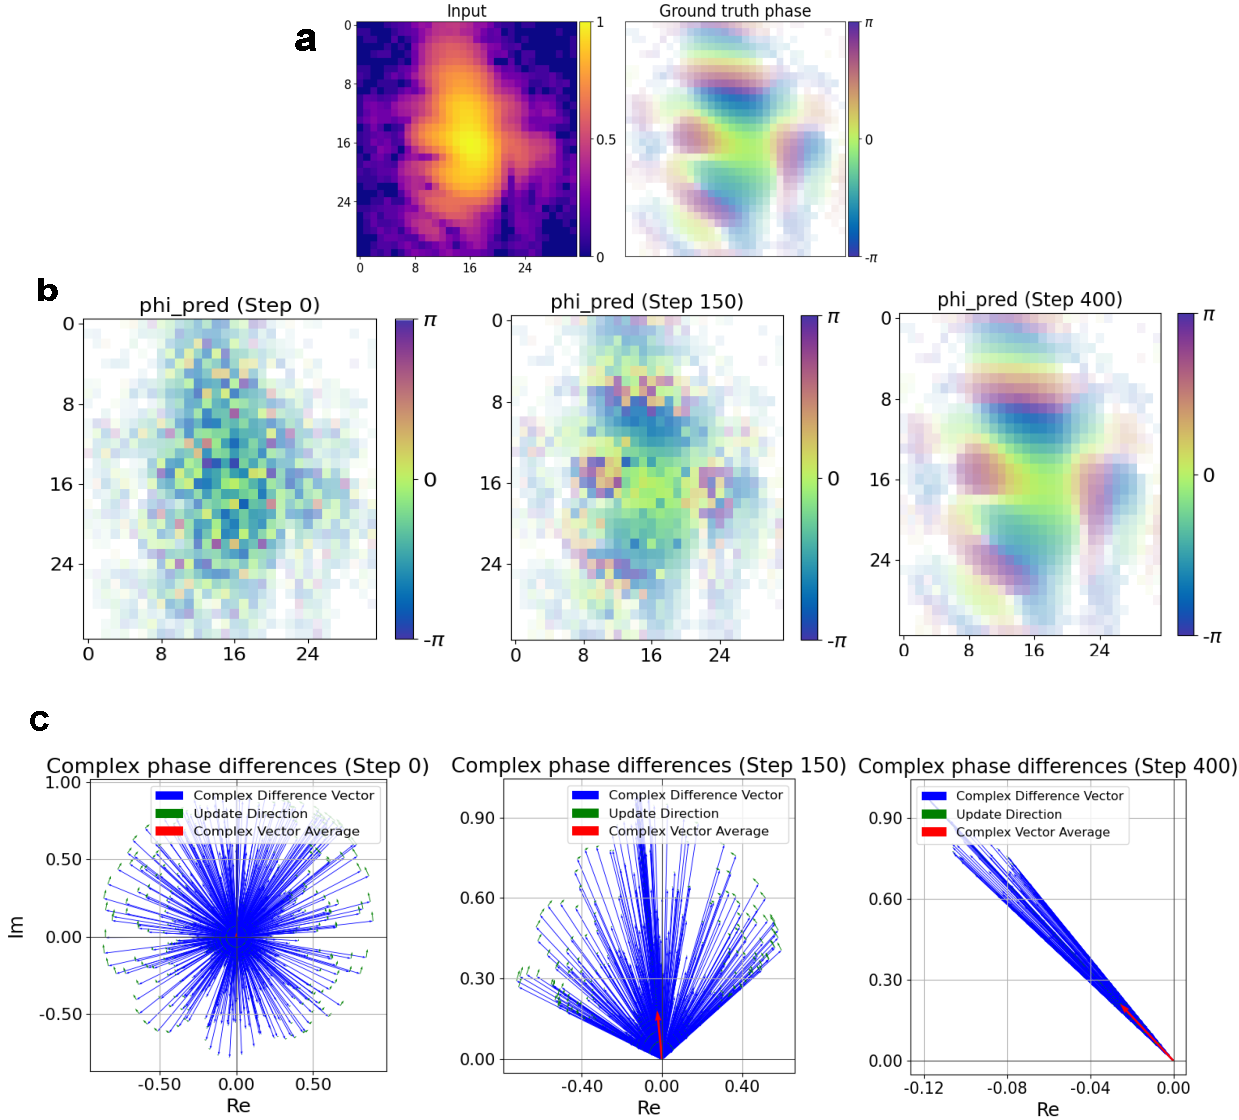
\includegraphics[width=.8\textwidth]{figures/Phasing/WCA.pdf}
    \caption{\textbf{Illustration of the WCA loss function}. \textbf{a} Input intensity (log-scale normalized) and
    ground truth RSP. \textbf{b} Predicted RSP in steps 0 - 150 - 400 of the optimization. \textbf{c} Corresponding 
    complex phase-differences vectors $z_k$ on the Argand plane (blue arrows), together with the updates (green arrows) obtained 
    from the gradients of the WCA, and the resultant complex average $\langle z \rangle$ (red arrow). It is visible that 
    during the fit, as the $z_k$ align around a common one, the amplitude of $\langle z \rangle$ grows bigger and the predicted 
    RSP converges to the ground truth one.}
    \label{fig:WCA}
\end{figure}

The same model has been trained using the WCA for the same number of epochs on the same dataset and here the results are 
shown. First, it can be noticed in Fig.\ref{fig:loss_vfn} that the training and validation loss values throughout the 
training are following different trends with respect to the model trained with the MSE loss (Fig. \ref{fig:loss_2mse_nosymm})

\begin{figure}[H]
    \centering
    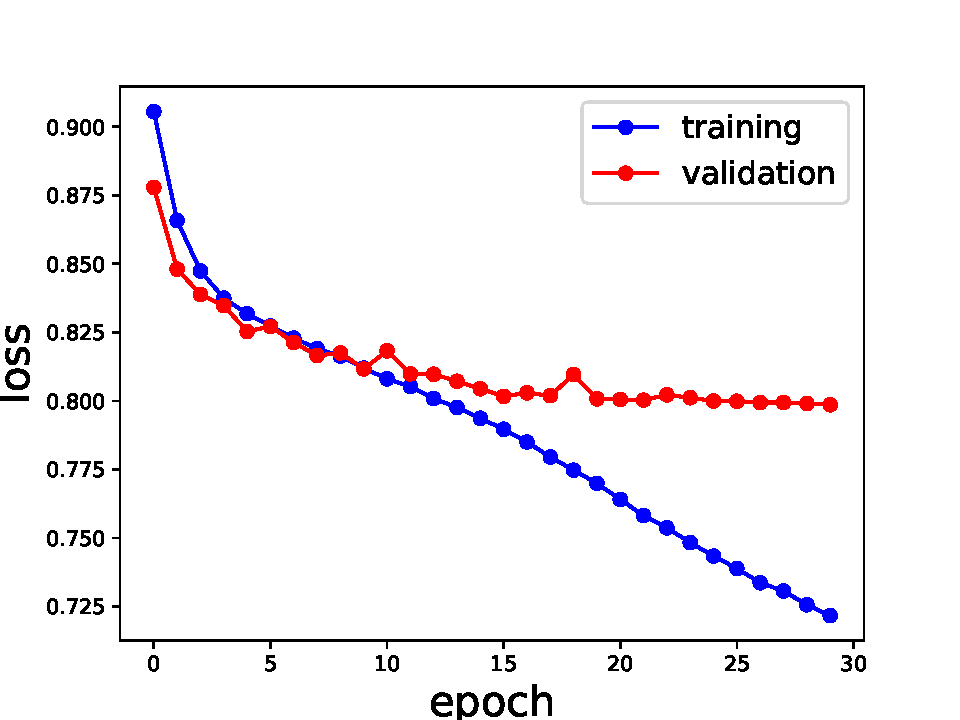
\includegraphics[width=.8\textwidth]{figures/Phasing/loss_low_strain_noiseless_doubleVFN.pdf}
    \caption{Training and validation loss curves over 60 epochs.}
    \label{fig:loss_vfn}
\end{figure}

In this case the correct learning curve does not reach a plateau within the first 25 epochs but maintains a negative slope 
for longer, indicating a better learning. This suggests indeed better results when used on test data. 
In particular, for the same input diffraction patterns tested above in Figs.\ref{fig:RSP_lowStrain_doubleMSE_JuSun} - \ref{fig:obj_lowStrain_doubleMSE_JuSun}
the model trained with the WCA yields the prediction shown in Fig.\ref{fig:RSP_vfn} for the RSP and Fig.\ref{fig:obj_vfn} 
for the corresponding reconstructed objects. 

\begin{figure}[H]
    \centering
    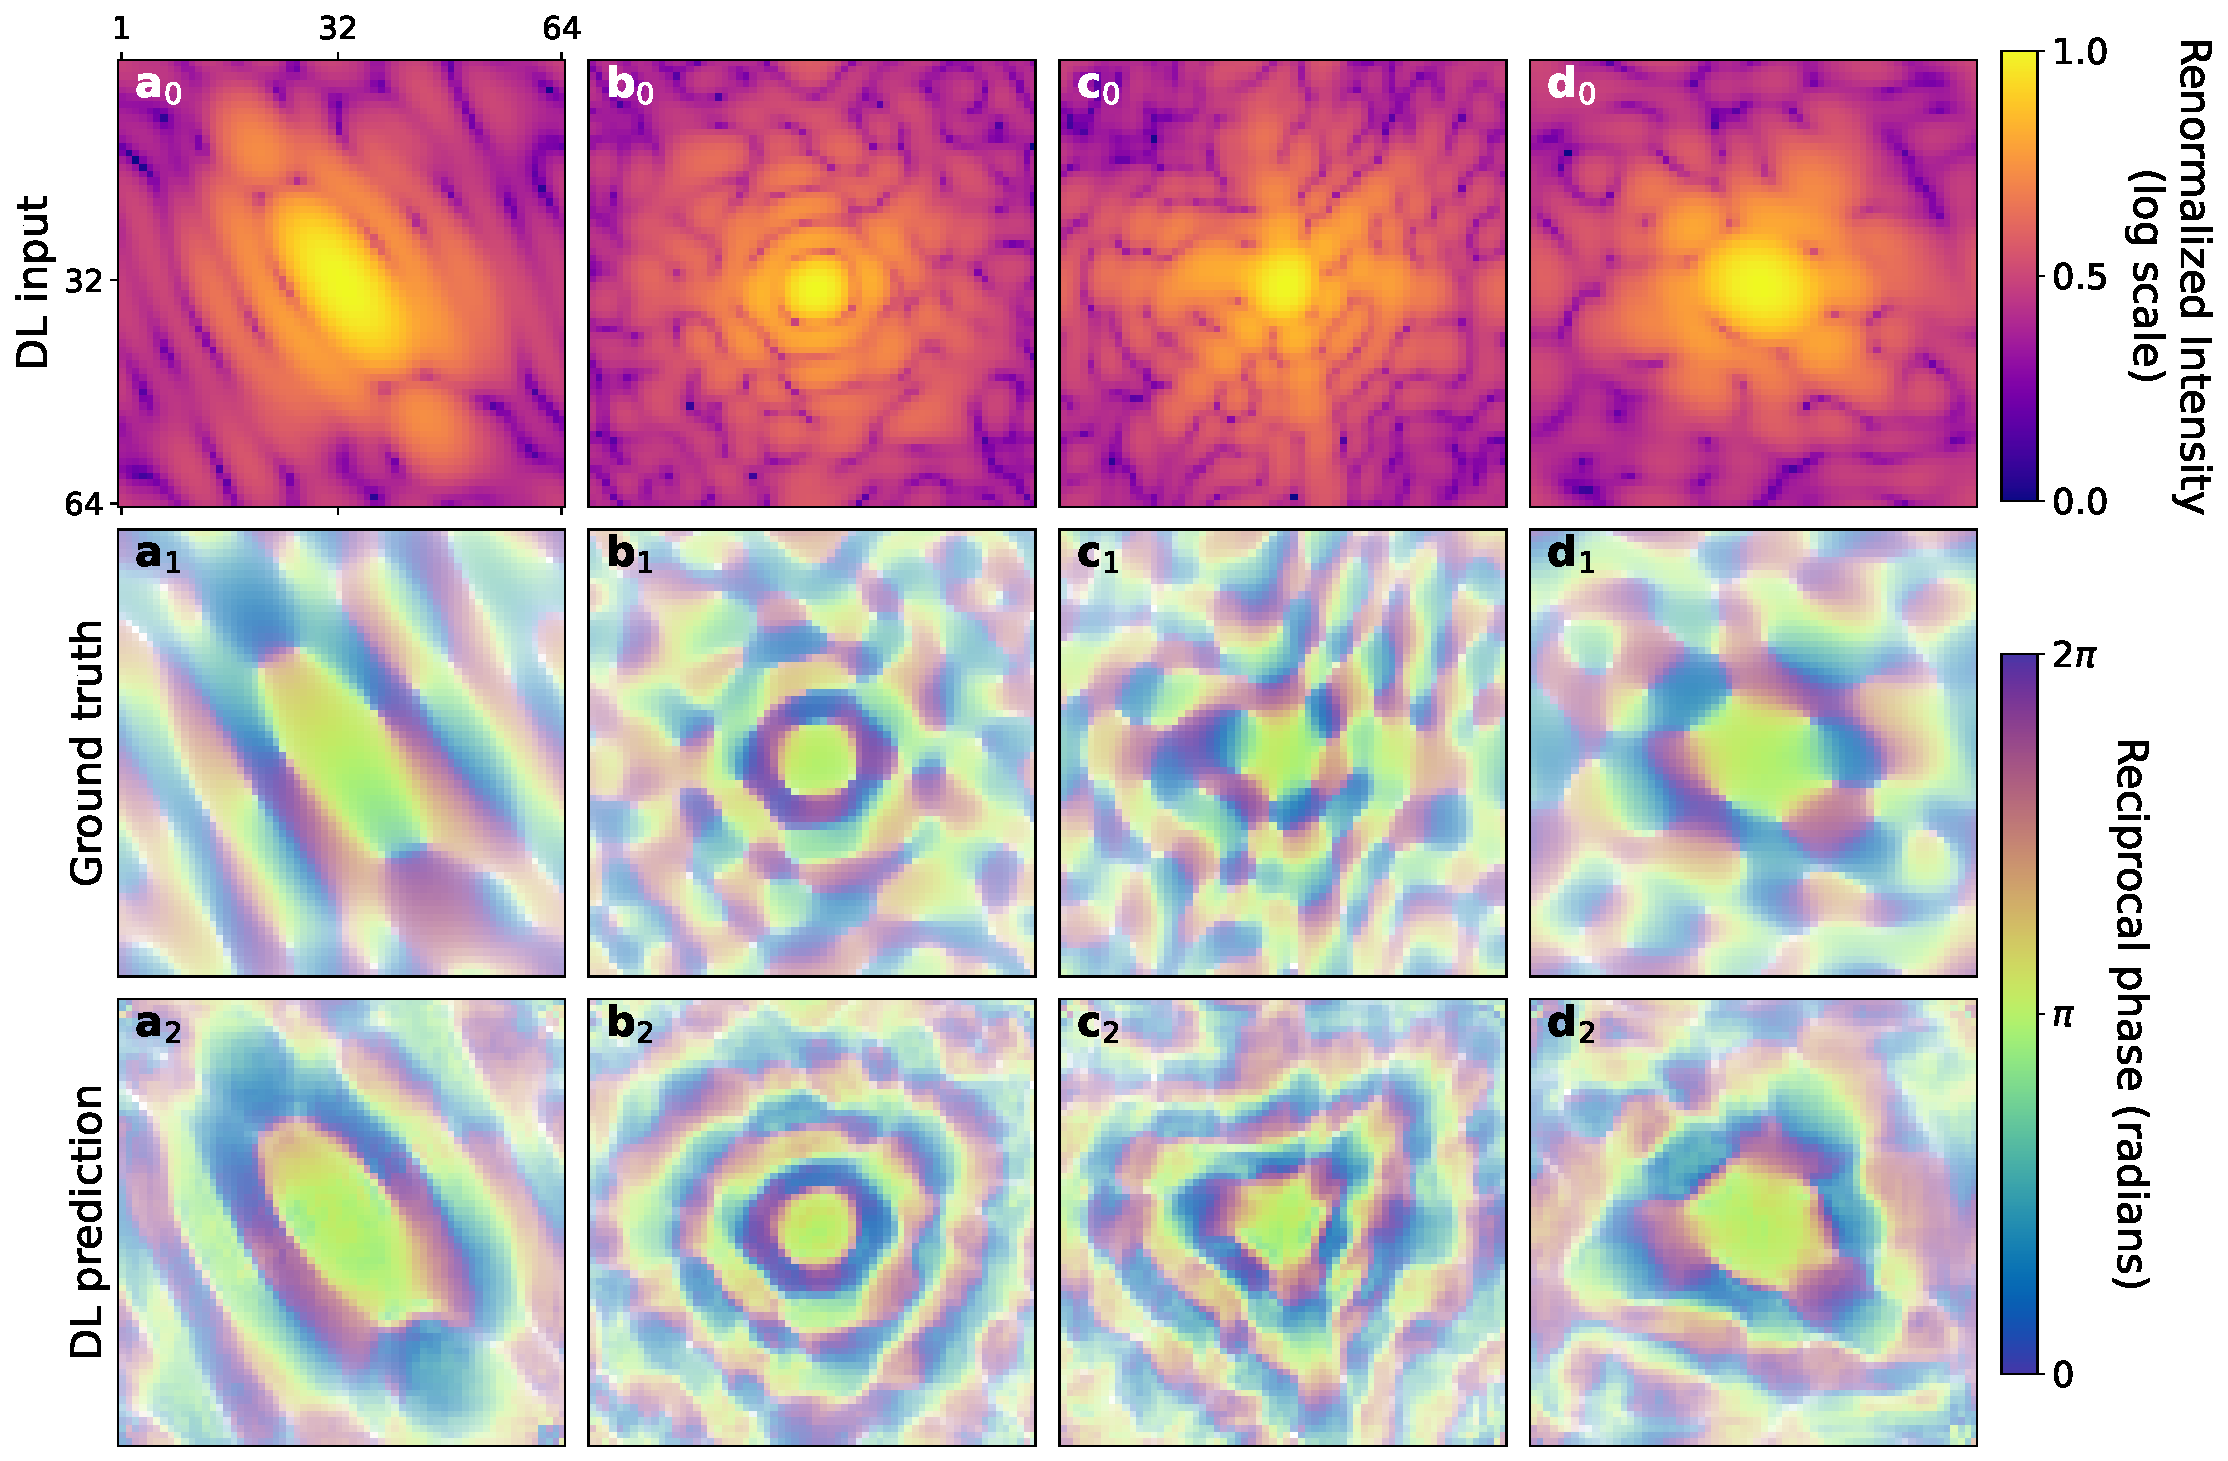
\includegraphics[width=.8\textwidth]{figures/Phasing/RSP_low_strain_VFN.pdf}
    \caption{\textbf{Model testing using WCA loss function}. First row shows four simulated BCDI patterns, second row the ground truth RSP 
    corresponding to the pattern and last row the DL prediction }
    \label{fig:RSP_vfn}
\end{figure}
\begin{figure}[H]
    \centering
    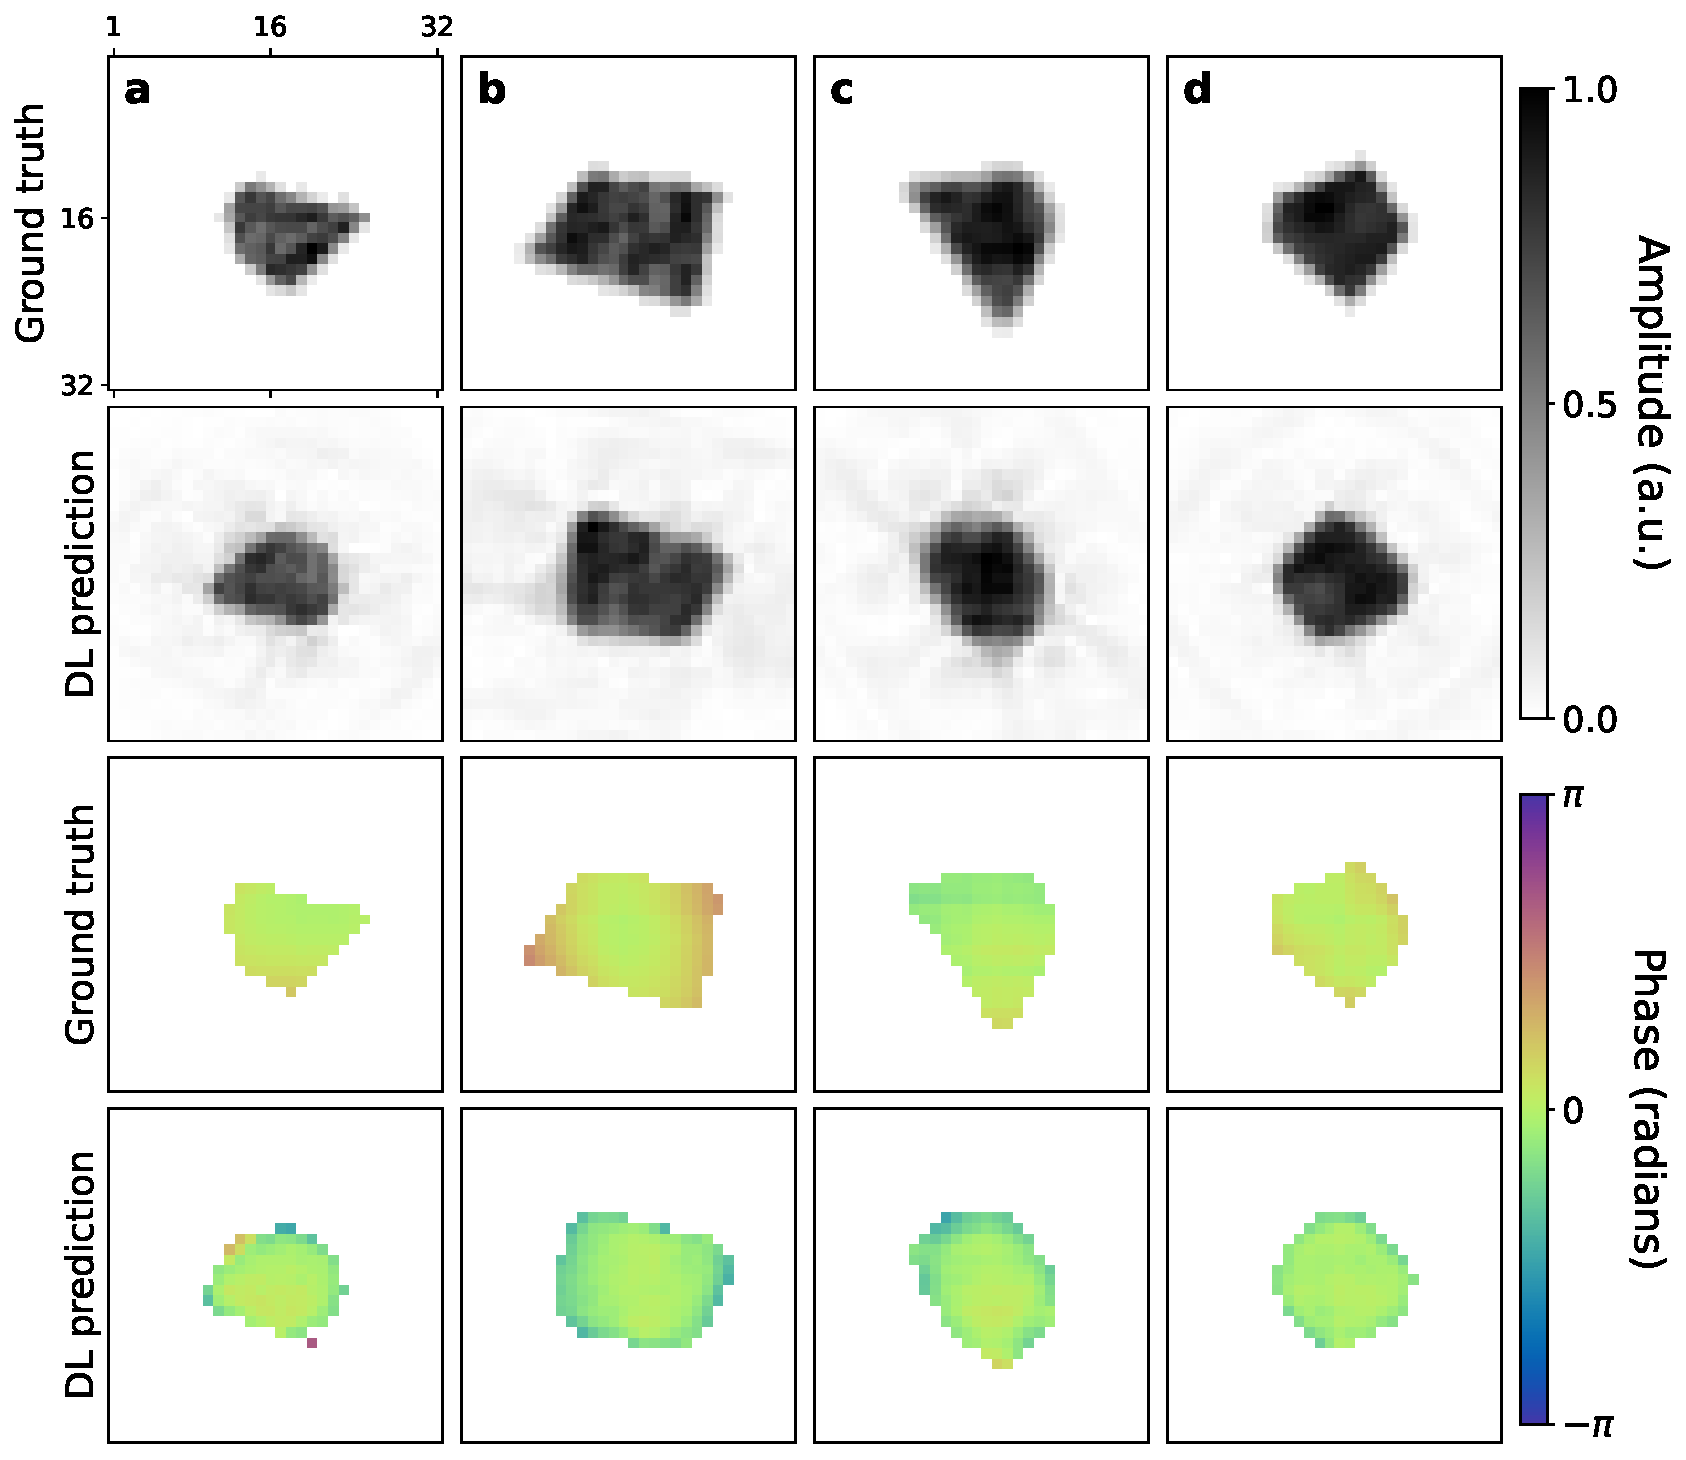
\includegraphics[width=.8\textwidth]{figures/Phasing/obj_low_strain_VFN.pdf}
    \caption{\textbf{Corresponding reconstructed objects}. Ground truth and predicted objects' amplitudes (first two rows 
    respectively) and ground truth and predicted objects' phases (first two rows respectively). }
    \label{fig:obj_vfn}
\end{figure}

The results obtained from the model trained with the WCA loss function are visually better than the MSE ones. Although not 
completely removed, the sign symmetry that gives rise to the superposition of the object with its twin, is less pronounced. 
For example, particles in Fig. \ref{fig:obj_vfn}(a-b-d) have a clear orientation and a shape that matches the ground truth. 
In all those cases though, the model has opted for the conjugate solution as the predicted object are flipped with respect to 
the ground truth ones. In Fig. \ref{fig:obj_vfn}(c) instead the symmetry is not broken and the result is still a superposition 
of the particle with its twin. This suggests that the symmetry breaking method implemented in the WCA, and the one proposed by 
Zhang and coauthors, is only partially playing a role in the actual model learning. It is interesting to notice indeed that 
when the training dataset or the model trainable parameters are increased, the sign symmetry is completely removed in the most 
difficult cases as well. Fig. \ref{fig:loss_comparison} shows the effect of the dataset and models sizes for both MSE and WCA 
loss functions on the same simulated test data. The first important piece of information this figure shows is that the model trained 
with the WCA reaches higher accuracy. Moreover, it is much faster to compute since no FFT or IFFT is involved, thus the training time 
is drastically reduced. For what concerns the accuracy metric, in order to properly account for both modulus and phase, 
it has been calculated using 
\begin{equation}
 \left(\frac{PCC(m) + WCA(\varphi)}{2}\right)\times 100
\end{equation}
where $PCC(m)$ is the Pearson Correlation Coefficient on the object's modulus and $WCA(\varphi)$ is the WCA function 
applied to the object's phase inside the support. For what concerns the sign symmetry problem it is evident that while for 
the MSE trained model it is resolved only for a larger number of trainable parameters, for the WCA trained one it is already 
sufficiently overcome. As last observation, it is interesting to notice that when the model size is kept fixed and the training 
dataset augmented, the WCA improves the performances while for the MSE it is not the case. 

\begin{figure}[H]
    \centering
    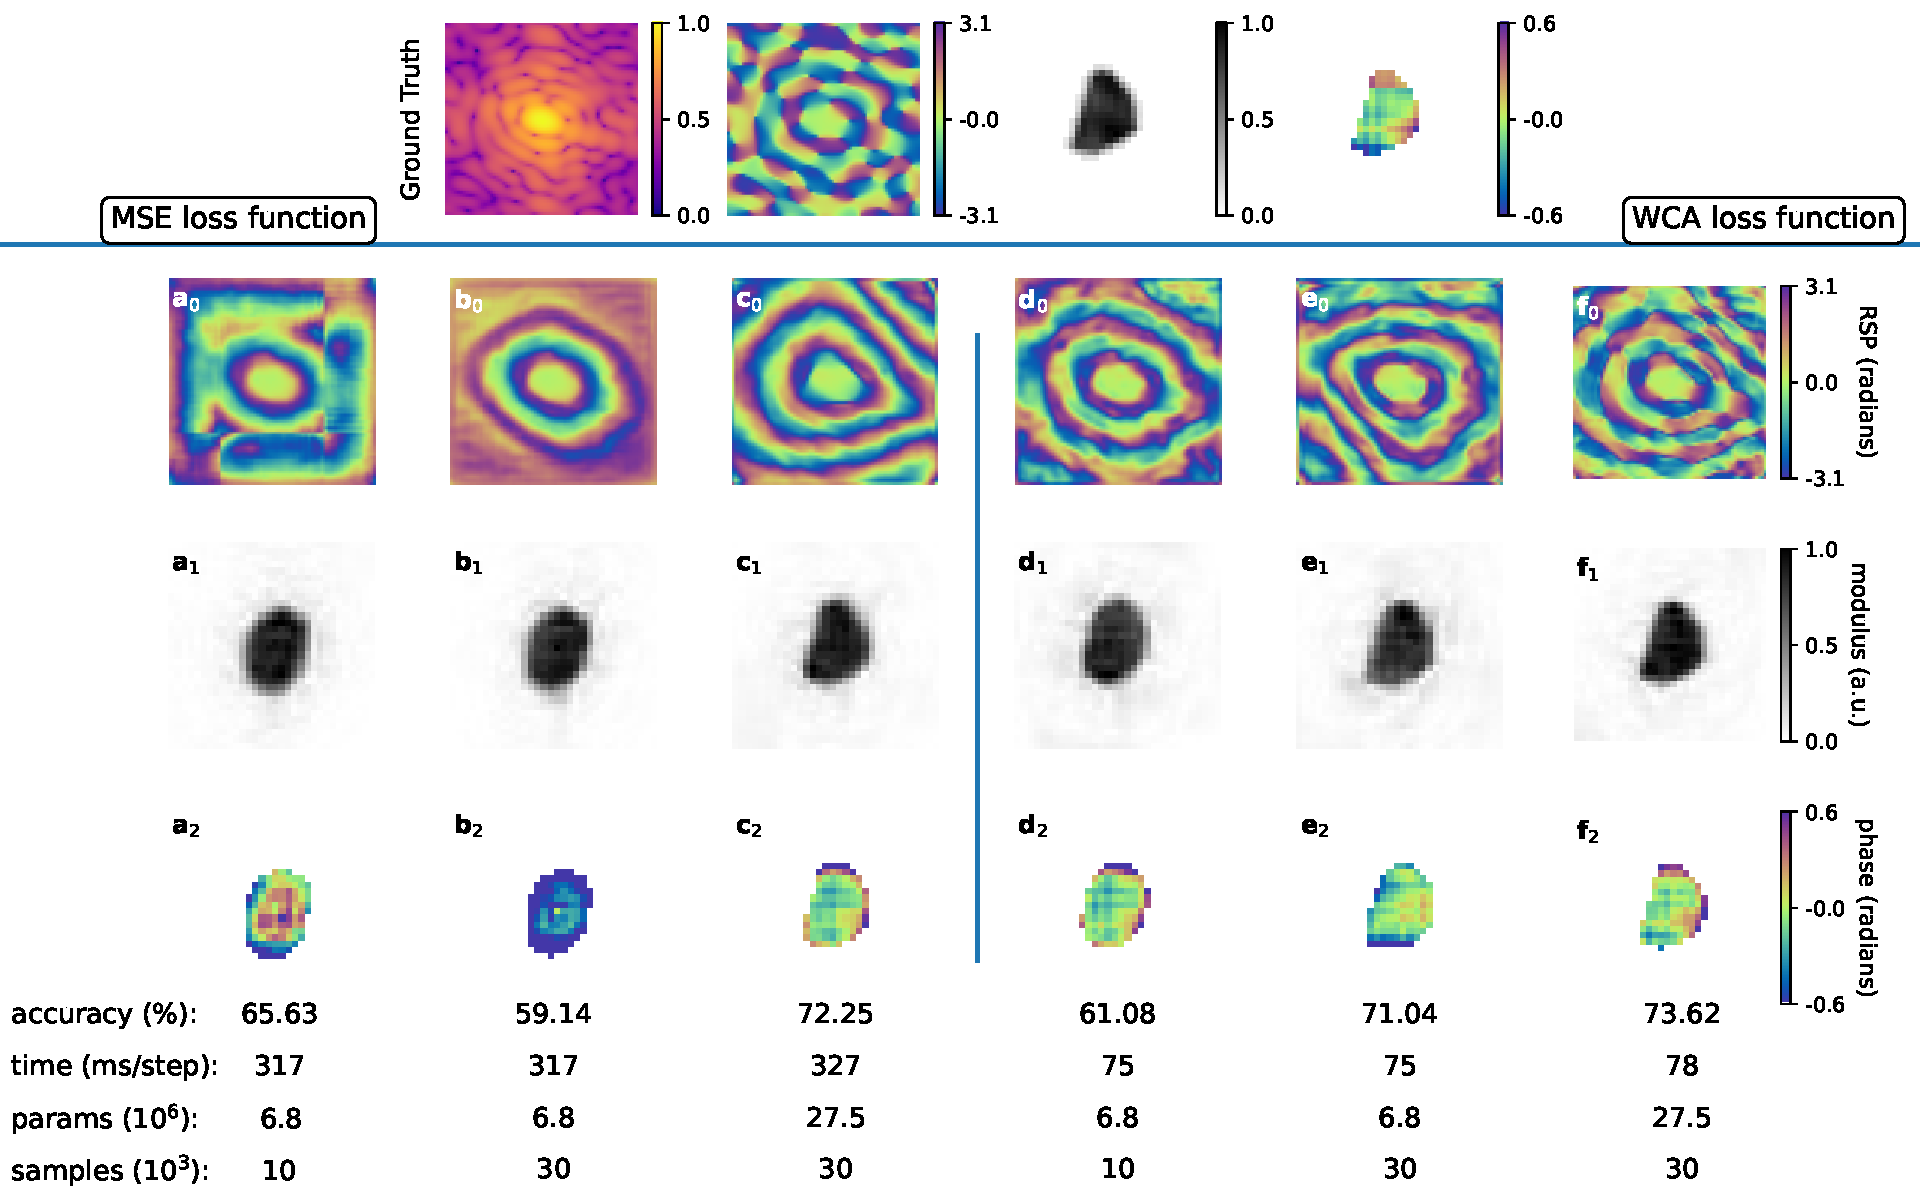
\includegraphics[width=\textwidth]{figures/Phasing/model_comparison.pdf}
    \caption{\textbf{Comparison of MSE and WCA loss function for different model and training dataset sizes} In the first 
    row from left to right the input intensity, the ground truth RSP and the corresponding object (modulus and phase) are 
    represented. \textbf{$a_0, b_0, c_0$}} are the results of the predicted RSP obtained from the model trained with the 
    MSE loss function with the initial number of parameters and training set (\textbf{a}), with the augmented dataset (\textbf{b})
    and with both model and dataset size increased (\textbf{c}) In third and fourth rows the corresponding reconstructed 
    objects are displayed. \textbf{$d, e, f$} columns symmetrically shows the results obtained with the model trained using the WCA loss. 
    \label{fig:loss_comparison}
\end{figure}

\section{2D high strain case}

In this paragraph the model training was performed on a dataset of highly strained 2D BCDI pattern simulated as described above  
in section \ref{sec:dataset_creation2D}. In this case Poisson statistic was applied to each dataset to better simulate 
the experimental condition. A set containing 30'000 samples was created and the ``bigger'' model of 27.5M parameters mentioned in Fig 
\ref{fig:loss_comparison} was trained over 50 epochs with a learning rate of 0.001. Similarly to the low-strain case 
described above the same model has been trained with the MSE and WCA losses separately for comparison. The goal of this 
study is in fact to test the relevance of the loss function compared to the size of the model when the complexity of the 
task increases. The results on 4 test BCDI pattern are shown in Figs. \ref{fig:2D_hs_MSE_RSP}-\ref{fig:2D_hs_MSE_obj} for the MSE
one and \ref{fig:2D_hs_VFN_obj}-\ref{fig:2D_hs_VFN_obj} for the WCA.

\begin{figure}[H]
    \centering
    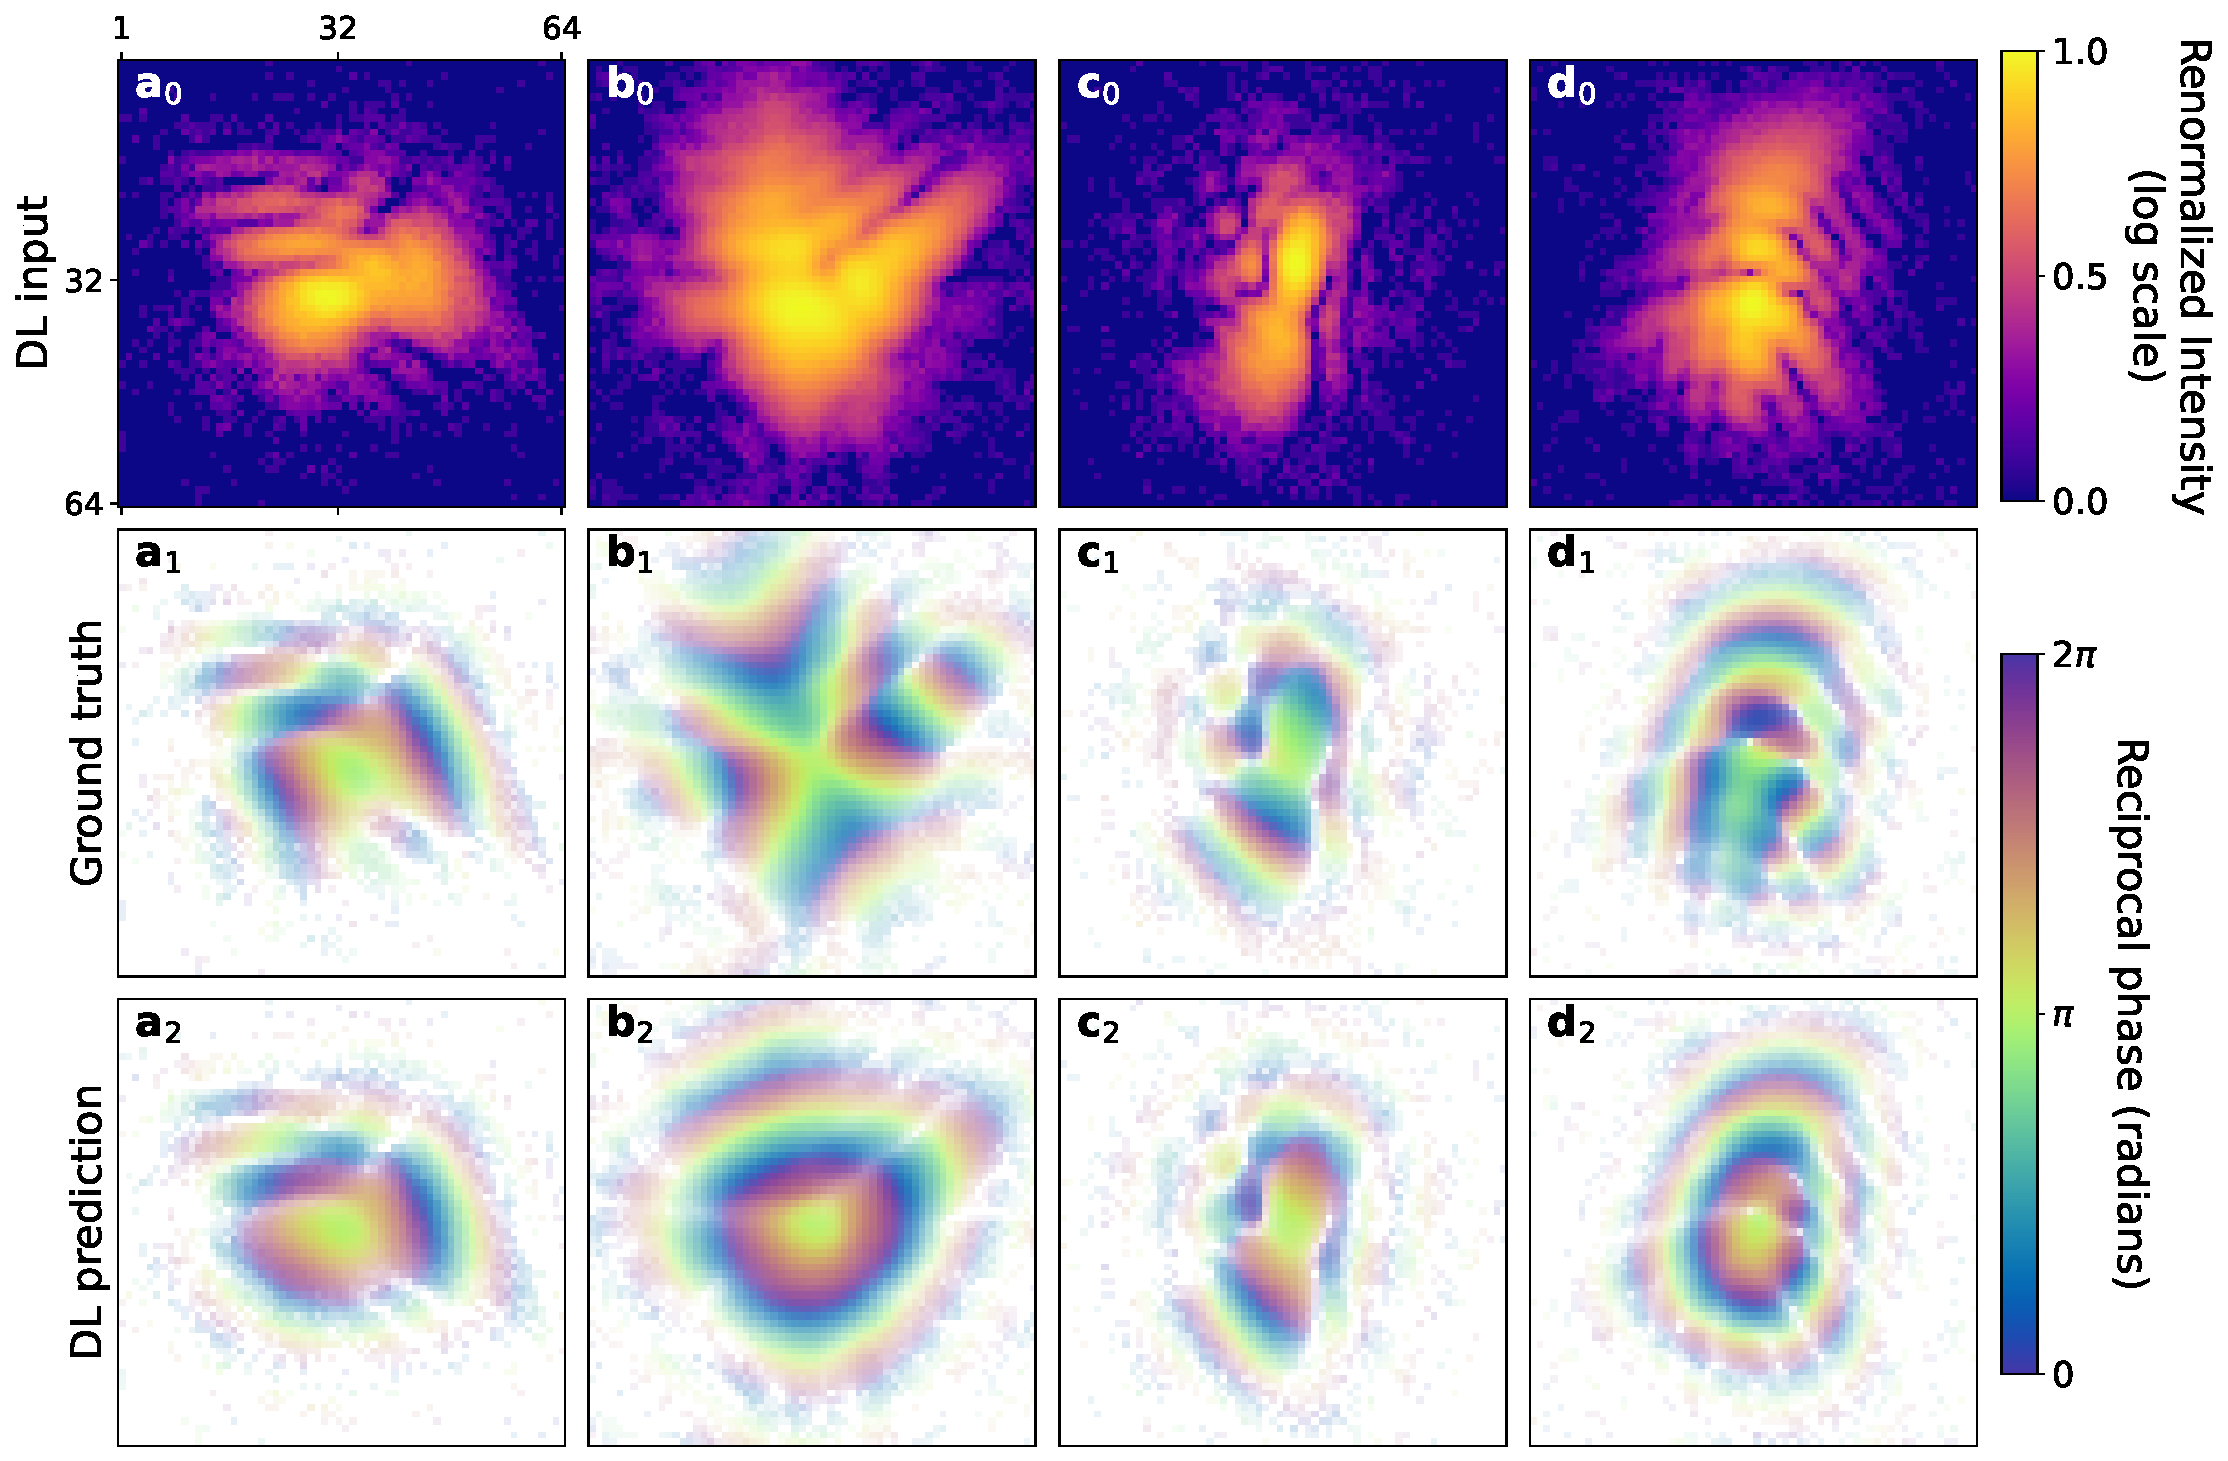
\includegraphics[width=\textwidth]{figures/Phasing/2D_hs_MSE_RSP.pdf}
    \caption{RSP predicted by the model trained with the MSE loss function calculated on both modulus and phase of the 
    reconstructed object. First row: simulated 2D strained BCDI patterns (test dataset). Second row: 
    corresponding ground truth RSP. Third row: predicted RSP. Once can notice that the model cannot predict correctly the 
    RSP where the ``iso-phases'' do not have a circular symmetry (see \textbf{b-d}).} 
    \label{fig:2D_hs_MSE_RSP}
\end{figure}

\begin{figure}[H]
    \centering
    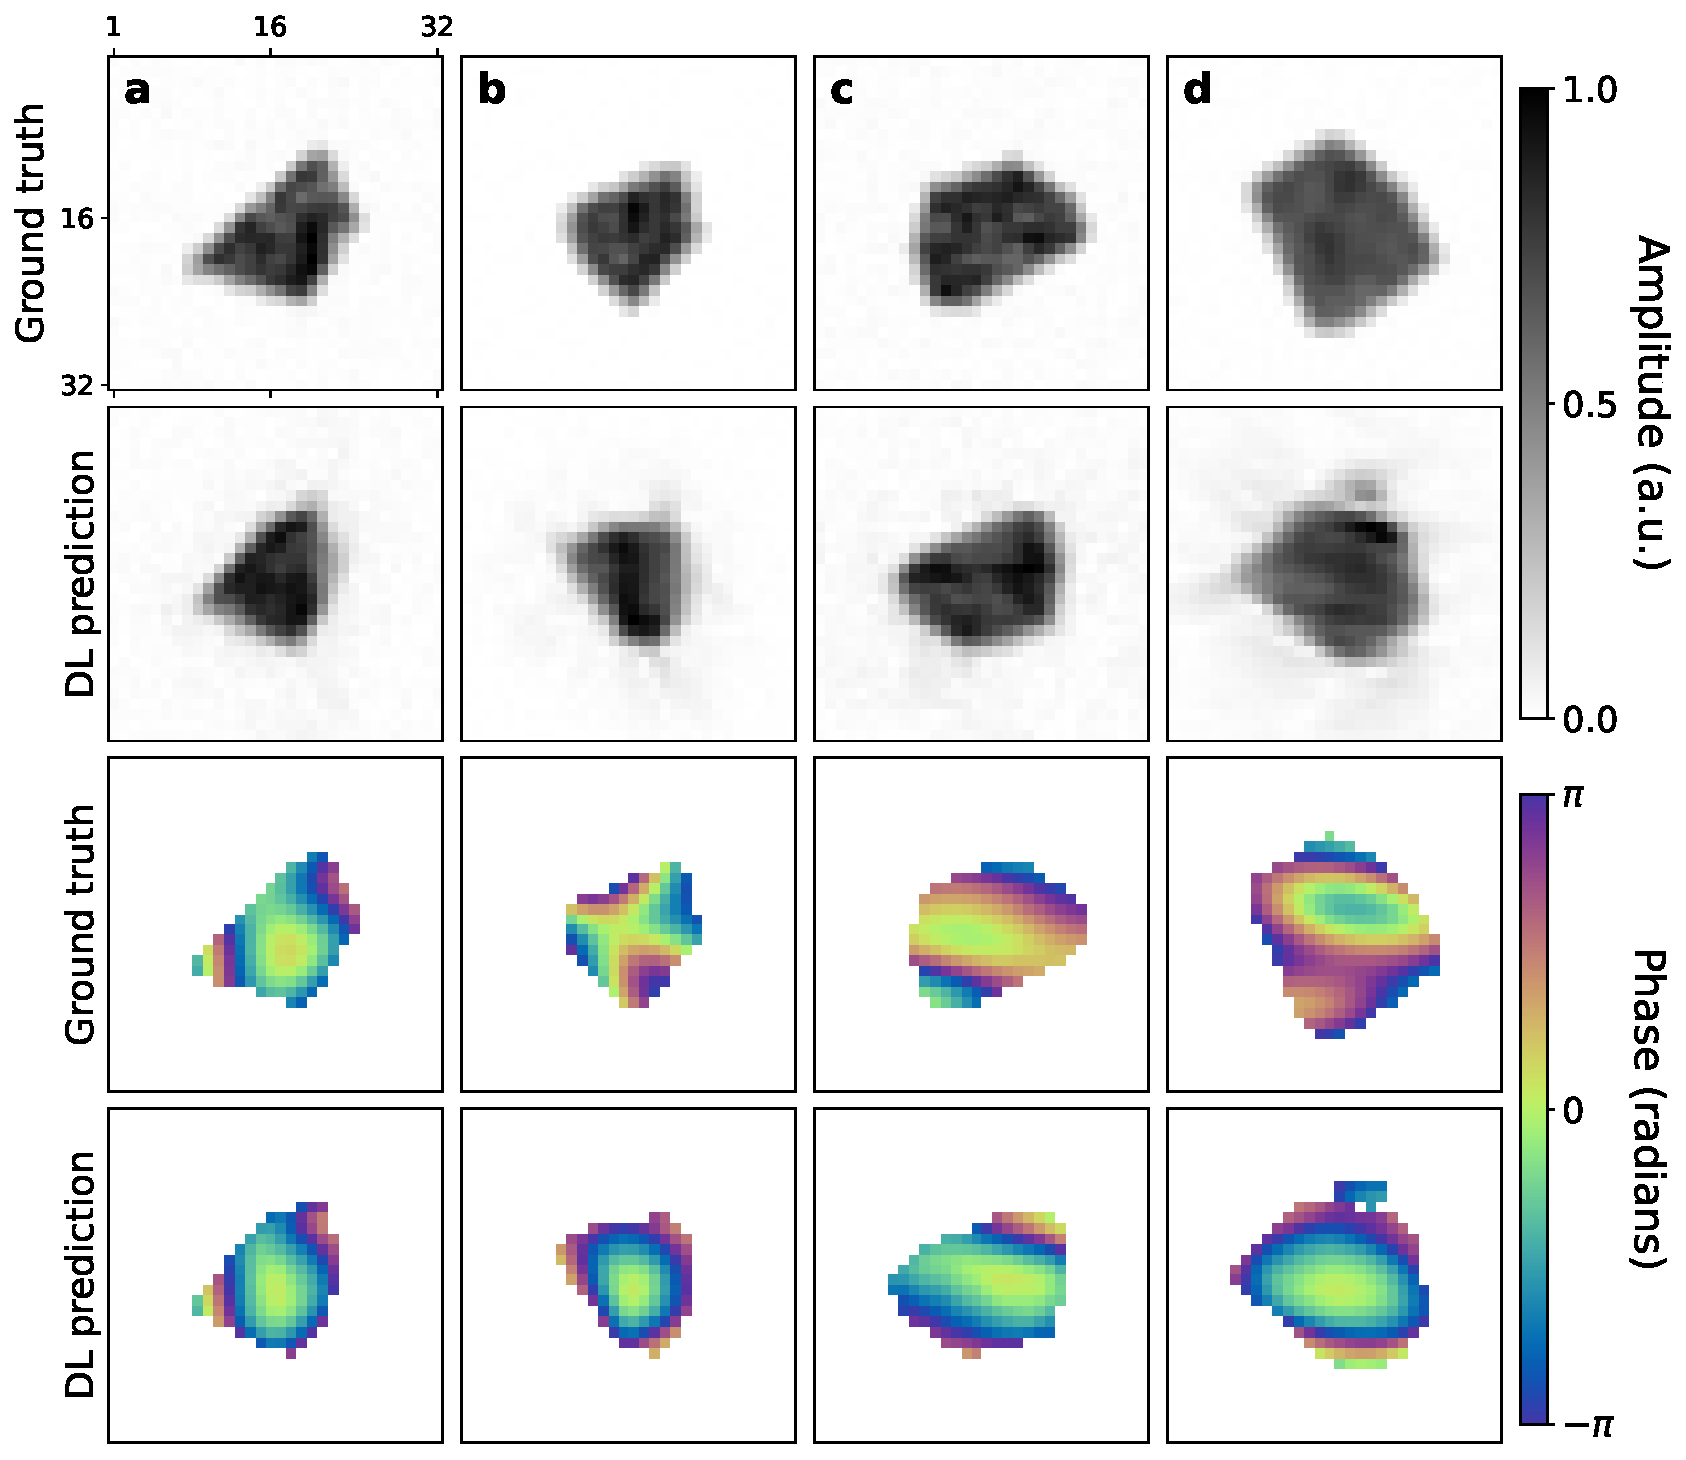
\includegraphics[width=\textwidth]{figures/Phasing/2D_hs_MSE_obj.pdf}
    \caption{Corresponding reconstructed objects. First and third row: ground truth modulus and phase. Second and fourth row: 
    model's results of objects' modulus and phase. Although the shape might at first sight look like the ground truth one (or 
    the twin) the phase is often incorrect. It is curious to notice that better results are obtained when the object's 
    phase possesses a certain degree of symmetry with respect to the center, analogously to the corresponding RSP. } 
    \label{fig:2D_hs_MSE_obj}
\end{figure}

\begin{figure}[H]
    \centering
    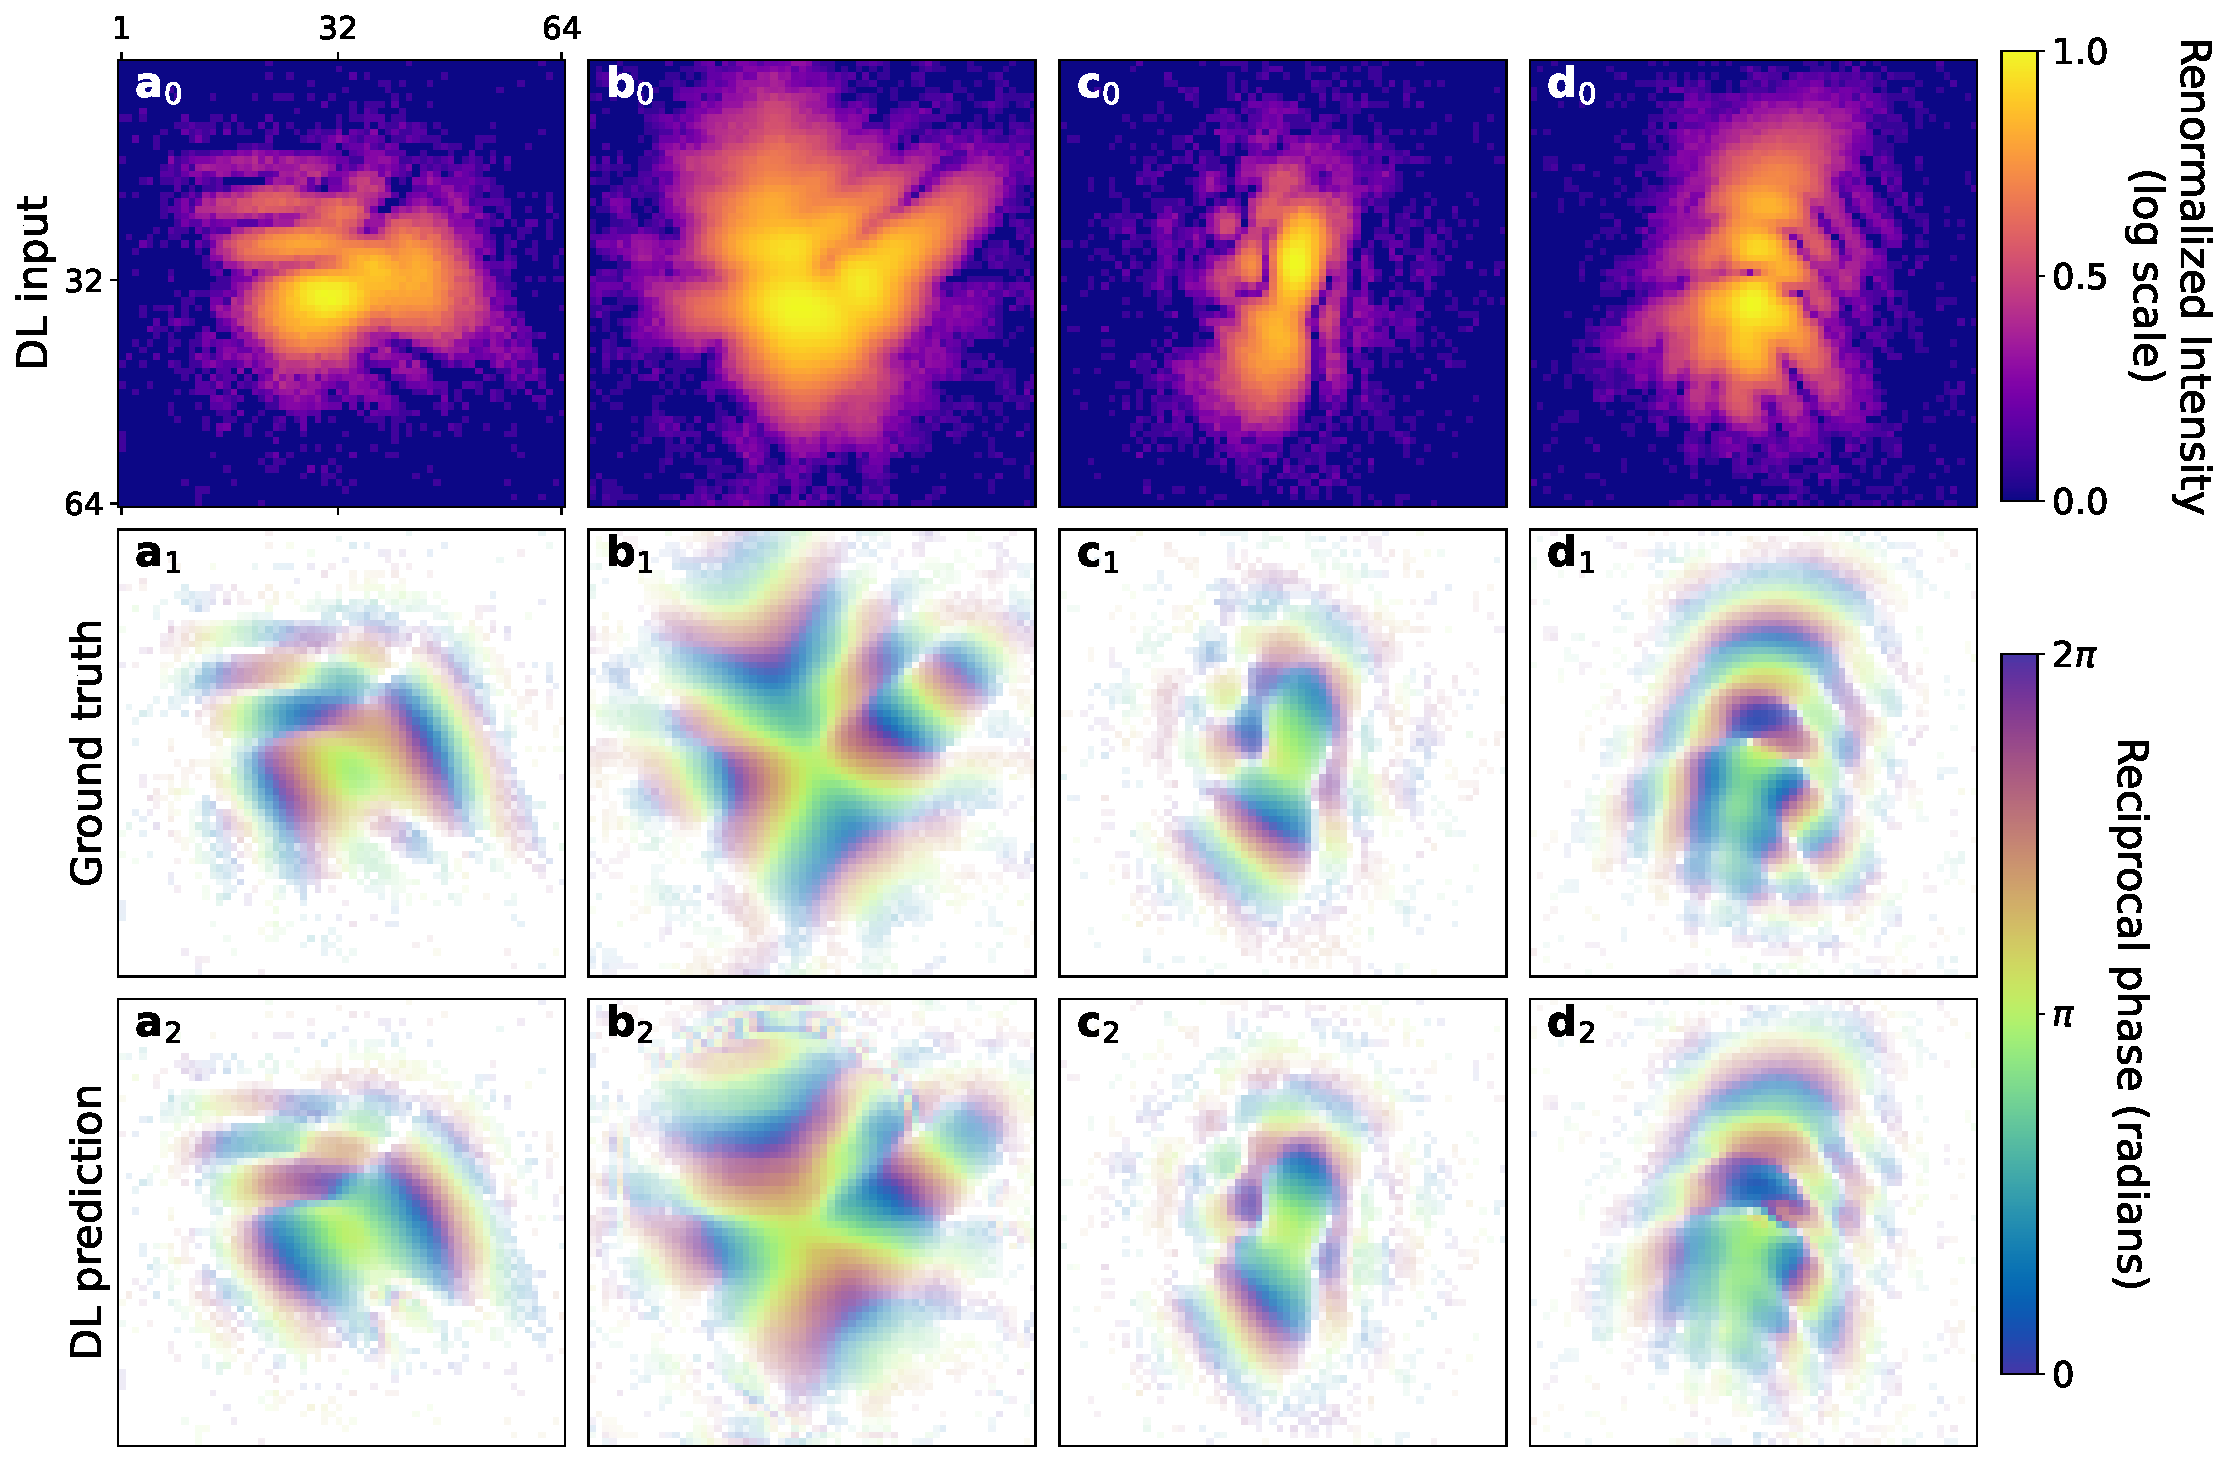
\includegraphics[width=\textwidth]{figures/Phasing/2D_hs_VFN_RSP.pdf}
    \caption{RSP predicted by the model trained with the WCA loss function. Here the model correctly retrieves the RSP for 
    non-circularly symmetric structures as well (\textbf{b-d})} 
    \label{fig:2D_hs_VFN_RSP}
\end{figure}

\begin{figure}[H]
    \centering
    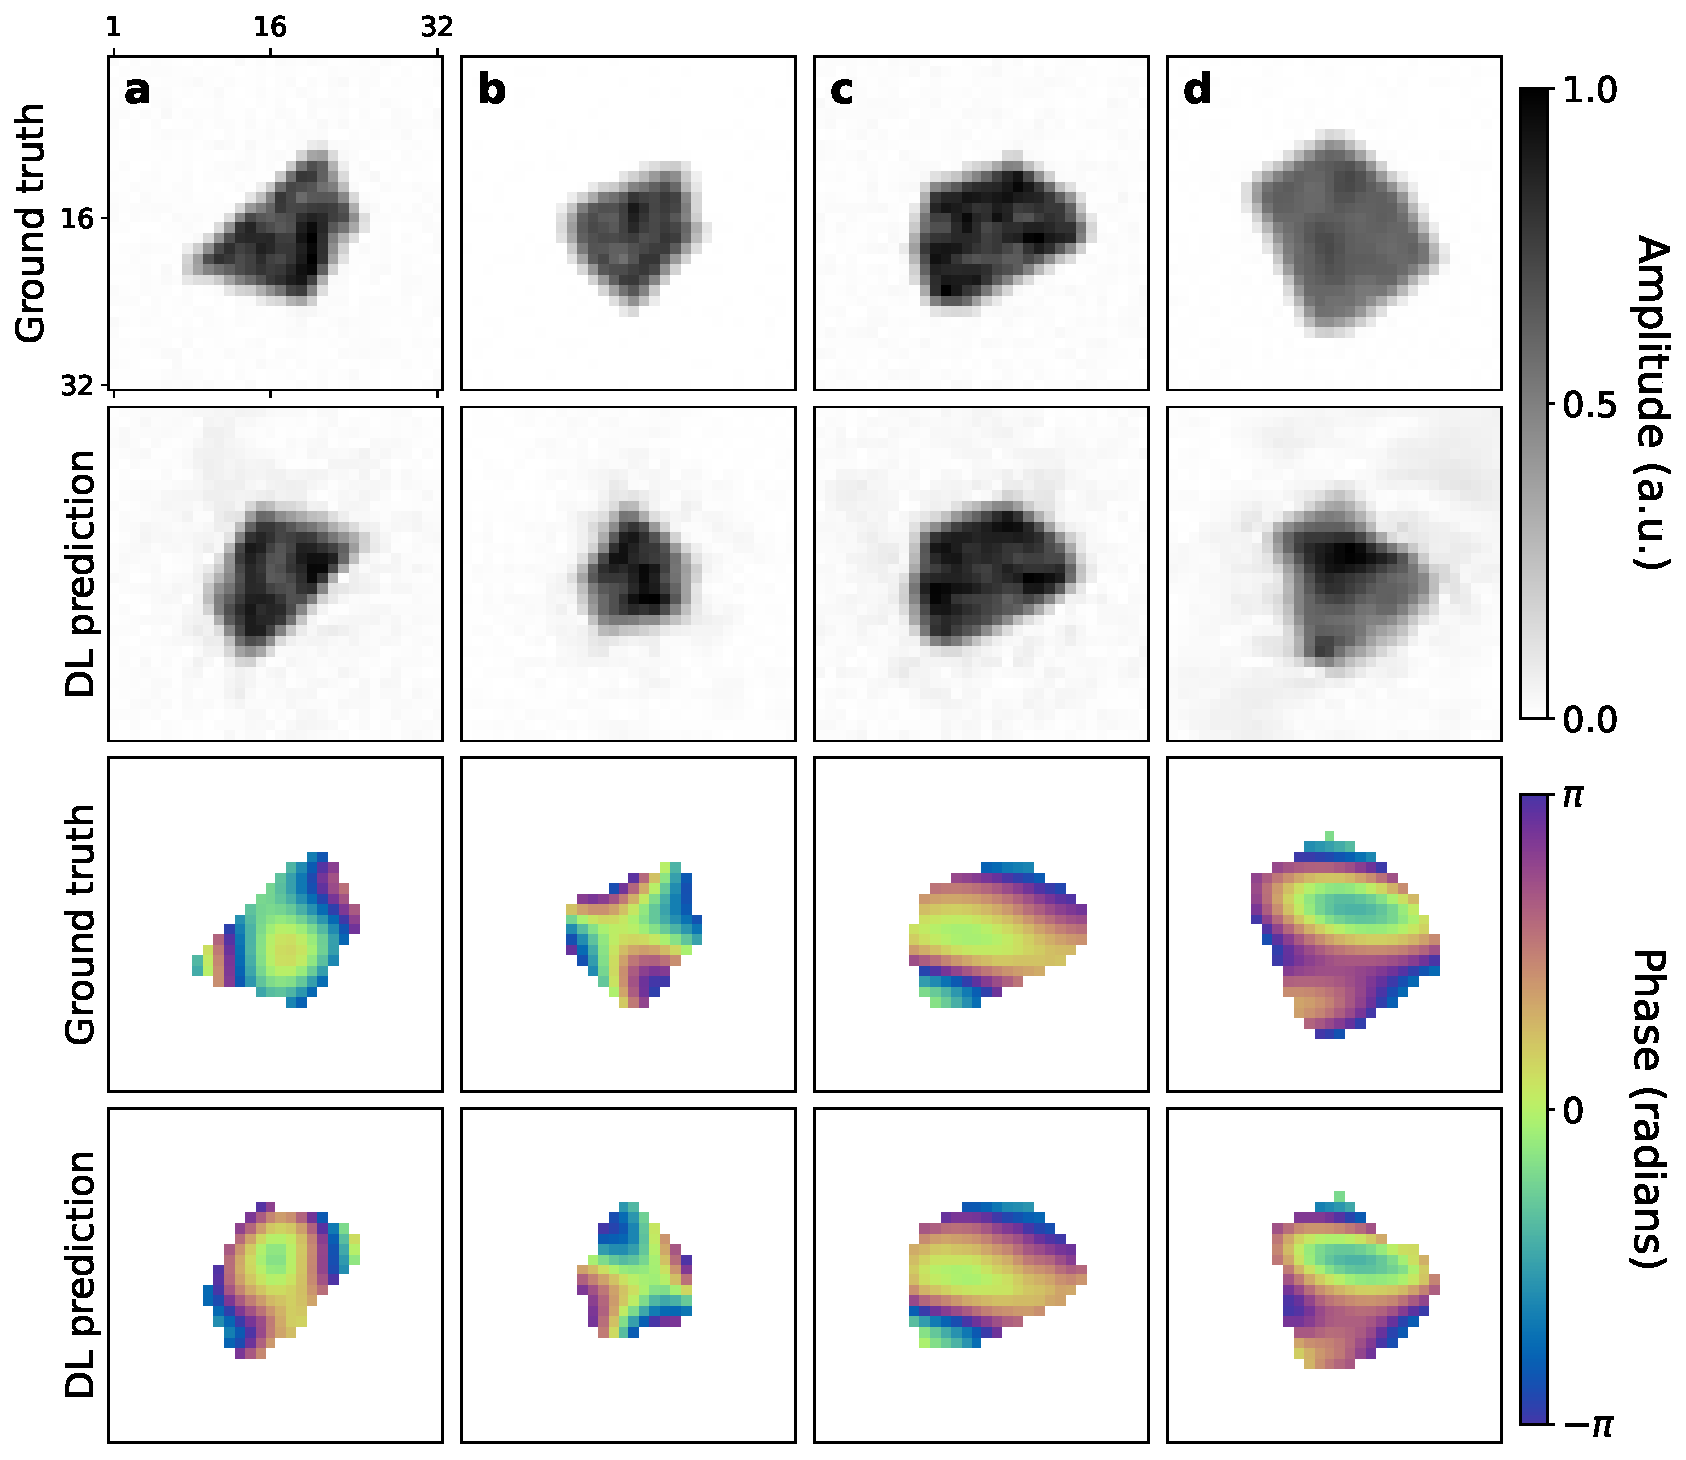
\includegraphics[width=\textwidth]{figures/Phasing/2D_hs_VFN_obj.pdf}
    \caption{Corresponding reconstructed objects. Compared to Fig.\ref{fig:2D_hs_MSE_obj} the phase of the object is 
    correctly recovered.} 
    \label{fig:2D_hs_VFN_obj}
\end{figure}


The preliminary studies on the 2D case for low-strain particles have demonstrated the possibility to recover the RSP from 
the diffracted intensity pattern with a U-Net like architecture without ever calculating the object in real space. Moreover, 
the studies on the high strain particles has shown that this model configuration is well suited for this case as well.
From these promising results, it was decided to investigate the mapping intensity-RSP for portions of the reciprocal space. 


\section{Phasing patches: 3D case low strain}\label{chp:patches_nostrain}
% MODEL 3D CASE NO STRAIN WITH PATCHES: SHOW THE MODEL WITH DIFFERENT WCA LOSS FUNCTION 
In this section of the manuscript the DL prediction of ``patches'' of the RSP will be explored and discussed. 
Three-dimensional BCDI pattern of low strained particles were used to conduct this study. 
Although this patching approach has not given satisfactory results for the PR, it is nevertheless reported in the manuscript as 
study on the \textit{local} rather than \textit{global} relationship between the diffracted intensity and the RSP. It is 
indeed known that there exist a unique mapping, barring some trivial RSP symmetries, between the diffracted intensity 
and the RSP in 3D \cite{Miao:98}. What is interesting to investigate is whether this relationship exists also for subsets 
of the reciprocal space, and in particular if it can be retrieved by a DL model. (From now on the term ``patches'' 
will be used to refer to cubic subsets of the reciprocal space). \\

When deciding to work with patches, there is a number of questions that arise and the answer to which is not 
straightforward nor unique in many cases. Namely: What size is best? Can the patches 
be extracted at random positions or should there be an order? What about the normalization of the intensity range inside 
the patch? How are the patches stitched together into the full RSP eventually? How are the phase symmetries taken into account 
during the stitching? 
Here I will present the approach that allowed me to address these questions. 

\subsection{The choice of the size}

Similarly to the inpainting case, 32 pixel-side cubic patches, cropped out of 128 pixel-side simulated
BCDI patterns were considered. The choice is supported by the following reasons: 

\begin{itemize}
    \item The good results obtained for the inpainting case suggested that the amount of information contained inside a
    32 pixel-side patch of reciprocal space is enough for the model to grasp spatial correlations.  
    \item The average oversampling ratio of BCDI experimental data is such that in a 32 pixel-side volume a sufficient
    amount of fringes is contained, meaning intuitively that the model can predict the corresponding RSP. 
    \item An even number multiple of 2 is usually considered GPU-friendly since it facilitates the shared calculations across
    different threads. 
\end{itemize}

\subsection{Patches division and stitching}\label{sbsec:patches_creation}
At first, the patches were thought to be extracted randomly from the full BCDI pattern as for the inpainting case. 
However, by doing so the RSP of each patch would in principle have different offsets and different wraps than the neighbors 
and this would complicate the stitching of the patches back into the full RSP. 
For this reason, and considering the approximate spherical symmetry of the average BCDI pattern it was decided to crop patches radially, 
starting from the region around the center of the Bragg peak and the progressively moving outwards to higher q-values. 
In this configuration, an integer step (10 pixels in our case) was chosen beforehand and the first patch around the center 
of the Bragg peak was selected together with all the patches centered in distances of integer multiples of the chosen step. 
Fig. \ref{fig:patches_cropping} shows a simplified schematic of the patches extraction. 
For the DL model training the patches of the intensity pattern need to be selected as well as the for the corresponding 
RSP for ground truth comparison. 


\begin{figure}[H]
    \centering
    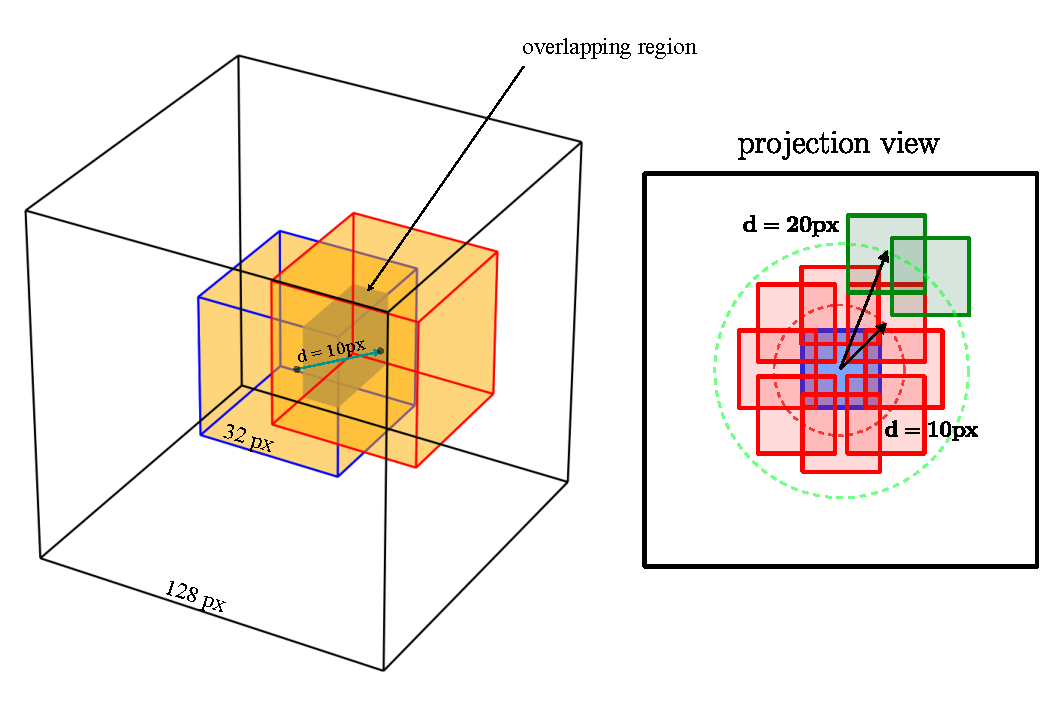
\includegraphics[width=\textwidth]{figures/Phasing/patching_cropping.pdf}
    \caption{Schematic of the cropping of patches. From the full BCDI pattern (white 128 px-sided cube) the first patch is 
    cropped out in the center and (orange 32 px-side cube with blue outline). Other patches are extracted radially from 
    concentric shells separated by a 10 pixels step. Here only one patch from the first shell at distance 10 pixels from the 
    center of the peak is displayed for simplicity. The gray shaded area highlights the overlapping volume between the 
    two patches. }
    
    \label{fig:patches_cropping}
\end{figure}

Being the step size smaller than the 
semi-diagonal of the 32 pixel-sided patches, it follows that the patches of adjacent cells have overlapping volumes. 
These common regions can have a twofold purpose. Firstly, they reduce the complexity of the stitching procedure since 
when this is executed progressively starting from the central patch, the sign and the offsets of the RSP are unambiguously 
fixed for all the following ones. Secondly, during the DL model training, for patches belonging to the outer shells, 
the overlapping volume of RSP belonging to the innermost adjacent shell can be provided as initial guess along with the input 
intensity patches. This of course cannot be exploited for the central patch that necessarily has to be predicted without 
initial RSP guesses. \\
The last question to be answered concerns the normalization. Since each patch is processed independently of the others 
by the DL model, it was decided to normalize each patch between 0 and 1 (always in log scale). 

To summarize, the final design implied the use of two distinct training datasets and two different CNNs. 
The first dataset was dedicated to the central portion, therefore the first CNN was provided with 3D intensity patches in 
input (normalized log scale) and corresponding RSP patches as ground truth labels. A second training dataset containing 
patches from outer shells (5 concentric ones for a 128 pixel-sided full BCDI pattern) was created. Here each file was made 
of the pair intensity-RSP initial guess - from the closest neighbor patch belonging to the innermost shell -  as input,
and the full RSP ground truth patch corresponding to the input intensity. This second dataset was used to train a second 
CNN identical to the first one. One observation regarding the datasets is that there is an intrinsic imbalance between the 
number of central patches and the outer ones. In fact, for a single full BCDI pattern, the number of patches in the first shell is 1, 
while the number of outer portions can go up to several hundreds. Moreover, the central patch is the most important one as it 
contains a low resolution representation of the particle in real space. In order to balance the training, the first dataset was 
augmented with more simulated data. 

\begin{figure}[H]
    \centering
    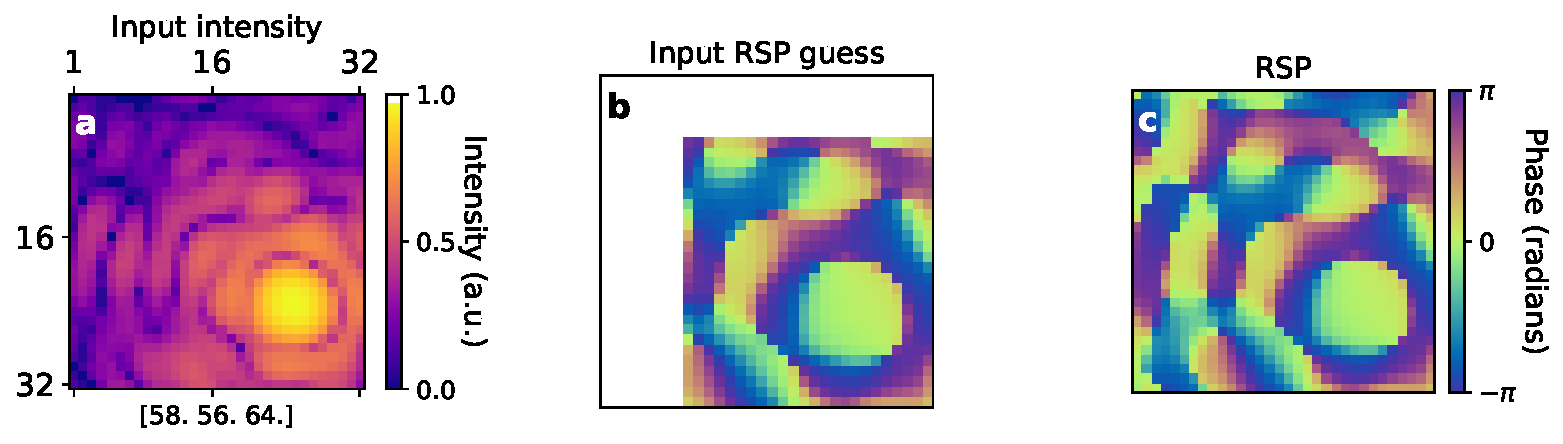
\includegraphics[width=\textwidth]{figures/Phasing/guess_RSP.pdf}
    \caption{Example of input-ground truth pairs for the outer patches model. \textbf{a} Central slice of the input intensity 
    for the patch cropped from the first shell at position [58,56,64] (the central patch is at [64,64,64]). \textbf{b} Initial 
    RSP guess deriving from the overlapping region of the intensity patch with the central one. The blank area represents 
    the part that needs to be predicted. \textbf{c} Ground truth RSP corresponding to the intensity patch in \textbf{a}.}
    
    \label{fig:patches_Xy}

\end{figure}

\subsection{Model architecture}\label{chp:3d_patch_model} 
The model architecture is similar to the one used for the inpainting case, with a U-Net like structure. 
5 encoder blocks reduce the feature map to 512 one-dimensional vectors in the bottleneck and 5 decoder blocks upsample 
the feature map back to the original size. Skip connections are used as well and similarly to the 2D case for Phase Retreival, 
the last layer has been left with no activation function. The total number of trainable parameters is of the order of 3.5 millions. \\
For the second CNN the layers and features are identical to the first one but three modifications were made. 
In particular, (i) the input tensor was composed of the intensity patch concatenated with the initial RSP guess and a binary 
mask marking the RSP guess voxels from the others. (ii) the mask was used at the exit of the decoder as well to 
select the new predicted voxels only for the backpropagation. 
(iii) The WCA loss function has been restricted only to the positive sign of the RSP since no sign ambiguity is left 
when fixing an initial guess. 

\subsection{Results on patches}

The first model has been trained over 50 epochs on 10'000 samples of central $32\times32\times32$ pixel-size patches 
cropped out of $128\times128\times128$ pixel-size full BCDI simulated pattern using the WCA loss function. 
Fig.\ref{fig:loss_3D_lowstrain} shows good learning curve which is supported by the results on test data, illustrated 
in Figs. \ref{fig:centralpatch_RSP_lowstrain} - \ref{fig:centralpatch_obj_lowstrain}

\begin{figure}[H]
    \centering
    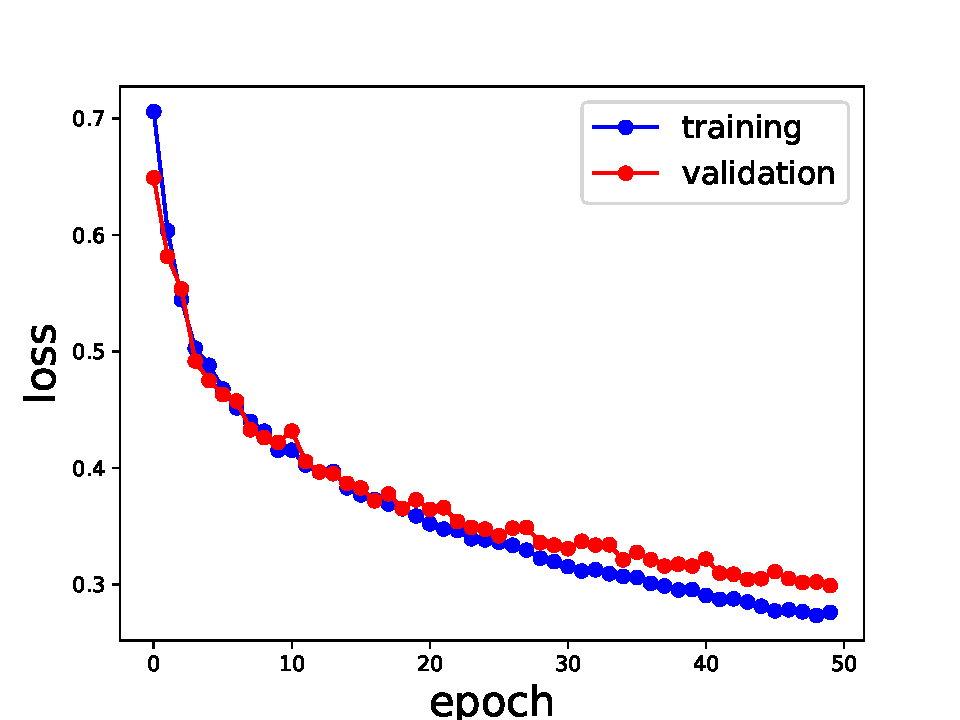
\includegraphics[width=\textwidth]{figures/Phasing/loss_central_patch.pdf}
    \caption{Training and validation loss curves over the 50 epochs long training. The plots indicate a good learning 
    of the model.}
    
    \label{fig:loss_3D_lowstrain}

\end{figure}

\begin{figure}[H]
    \centering
    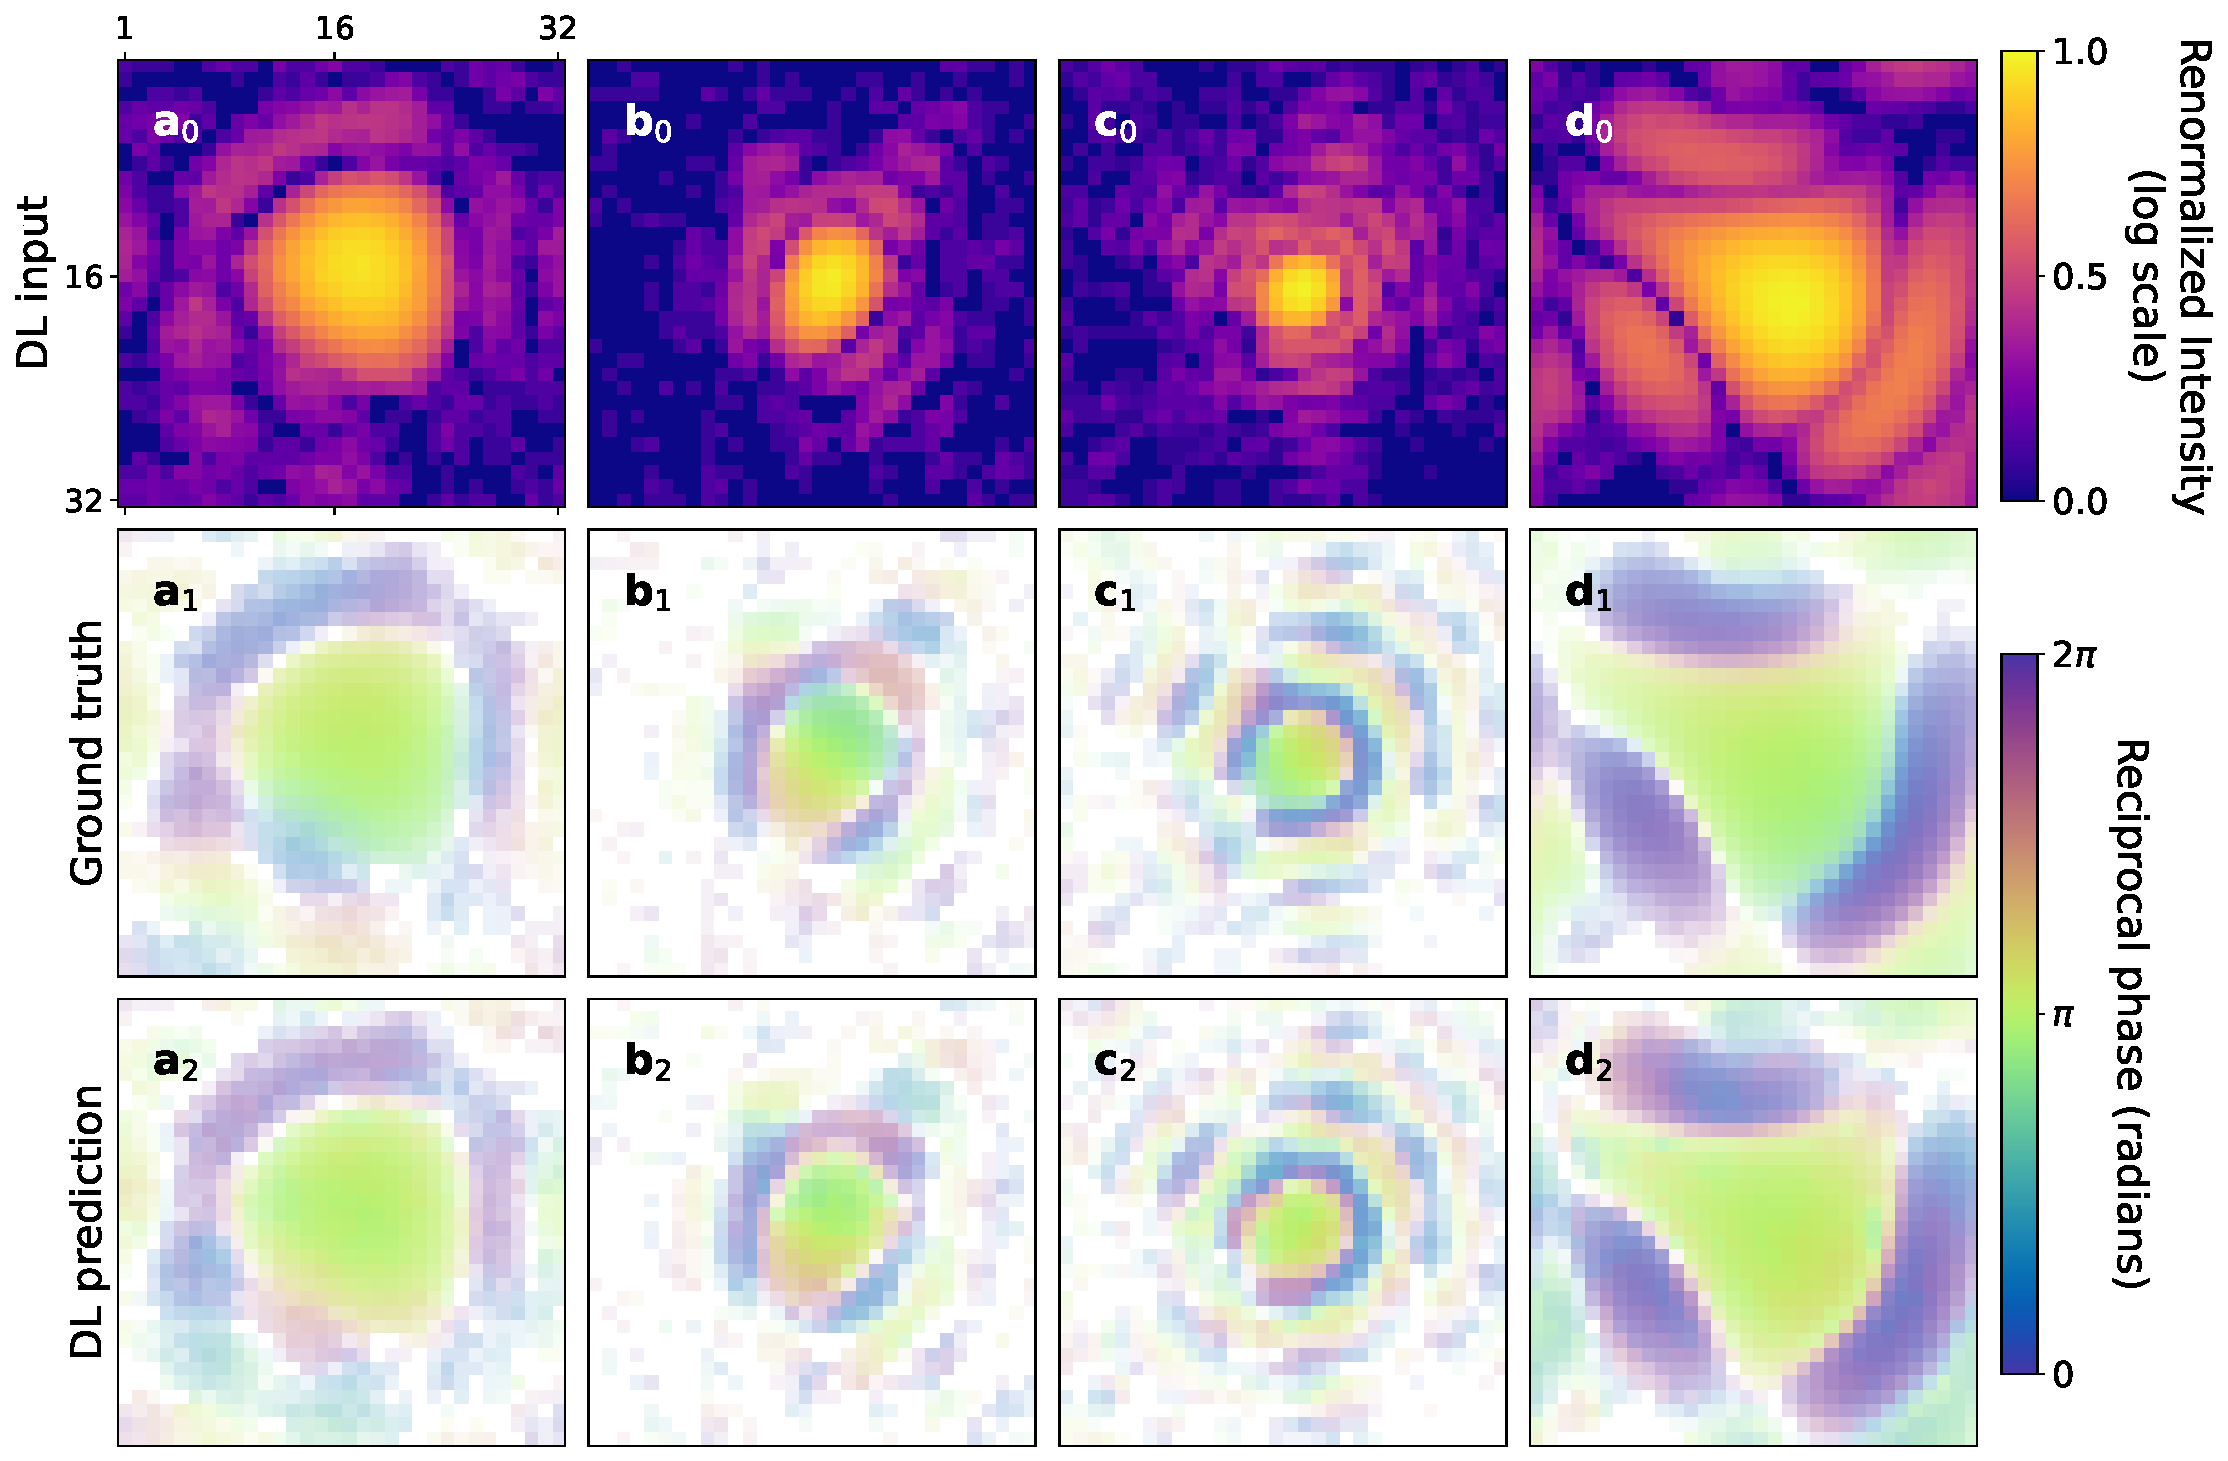
\includegraphics[width=\textwidth]{figures/Phasing/central_patch_lowstrain_RSP.pdf}
    \caption{Slices of the central patches. First row shows four different examples of BCDI patterns cropped around the 
    center of the peak. The small oversampling ratio of $\mathbf{b}_0$ and $\mathbf{b}_1$ makes such that the central portion 
    already contains the full useful signal and shows the diversity of the dataset. Row from $\mathbf{a}_1$ to $\mathbf{d}_1$
    shows the corresponding ground truth RSP while the last row shows the RSP predicted by the DL model.  }
    
    \label{fig:centralpatch_RSP_lowstrain}

\end{figure}
\begin{figure}[H]
    \centering
    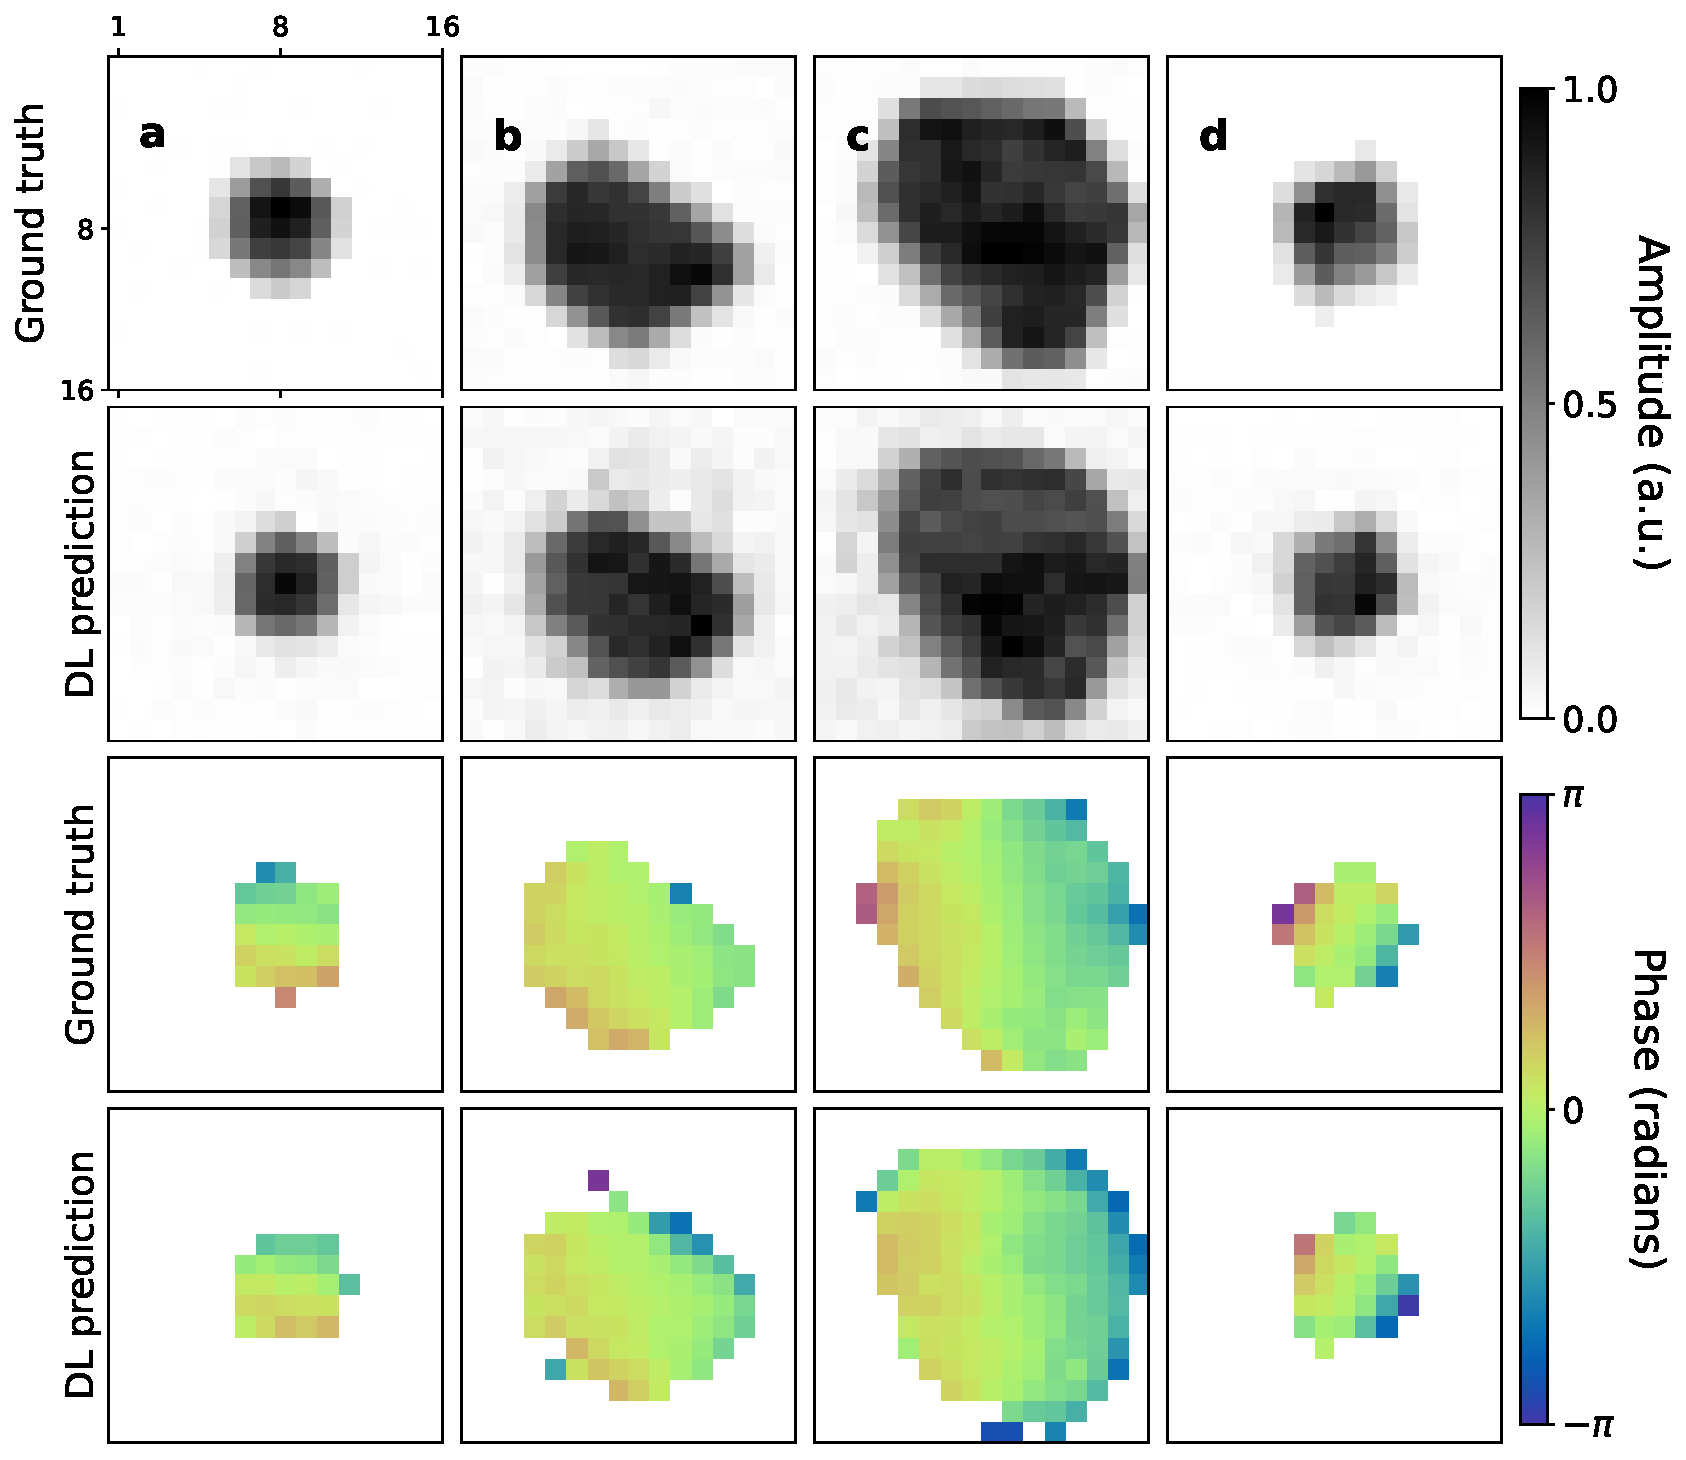
\includegraphics[width=\textwidth]{figures/Phasing/central_patch_lowstrain_obj.pdf}
    \caption{Corresponding objects. First and third rows show the modulus and the phase of the ground truth objects while
    second and fourth rows show the predicted ones. Although the low resolution due to the limited reciprocal space window, 
    the model proves to correctly find the shape and phase distribution of the particle. }

    \label{fig:centralpatch_obj_lowstrain}
\end{figure}

From the results obtained after the training of the model dedicated to the central portion of the simulated BCDI patterns, 
one can conclude that the model is capable of retrieving the correct RSP for the low strain case, meaning that the leap from 
the 2D case to the 3D case does not imply unforeseen complications. Moreover, given the diversity of the training dataset 
the model manages successfully for full peaks contained in a small patch. \\

The second CNN was trained on patches extracted from outer shells over 50 epochs on a dataset containing 50'000 samples. 
Fig. \ref{fig:outerpatch_obj_lowstrain} illustrates some relevant results. In particular one can observe that the model 
can predict the RSP in the missing regions providing a relatively smooth transition between the ``known'' and ``unknown''
parts. This result is particularly interesting as it proves that a CNN trained with the WCA loss function 
learn the map that links a portion of diffracted signal with the corresponding RSP with no information on the particle in
real space nor the position of this portion with respect to the center of the diffraction peak. It also shows that the 
size of the patches is contains a sufficient amount of information for this map to be learned. 
However, one can also notice that some ``noise'' is present in the predicted regions. These discrepancies from the ground 
truth become detrimental during the stitching procedure. 

\begin{figure}[H]
    \centering
    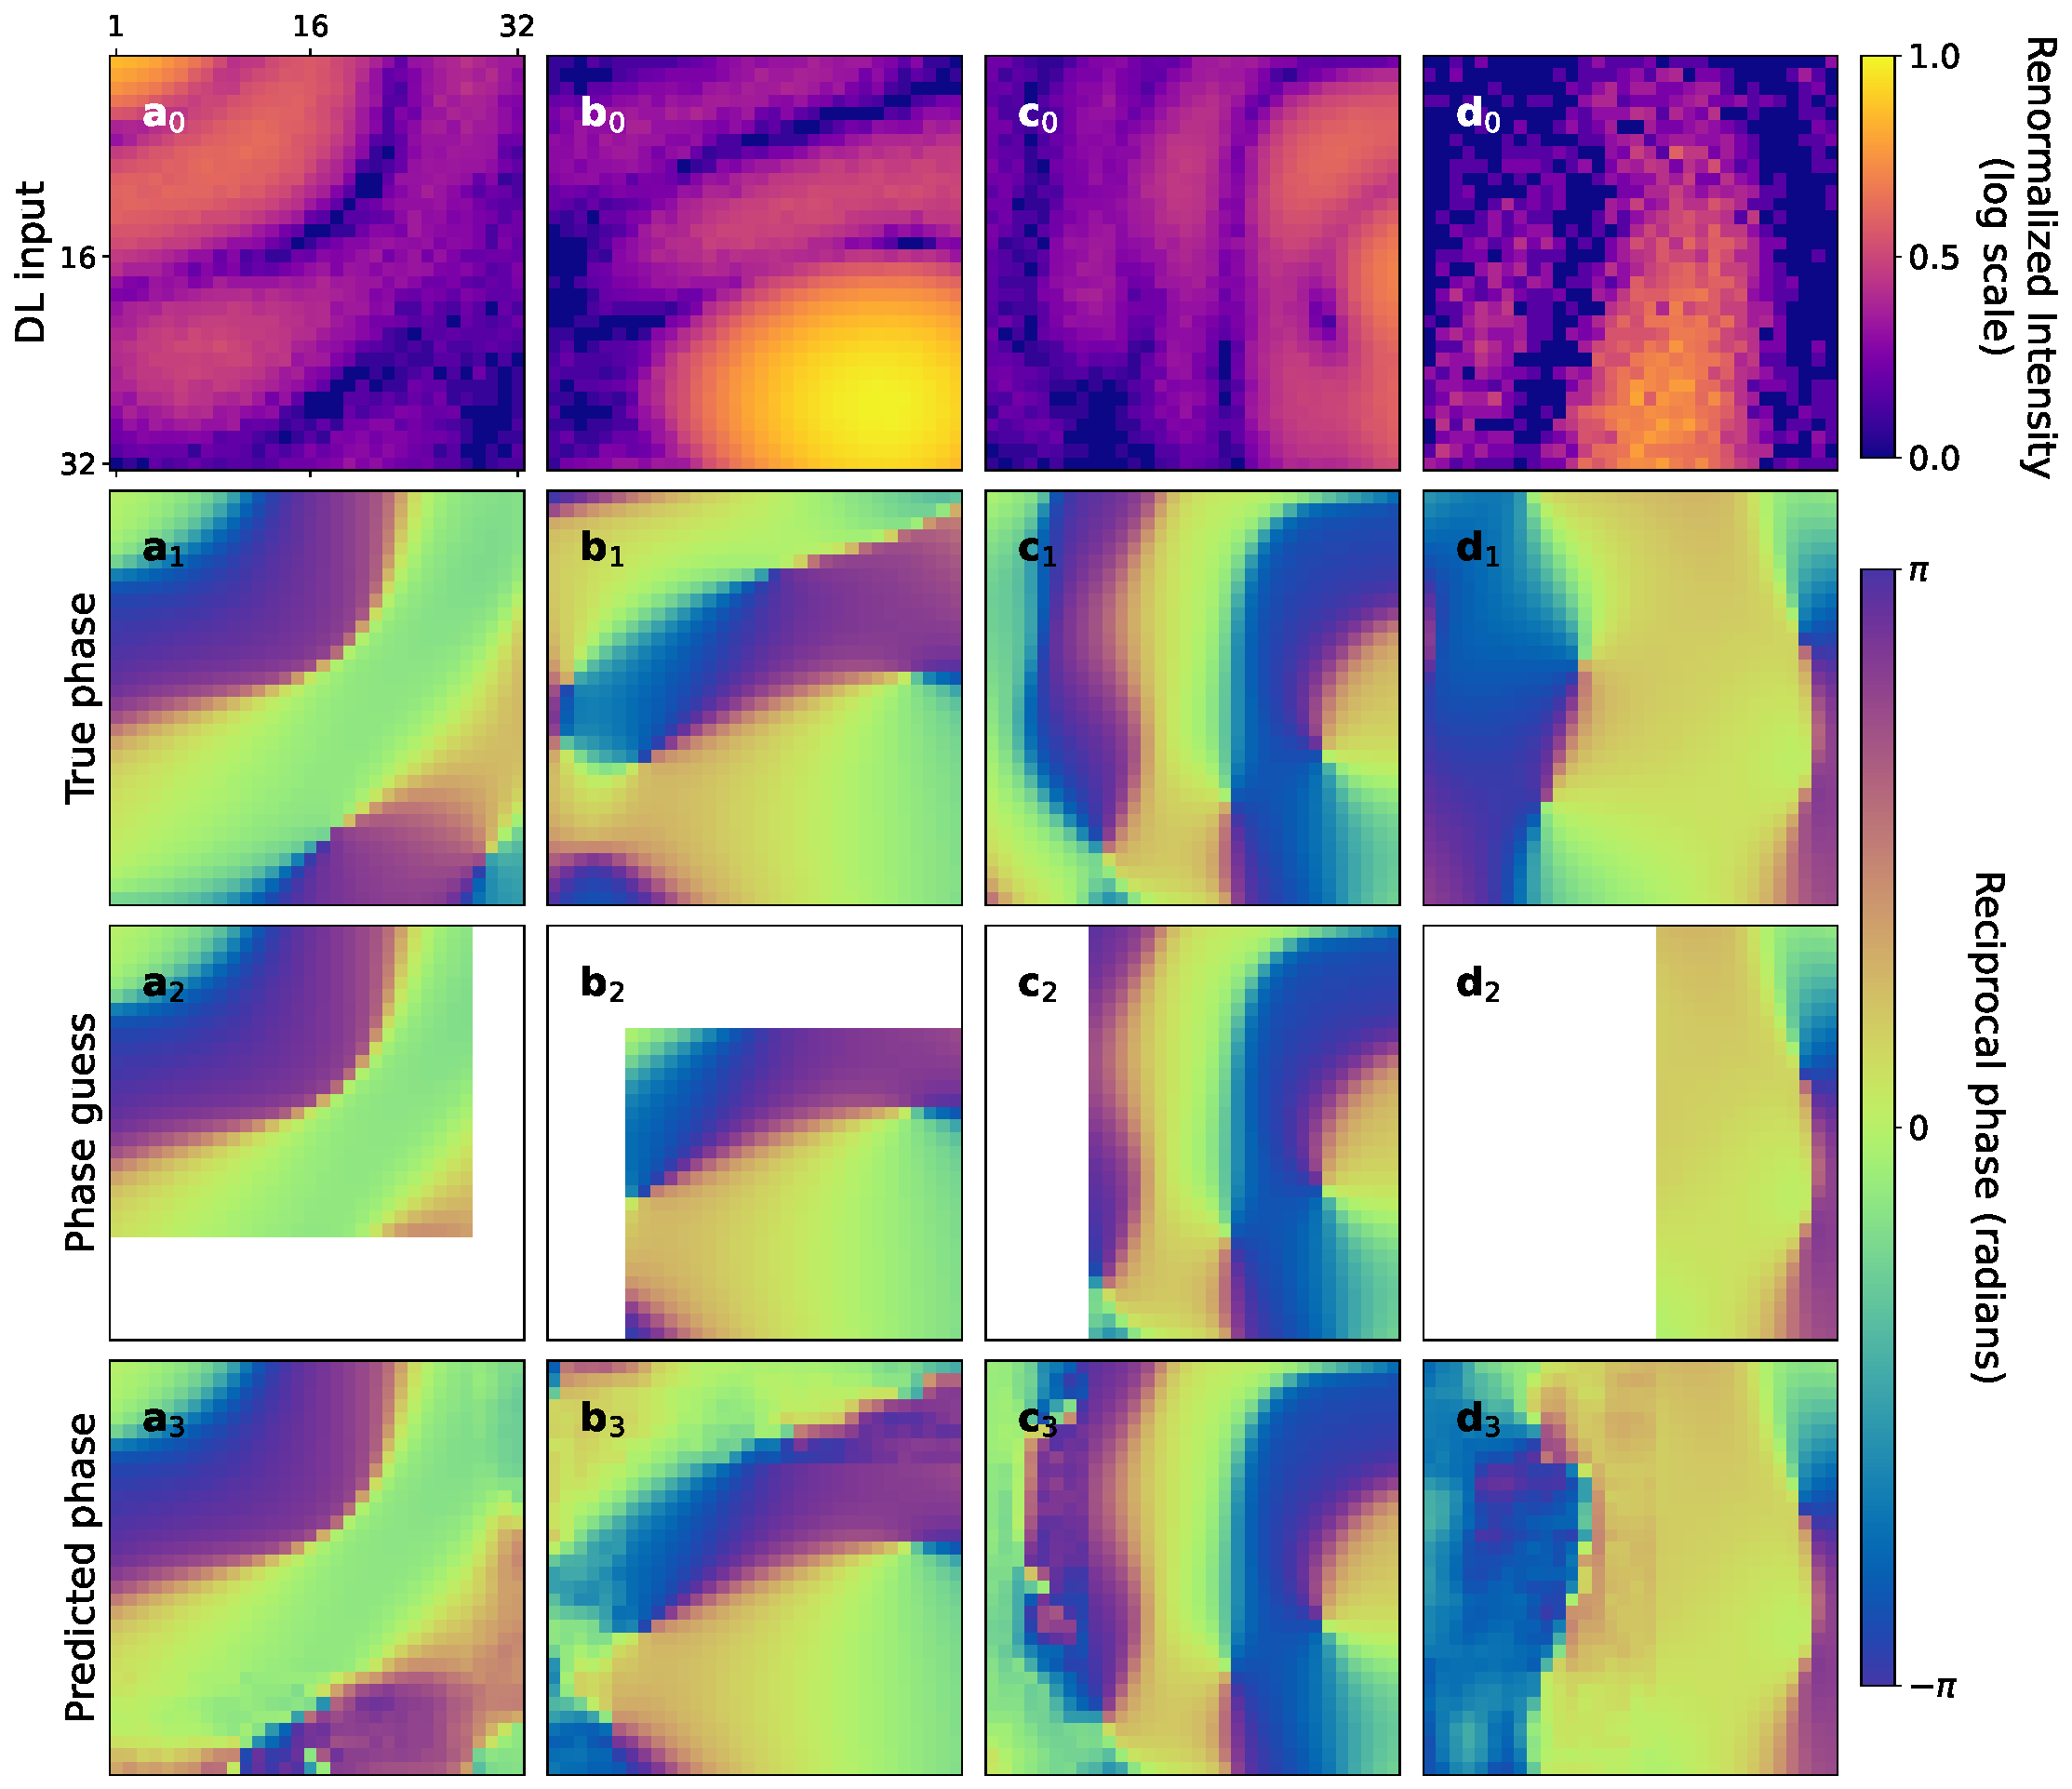
\includegraphics[width=\textwidth]{figures/Phasing/outer_patches_low_strain_RSP.pdf}
    \caption{Examples of RSP prediction for outer patches. The first row shows the central slice of some patches extracted 
    far from the central part of the BCDI peak. The second row shows the ground truth RSP, the third row the RSP initial guess 
    obtained from the overlap with the nearest neighbor of the innermost shell, and the last row shows the 
    DL output. The DL prediction is limited to the missing region. }

    \label{fig:outerpatch_obj_lowstrain}
\end{figure}

\subsection{Results on the full RSP}

Here the results of the combination of the two CNNs are presented for the low-strain case. Once completed the training 
the model was tested on full simulated and experimental BCDI pattern. In order to properly retrieve the full RSP corresponding 
to the diffracted intensity a stitching algorithm for the predicted patches was designed. The stitching takes place
progressively starting from the central patch and updating the full RSP array shell by shell. Once the prediction of the 
central patch RSP is obtained from the first CNN, the patches of intensity belonging to the first shell at distance 10 pixels 
are extracted and the overlapping regions between each patch with the central one are calculated. The predicted central patch RSP 
for each overlapping region is therefore located in the initial guess RSP array that is given to the model as input paired with 
the intensity patch. Subsequently, the full batch of pairs $(I,\varphi_{guess})_{shell = 1}$ is sent through the second CNN and the o
corresponding RSP output is obtained. 
At this stage two main issues have to be considered, namely: (i) during the training of the 
second CNN the initial guess RSP was taken from simulated \textit{ground truth} RSPs while here it is taken from the model's 
previous prediction itself. It is for this reason that any small unavoidable discrepancies between the predicted and 
ground truth RSP can lead the model to further errors. (ii) When a round of RSP is predicted there are overlapping 
regions between patches of the same shell and patches of the previous batch. The most straightforward way to perform the 
stitching of the patches into the full RSP is to overwrite each time the results. However, although a better approach based on 
the average of the overlapping prediction was implemented, the issue did not seem to be fully resolved.
A first test was conducted with this simpler solutions for both issues, and a more robust approach is briefly discussed 
at the end of the section. \\

The crop-predict-stitch method is hence repeated until the last shell. The number of shells and predictions scales with 
the size of the dataset, and it is however always restricted to a spherical region around the Bragg peak. It is therefore 
less accurate for non-cubic data. 
Here, Fig.\ref{fig:stitching_sim_low} shows an example of full RSP stitching for a cubic 128 pixel-sided simulated BCDI 
pattern, while Fig.\ref{fig:stitching_exp_low} reports the analogous result for an experimental data phased with PyNX. 

\begin{figure}[H]
    \centering
    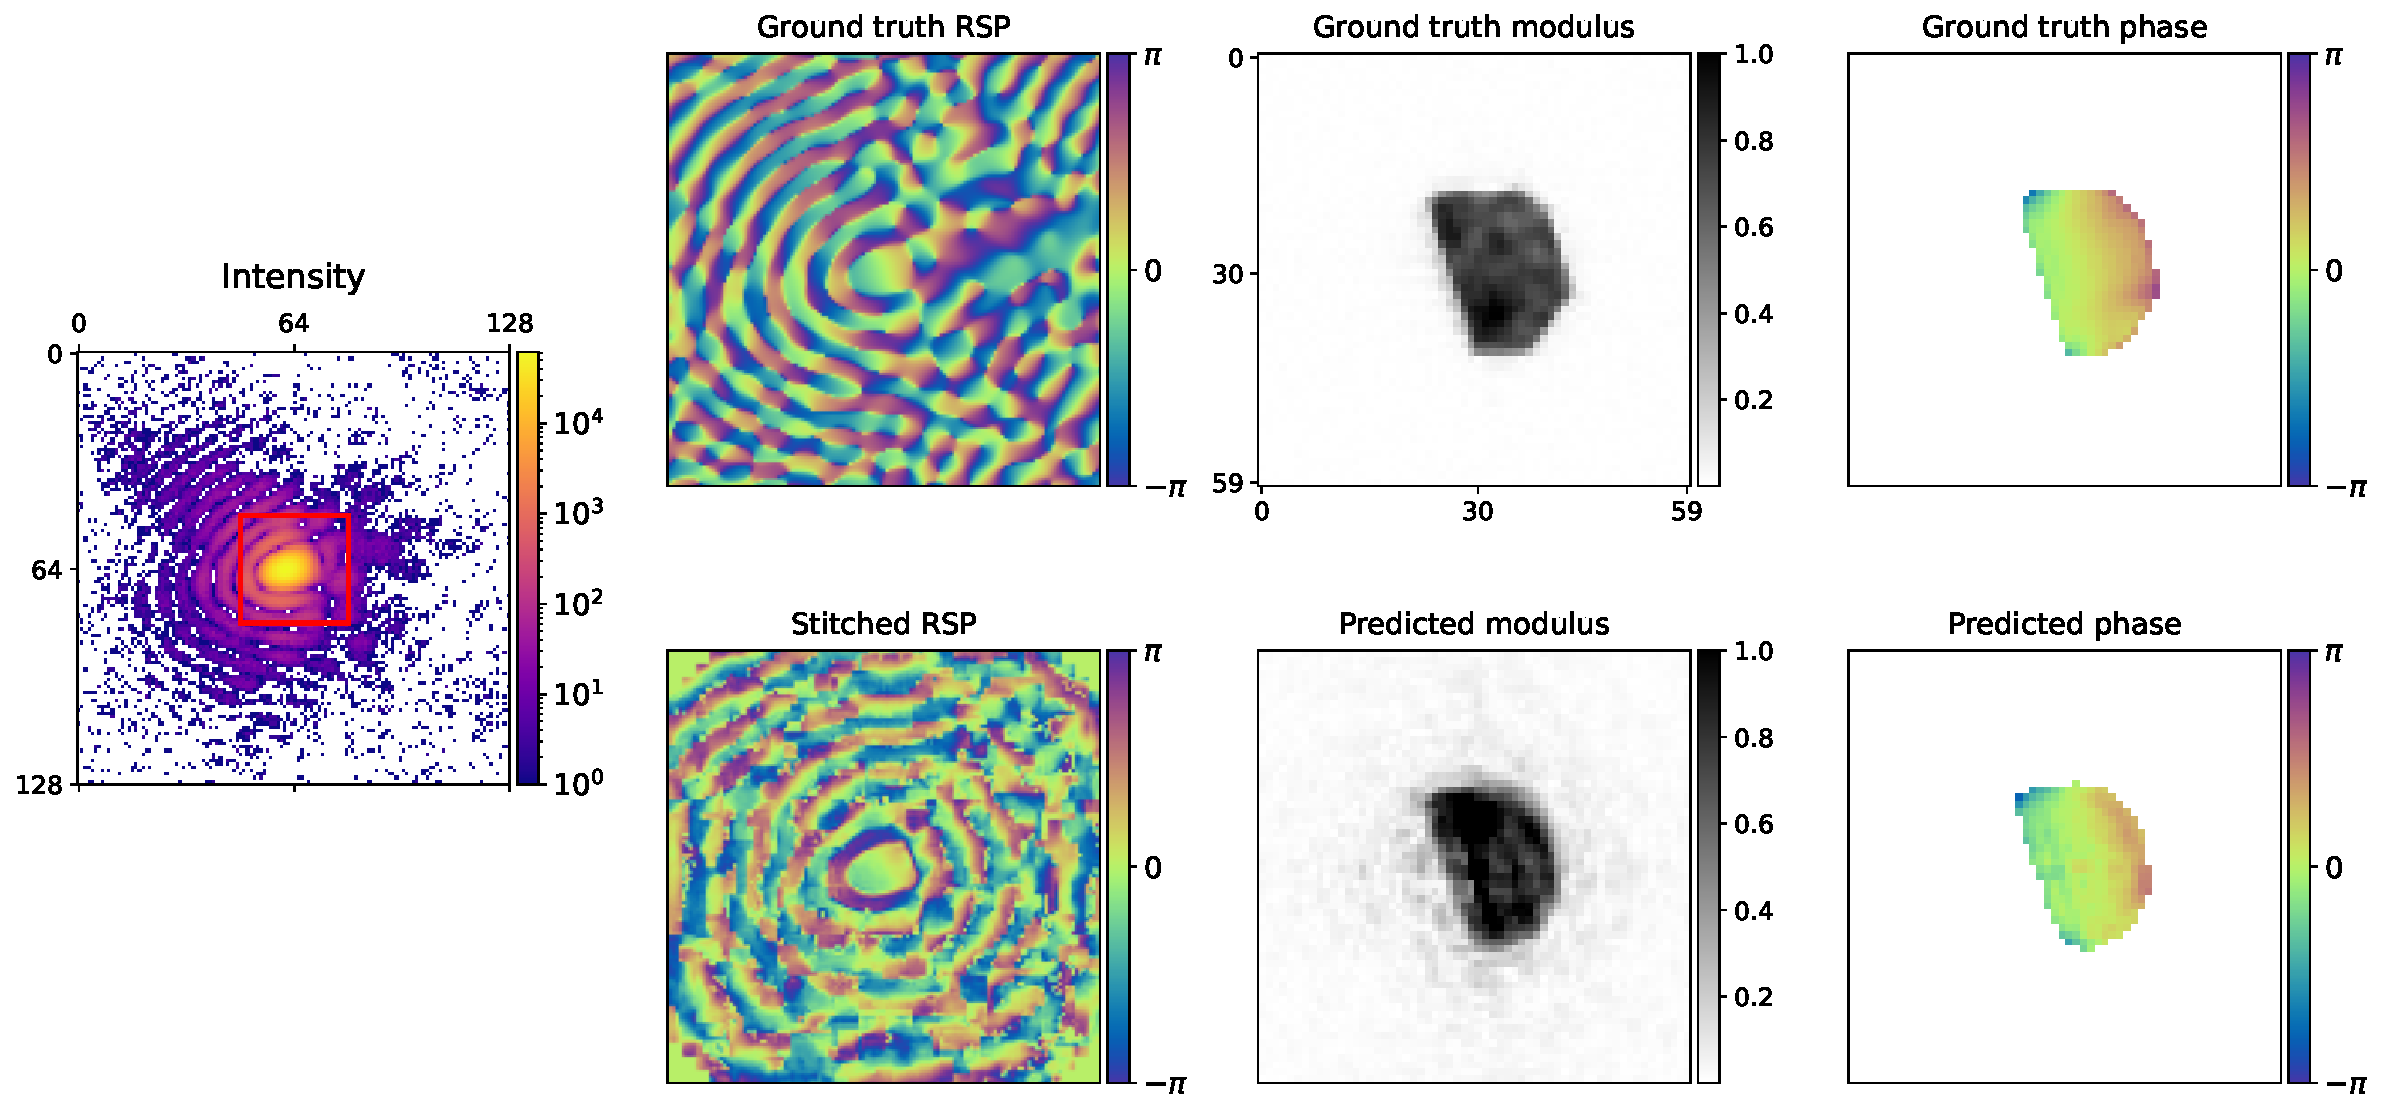
\includegraphics[width=\textwidth]{figures/Phasing/stitching_low_strain_sim.pdf}
    \caption{Results of the stitching of RSP predicted patches for 3D simulated data (central slice displayed). The red 
    square on the intensity figure represents the central patch.}
    \label{fig:stitching_sim_low}
\end{figure}

\begin{figure}[H]
    \centering
    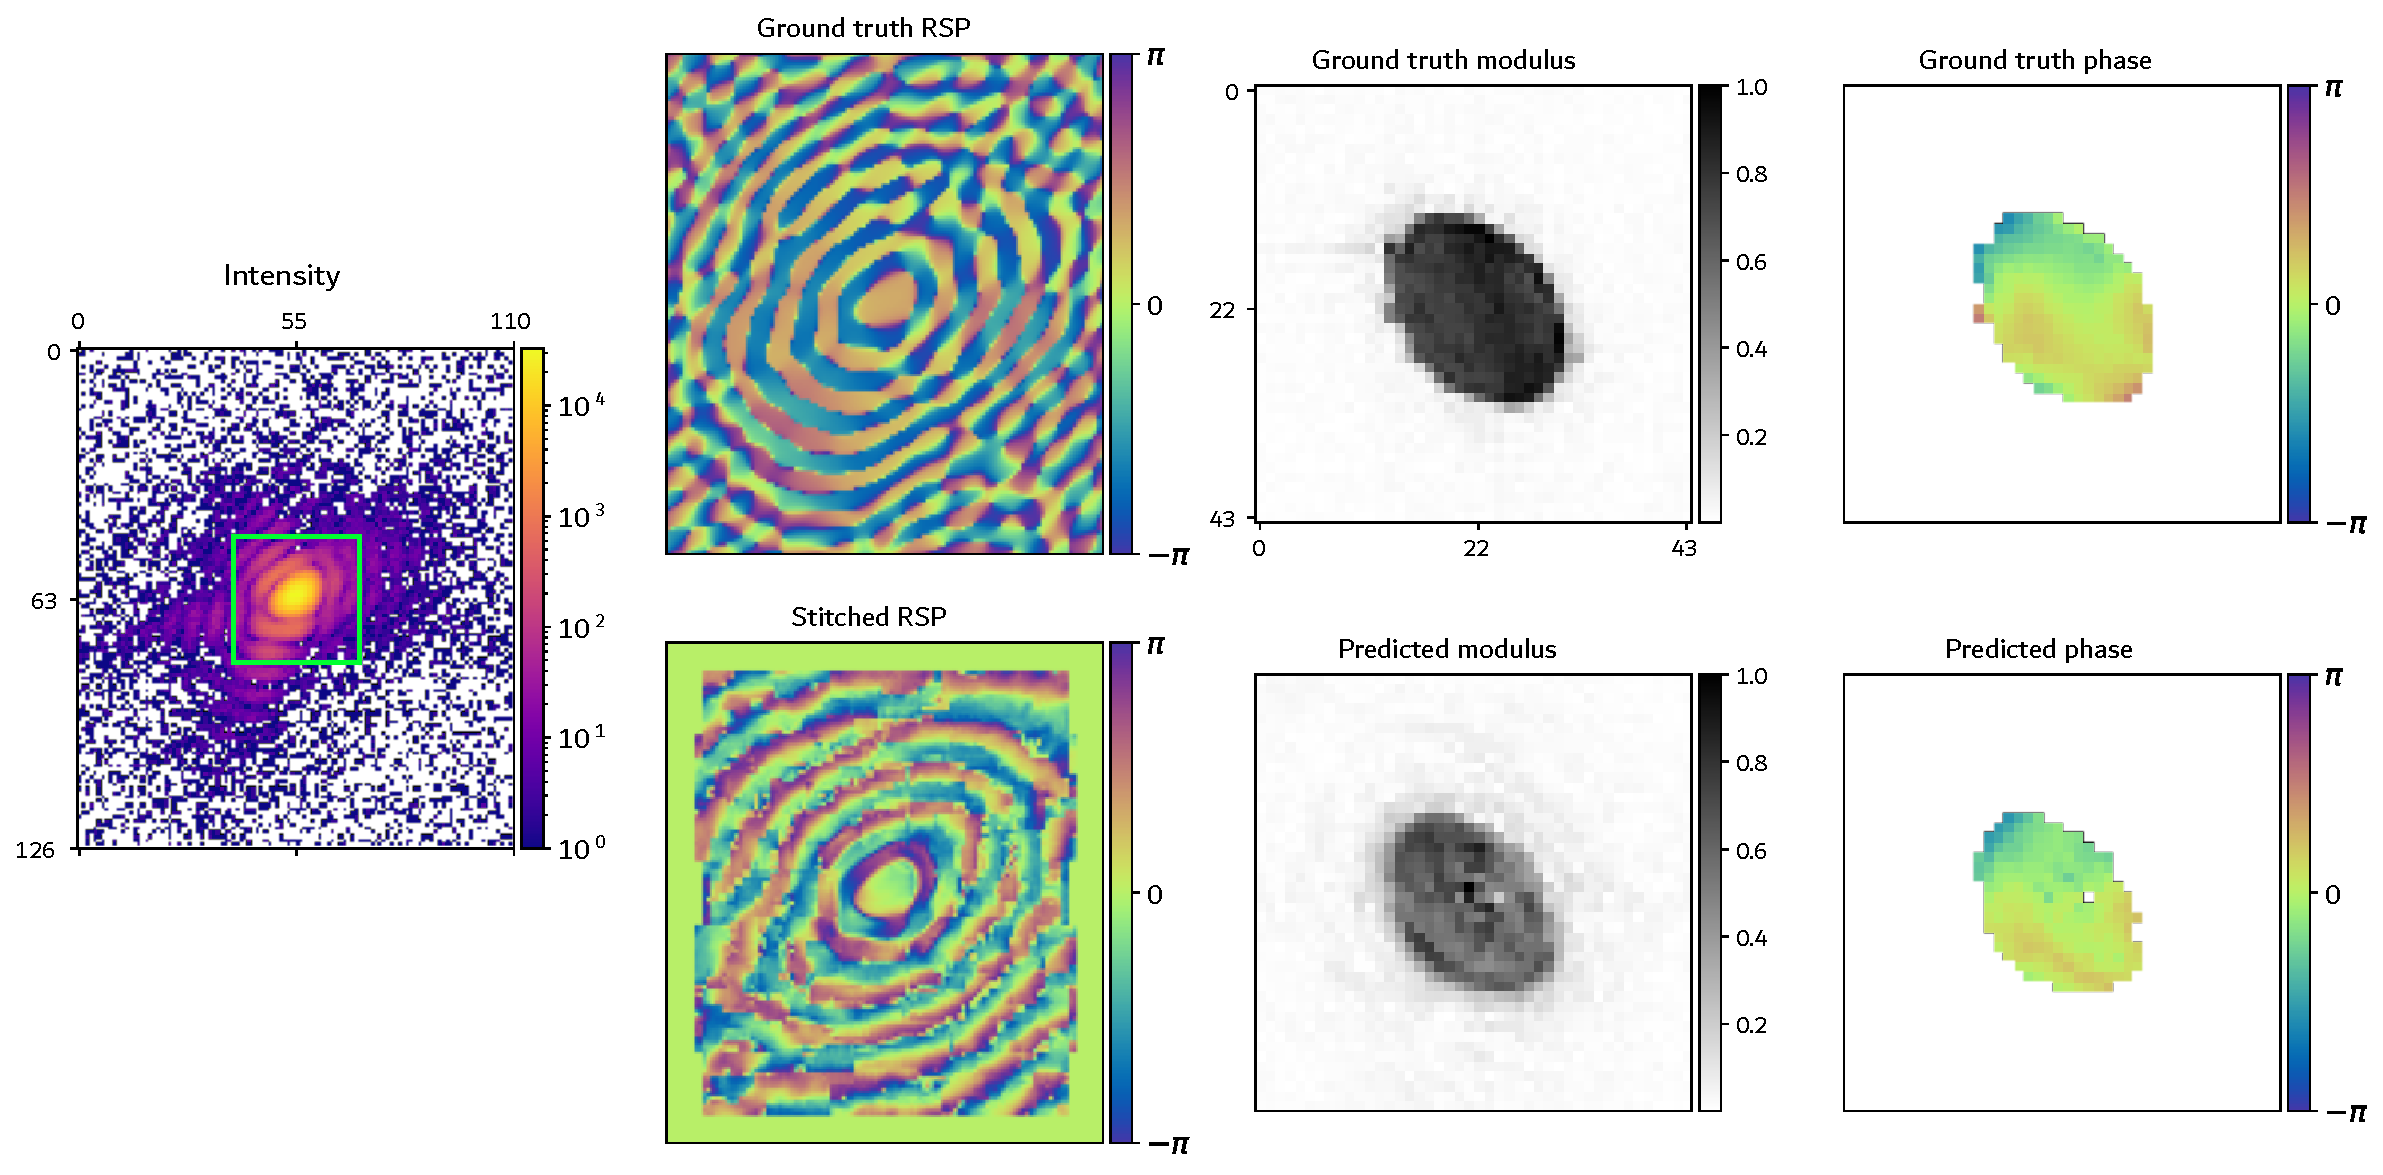
\includegraphics[width=\textwidth]{figures/Phasing/stitching_low_strain_exp.pdf}
    \caption{Results of the stitching of RSP predicted patches for 3D experimental data (central slice displayed).}
    \label{fig:stitching_exp_low}
\end{figure}

What emerges from the above results can be summarized as follows: \\
(i) the accurate prediction of the central RSP patch is fundamental for retrieving the low resolution estimate of the object \\
(ii) the stitching is problematic already from the first shell, most likely because of the two issues pointed out above (
    initial guess from model prediction and RSP averaging of overlapping regions)\\
(iii) the outer RSP patches correctly infer the oversampling ratio as the ``thickness'' of the RSP oscillations matches 
the one of the diffracted intensity, nonetheless, the overall orientation seems to prefer a circular.. \\
(iv) from the reconstructed object's modulus a non-physical more intense spot in the center of the array had to be
filtered out. The occurrence of this spike indicates the presence of wrong zero frequency components in reciprocal
space, hence wrong zero RSP values. Fig. \ref{fig:stitching_filtering} shows the object's modulus before the removal of 
the high intensity spike located in the center. 

\begin{figure}[H]
    \centering
    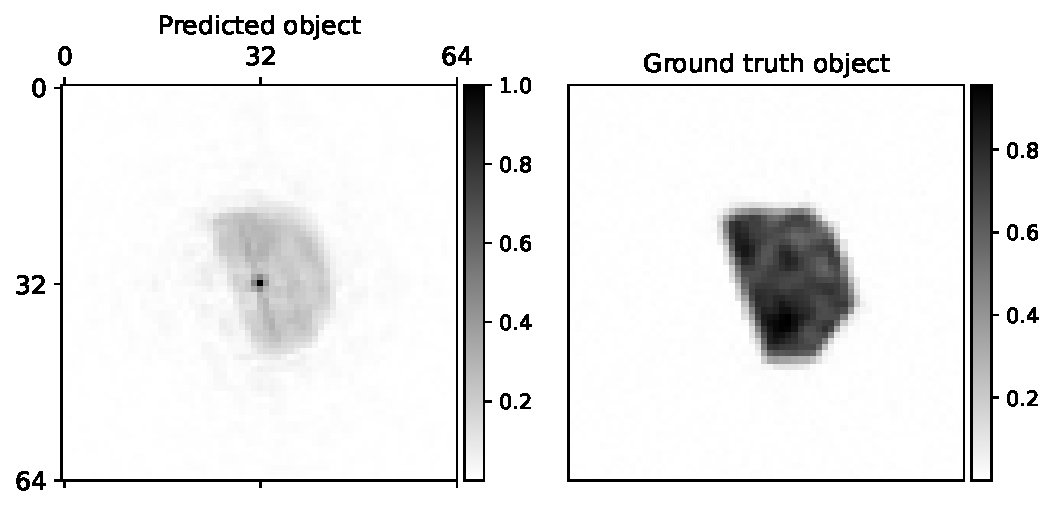
\includegraphics[width=\textwidth]{figures/Phasing/stitching_filtering.pdf}
    \caption{Predicted object's modulus before the filtering of the zero-frequency component.}
    \label{fig:stitching_filtering}
\end{figure}


\section{Patches: 3D case high strain}\label{chp:patches_strain}

For completeness the same model has been trained on a dataset containing highly strained simulated diffraction patterns. 
Each BCDI pattern has been simulated following the procedure explained above in Sec. \ref{sec:dataset_creation3D} and
 \ref{sbsec:patches_creation} for a total amount of 50'000 for both central and outer patches. The two CNN have been trained 
 for 50 epochs each and then tested on new simulated data. 

 For what concerns the firs CNN trained on central patches it was possible to deduce a more difficult learning from the 
 loss curves. While in Fig.\ref{fig:loss_3D_lowstrain} the validation loss reaches 0.3 at the end of the training, for 
Fig.\ref{fig:loss_central_highstrain} it only drops to 0.6 with a significant divergence between training and validation 
starting from the 20th epoch. A higher loss value is nevertheless expected because of the more complex intensity-RSP mapping 
for the high strain cases. 

\begin{figure}[H]
    \centering
    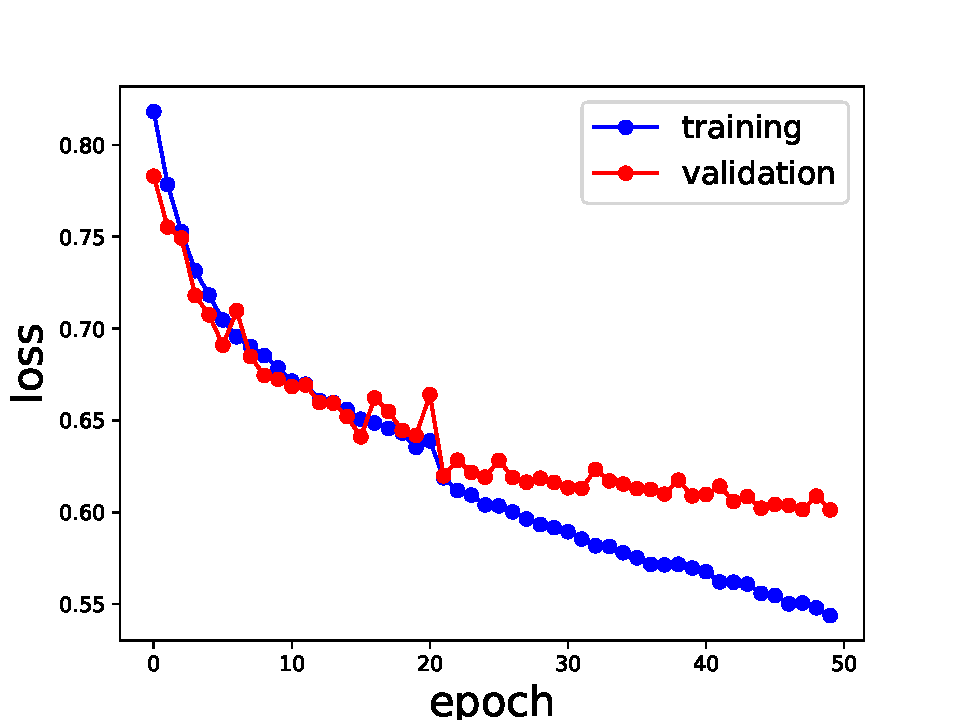
\includegraphics[width=\textwidth]{figures/Phasing/loss_central_patch_highstrain.pdf}
    \caption{Training and validation loss trends for the training of the first CNN on central patches of highly strained BCDI 
    patterns. }
    \label{fig:loss_central_highstrain}
\end{figure}

The results on test data show in fact that the model not always manages to correctly predict the RSP, especially when the 
iso-phase regions are not spherically symmetrical (Fig. \ref{fig:central_highstrain_RSP}c). It however succeeds to 
retrieve the correct RSP oscillations (Fig. \ref{fig:central_highstrain_RSP}a) inside the central fringes elongated by the
high strain. The reconstructions in real space, shown in Fig. \ref{fig:central_highstrain_obj}, confirm satisfactory 
result for the first column and poor for the third column. 

\begin{figure}[H]
    \centering
    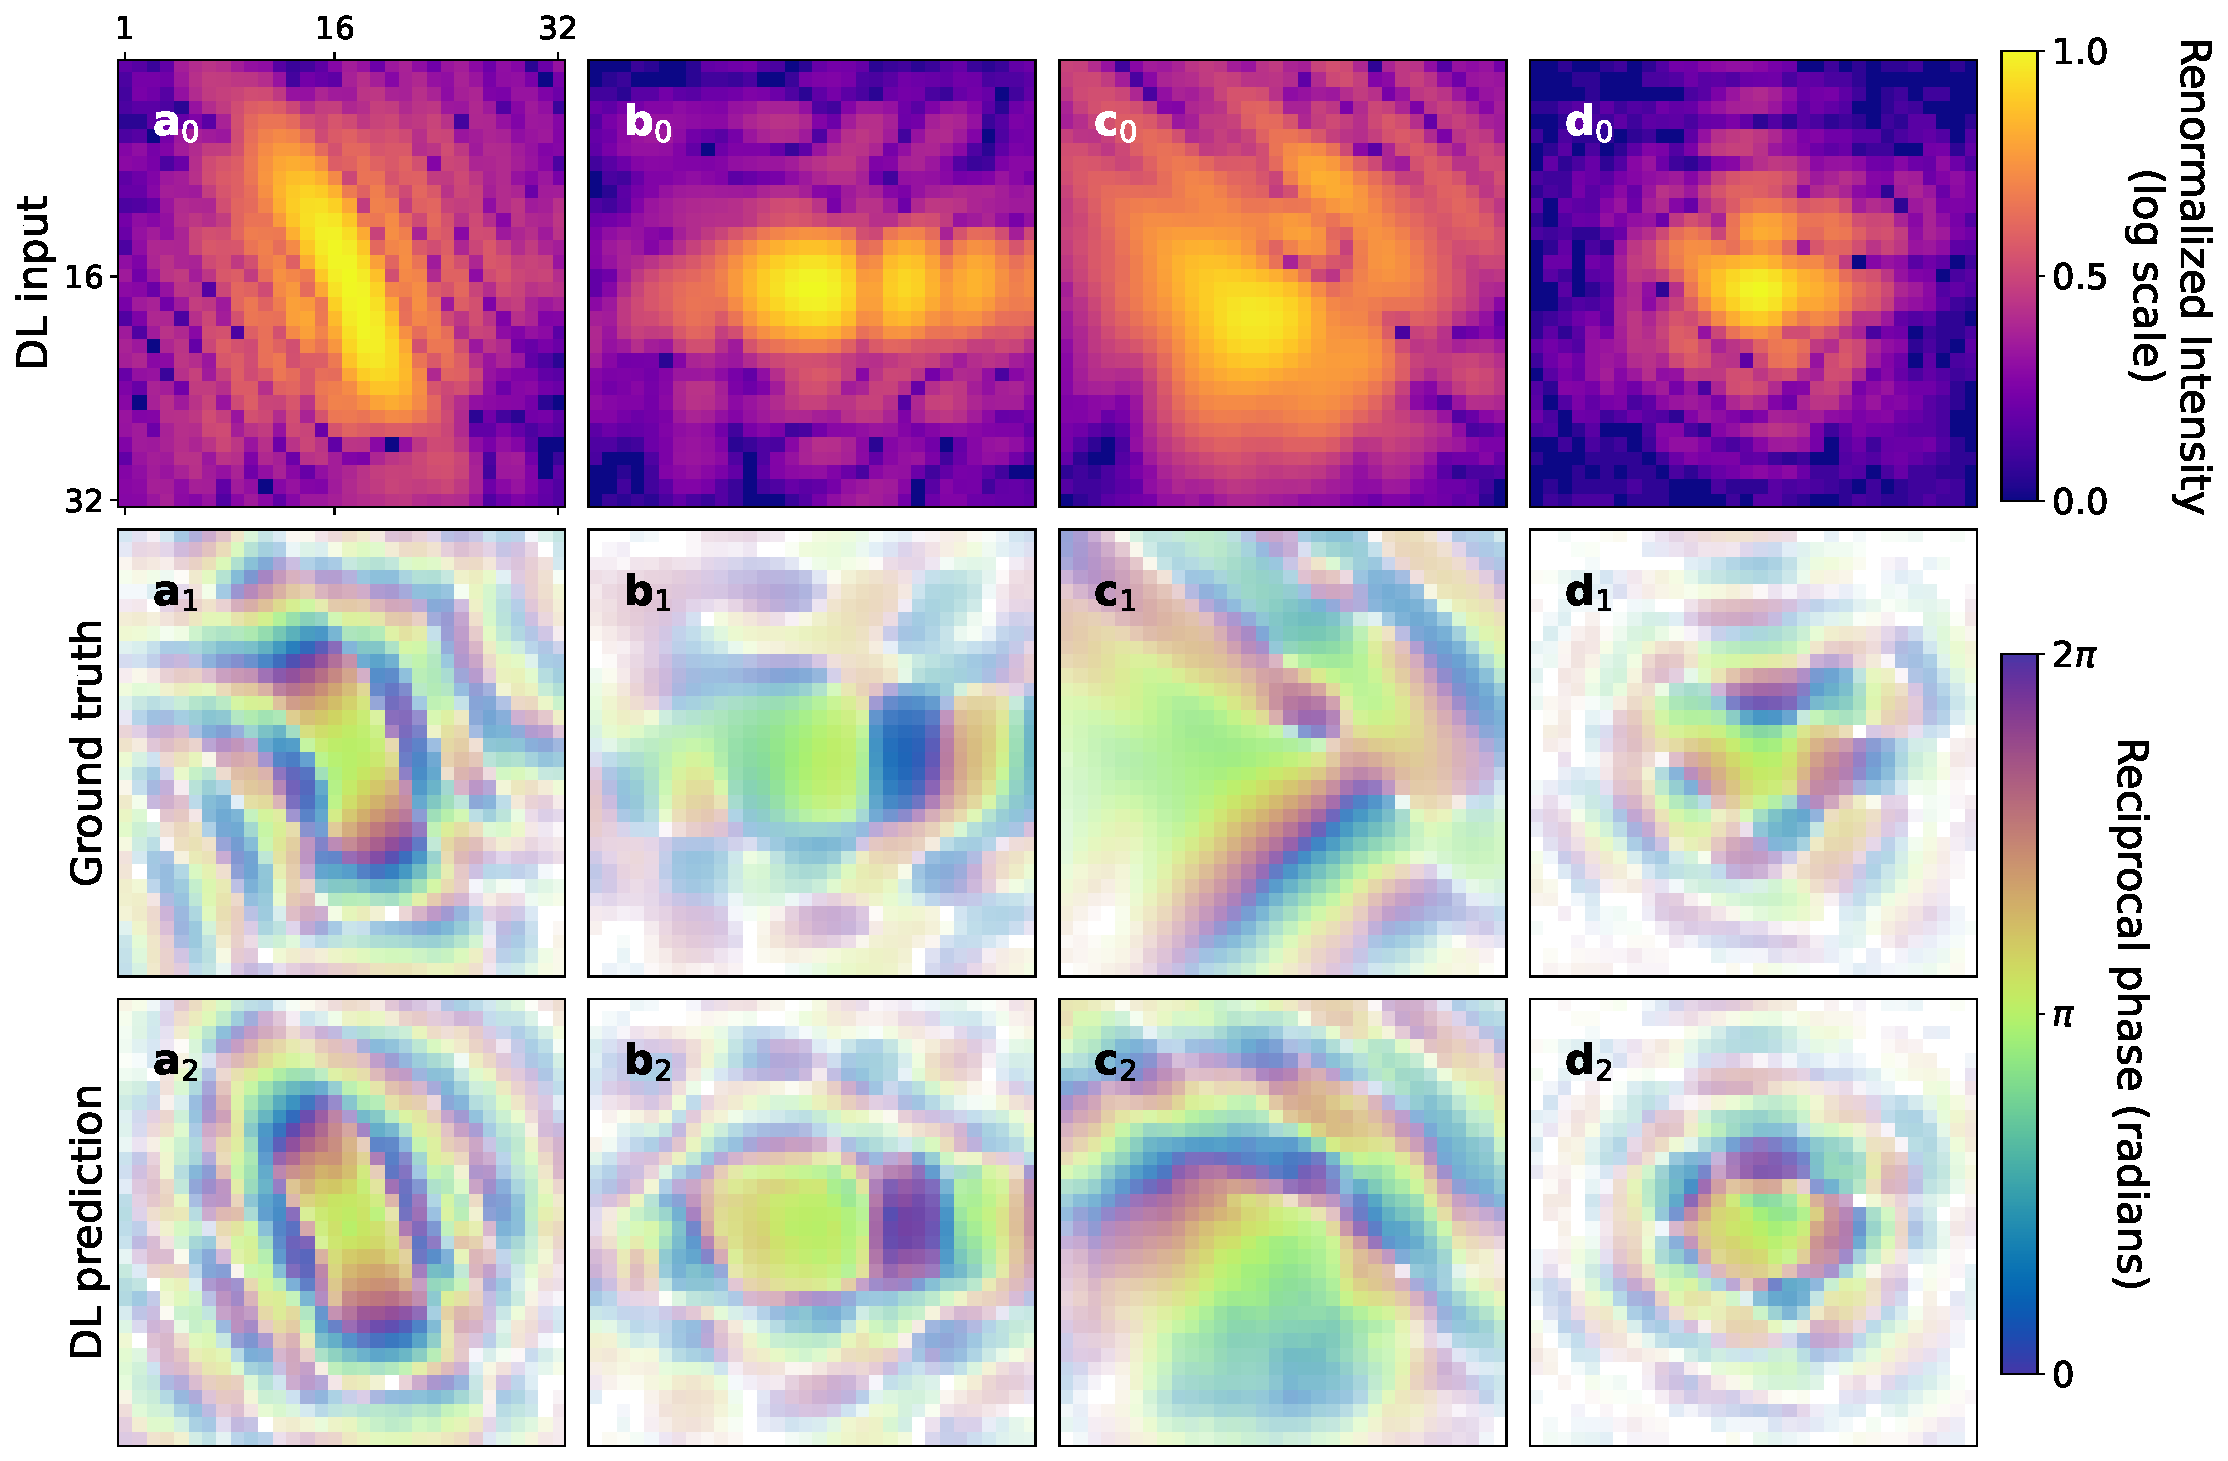
\includegraphics[width=\textwidth]{figures/Phasing/central_patch_highstrain_RSP.pdf}
    \caption{}
    \label{fig:central_highstrain_RSP}
\end{figure}

\begin{figure}[H]
    \centering
    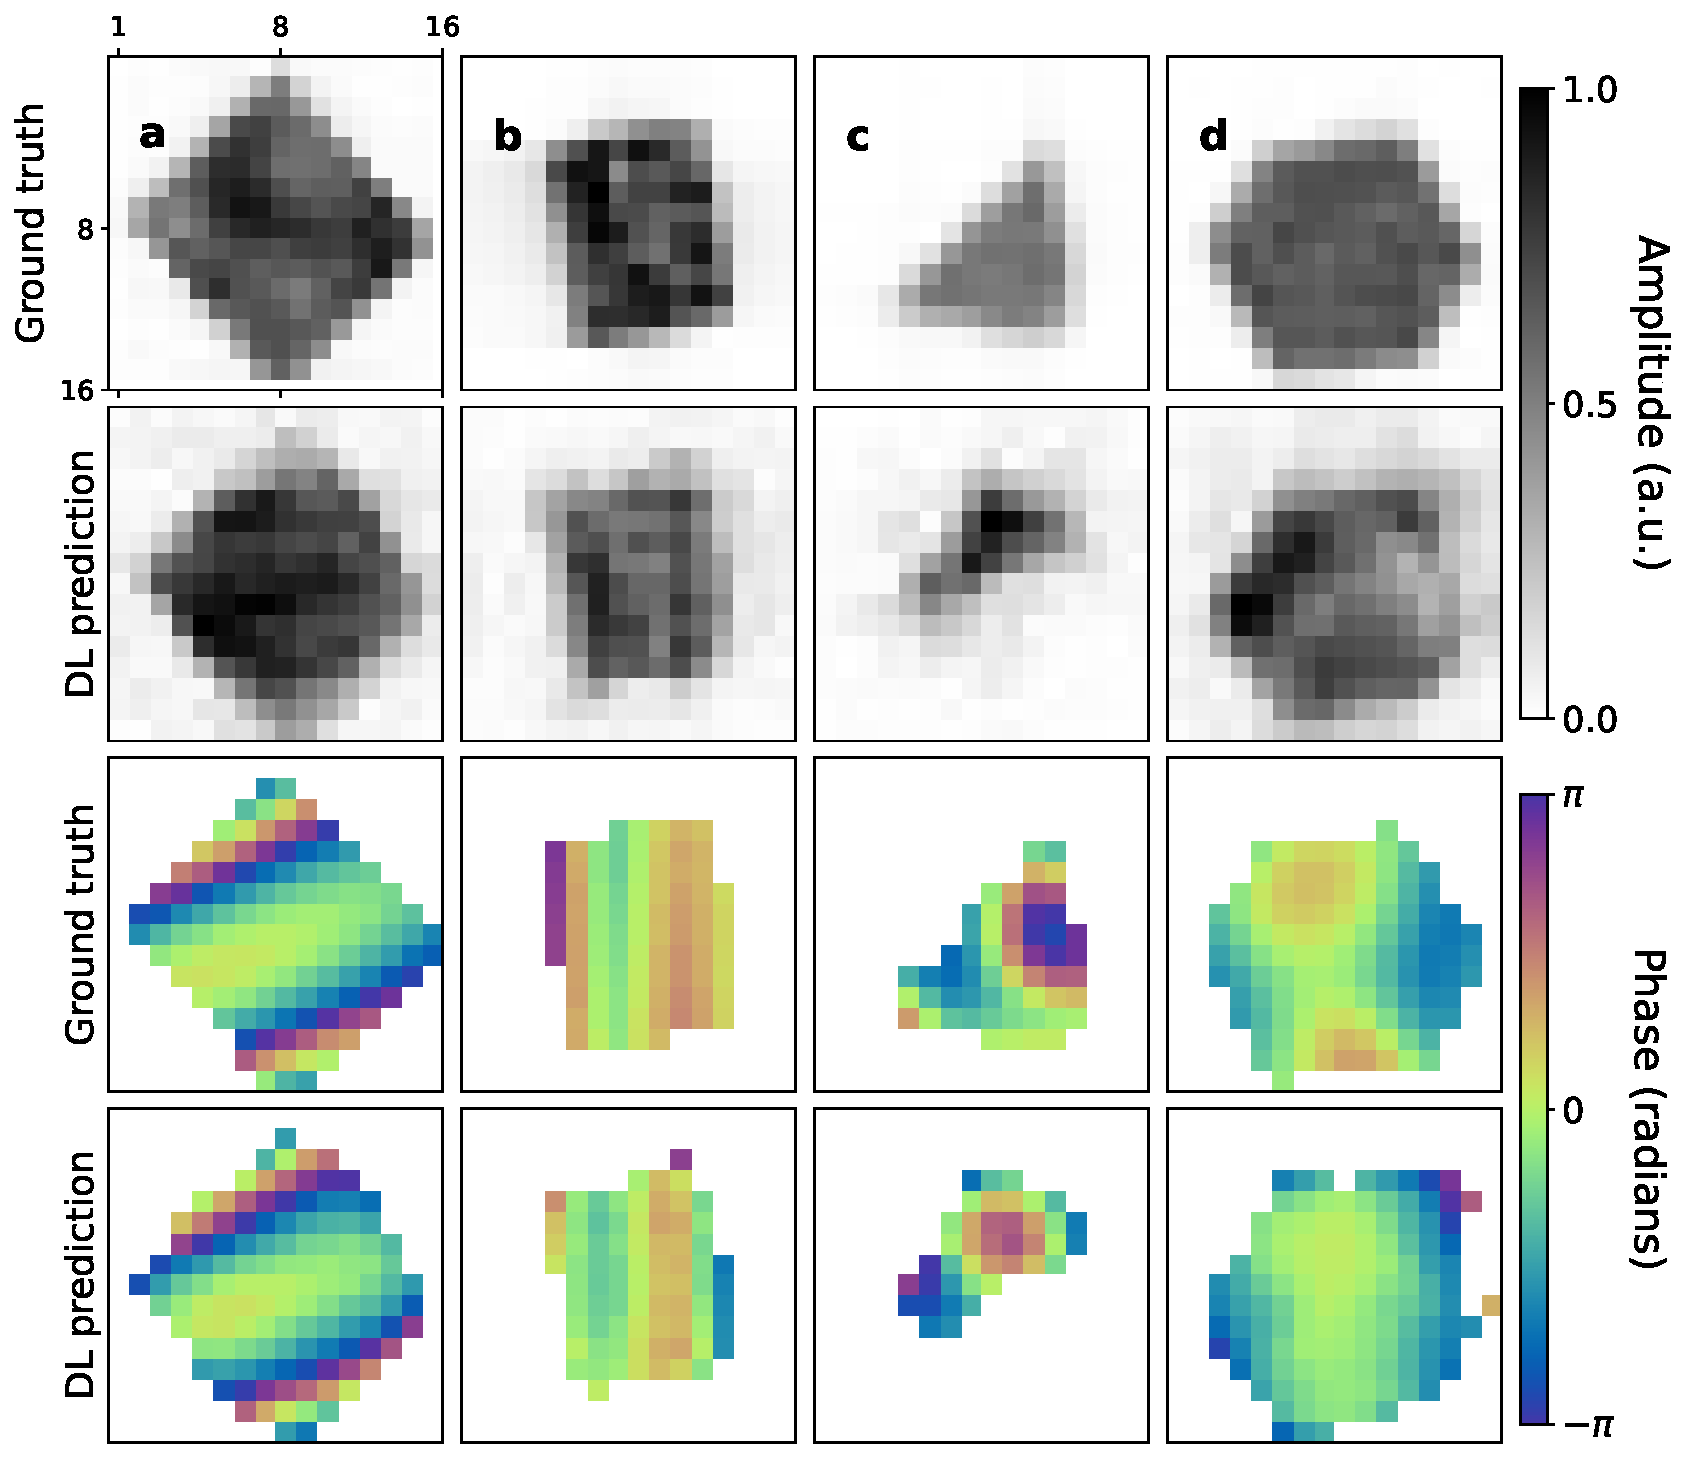
\includegraphics[width=\textwidth]{figures/Phasing/central_patch_highstrain_obj.pdf}
    \caption{}
    \label{fig:central_highstrain_obj}
\end{figure}

Regarding the second CNN trained on patches instead, one can observe that the performance is not severely affected by the 
high-strain. Strong discrepancies between predicted and ground truth RSP are mostly present where there is no intensity signal, 
thus not relevant (see Fig.\ref{fig:outer_highstrain}). The good accuracy of on the outer patches predictions suggests that the crucial and more challenging 
mapping to retrieve involves the central patch mostly. 
\begin{figure}[H]
    \centering
    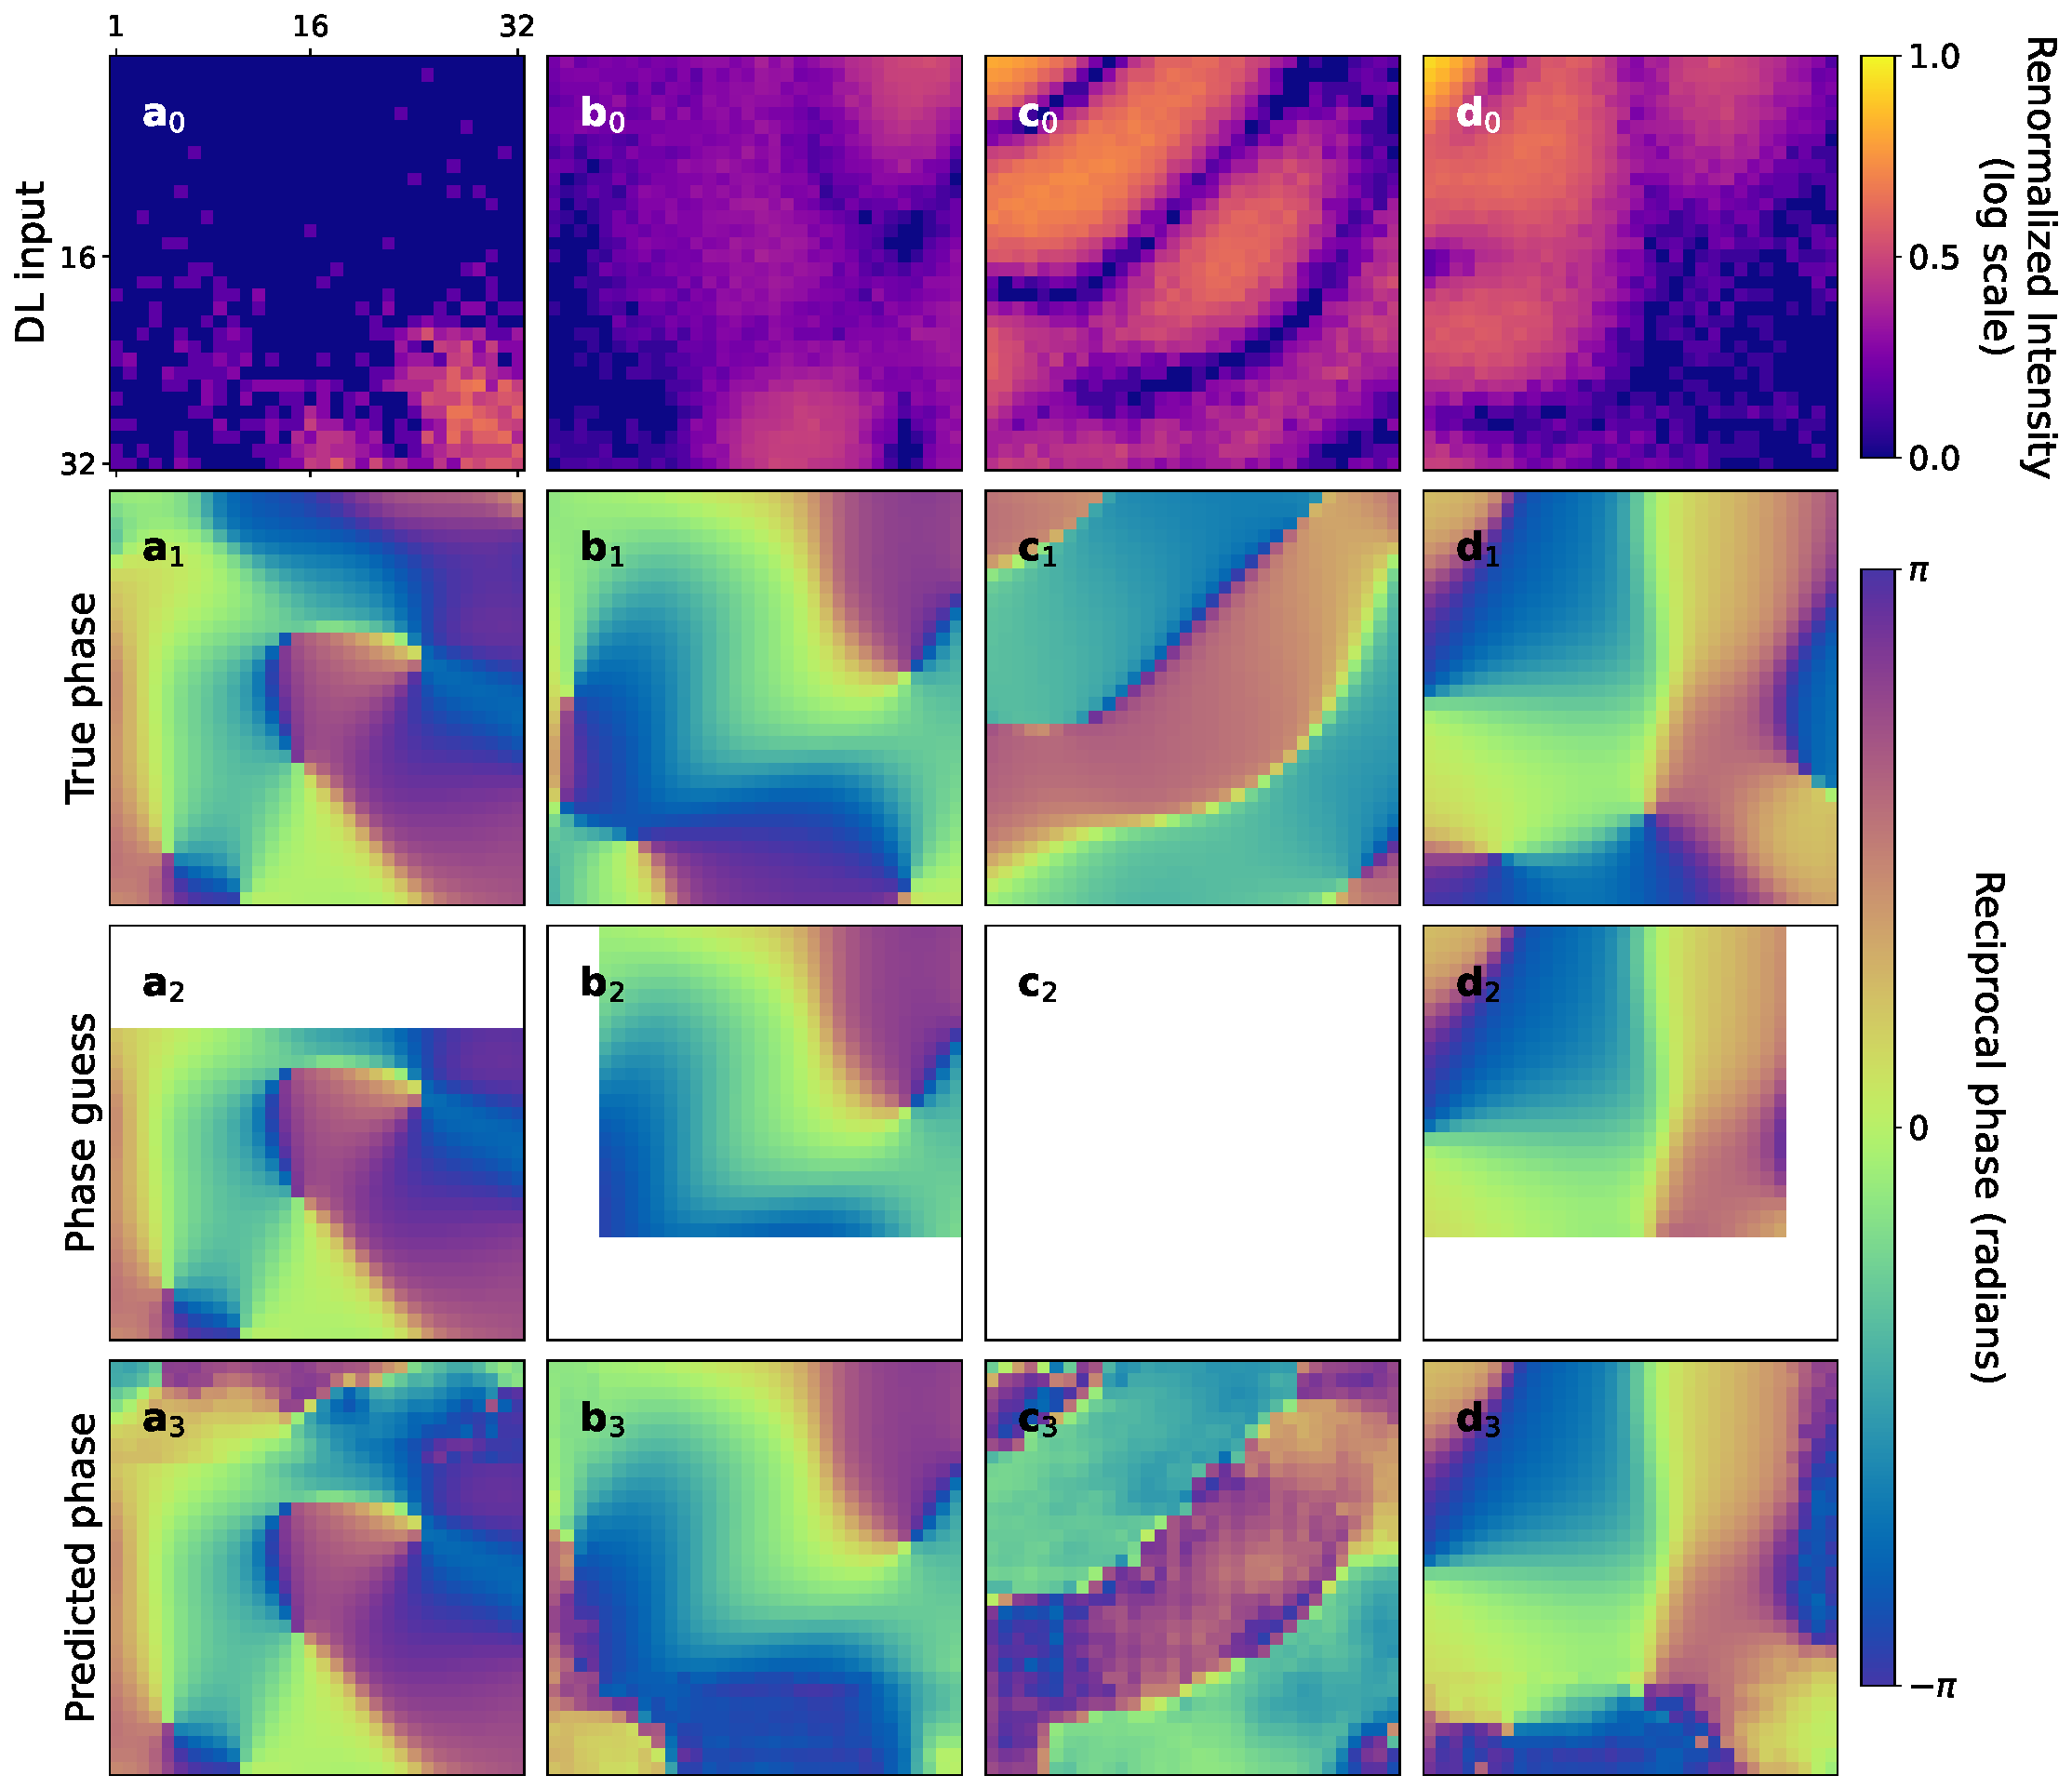
\includegraphics[width=\textwidth]{figures/Phasing/outer_patches_high_strain_RSP.pdf}
    \caption{}
    \label{fig:outer_highstrain}
\end{figure}
For completeness, it is shown here (Fig.\ref{fig:stitching_highstrain}) the result of the full RSP stitching and the corresponding reconstructed object for 
the high-strain case as well. A simulated test data has been used for the ground truth comparison. It is clear that the 
stitching algorithm is performing poorly as observed for the low-strain case. However, the central RSP patch is fairly 
similar to the ground truth and therefore the low resolution reconstructed object shows roughly the correct shape and 
phase. 

\begin{figure}[H]
    \centering
    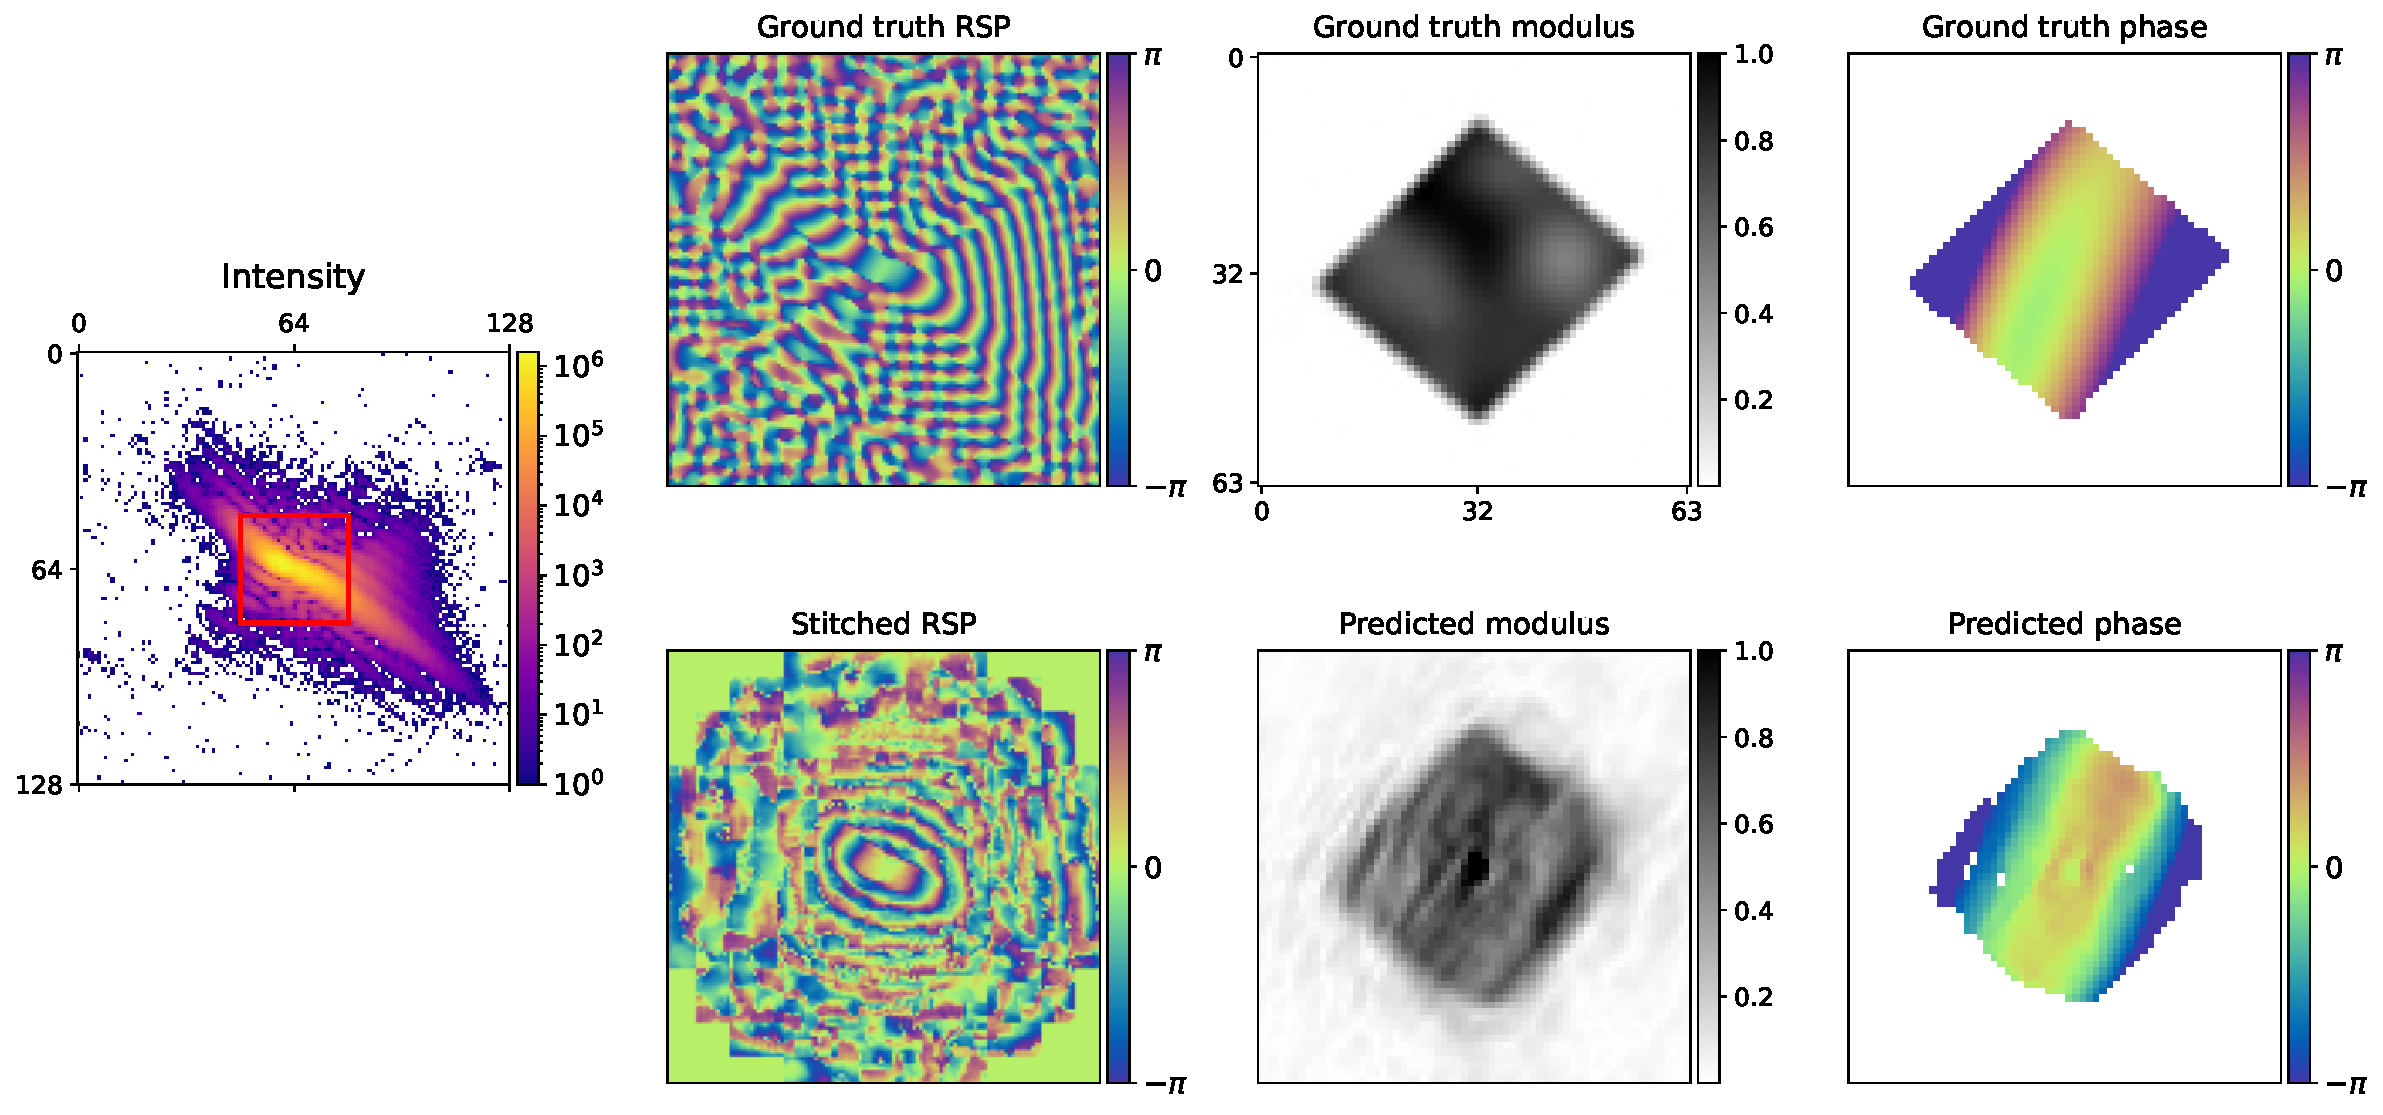
\includegraphics[width=\textwidth]{figures/Phasing/stitching_high_strain_sim.pdf}
    \caption{}
    \label{fig:stitching_highstrain}
\end{figure}

\subsection{Discussion}
Although failed, this study on the prediction of the RSP in smaller patches has led to better understanding of the problem 
and nevertheless unveiled some interesting insights. For instance, it showed that the retrieval of the mapping between patches 
is possible with a CNN trained with the WCA loss function, untying even more the relationship with the real space object. 
Moreover, it emerged that the main difficulty of this approach is given by the stitching of the RSP patches into the full 
array. As mentioned above, the hypothesized reasons for this problem are (i) the fact that the model ``sees'' 
simulated ground truth RSP guesses during the training and predicted ones during inference, and (ii) the averaging 
of RSP predictions for overlapping voxels. In order to overcome these limitations other approaches were contemplated but 
never realized for lack of time. In particular, it was imagined a way to extract, analyze and stitch the patches inside the 
model into a sort of Recurrent Convolutional Neural Network (RCNN) that would keep track of the previous innermost shell
thanks to a dedicated convolutional Long-Short Term Memory (LSTM) \cite{shi2015convolutionallstmnetworkmachine}. By doing 
this the model would always be exposed to its own RSP predictions as initial guess for outer patches and the RSP average over
overlapping voxels could be replaced with a convolutional layer with non-linear activation function. While the attempts 
of setting up such model are not reported here, it is mentioned the idea as possible inspiration for future works. \\

To conclude, main finding of this study on patches is that it is crucial for a good object estimate to accurately predict 
the RSP in the vicinity of the center of the Bragg peak, and that the CNN model trained with the WCA can accomplish this task 
for highly strained patterns as well. It was therefore decided to invest the efforts into a regular CNN for the prediction 
of the RSP of 3D highly strained BCDI patterns with the intermediate size of $64\times64\times64$ pixels. 


% MODEL 3D CASE STRAIN WITH PATCHES: SHOW THE FAILURE AND EXPLAIN WHY 

\section{Model design: 3D case high strain }\label{chp:3d_nostrain}
% MODEL 3D CASE STRAIN FULL DIFFRACTION 

\section{Results on 3D case}\label{chp:phasing}
\section{Refinement with iterative algorithms}\label{chp:phasing}
\section{Experimental results}\label{chp:phasing}

